% This is the Reed College LaTeX thesis template. Most of the work
% for the document class was done by Sam Noble (SN), as well as this
% template. Later comments etc. by Ben Salzberg (BTS). Additional
% restructuring and APA support by Jess Youngberg (JY).
% Your comments and suggestions are more than welcome; please email
% them to cus@reed.edu
%
% See https://www.reed.edu/cis/help/LaTeX/index.html for help. There are a
% great bunch of help pages there, with notes on
% getting started, bibtex, etc. Go there and read it if you're not
% already familiar with LaTeX.
%
% Any line that starts with a percent symbol is a comment.
% They won't show up in the document, and are useful for notes
% to yourself and explaining commands.
% Commenting also removes a line from the document;
% very handy for troubleshooting problems. -BTS

% As far as I know, this follows the requirements laid out in
% the 2002-2003 Senior Handbook. Ask a librarian to check the
% document before binding. -SN

%%
  %% Preamble
%%
  % \documentclass{<something>} must begin each LaTeX document
\documentclass[12pt,twoside]{smiththesis}
% Packages are extensions to the basic LaTeX functions. Whatever you
% want to typeset, there is probably a package out there for it.
% Chemistry (chemtex), screenplays, you name it.
% Check out CTAN to see: https://www.ctan.org/
  %%
  \usepackage{graphicx,latexsym}
\usepackage{amsmath}
\usepackage{amssymb,amsthm}
\usepackage{longtable,booktabs,setspace}
\usepackage{chemarr} %% Useful for one reaction arrow, useless if you're not a chem major
\usepackage[hyphens]{url}
% Added by CII
\usepackage{hyperref}
\usepackage{lmodern}
\usepackage{multicol}
\usepackage{float}
\floatplacement{figure}{H}
% End of CII addition
\usepackage{rotating}
%\hypersetup{
%    colorlinks=true,
%    linkcolor=blue,
%    filecolor=magenta,      
 %   urlcolor=blue,
 %   pdftitle={Overleaf Example},
 %   pdfpagemode=FullScreen,
 %   }

% Next line commented out by CII
%%% \usepackage{natbib}
% Comment out the natbib line above and uncomment the following two lines to use the new
% biblatex-chicago style, for Chicago A. Also make some changes at the end where the
% bibliography is included.
%\usepackage{biblatex-chicago}
%\bibliography{thesis}


% Added by CII (Thanks, Hadley!)
% Use ref for internal links
\renewcommand{\hyperref}[2][???]{\autoref{#1}}
\def\chapterautorefname{Chapter}
\def\sectionautorefname{Section}
\def\subsectionautorefname{Subsection}
% \hypersetup{
%     colorlinks=true,
%     linkcolor=blue,
%    filecolor=blue,
%     citecolor = blue,      
%     urlcolor=cyan,
 %    }
\hypersetup{colorlinks=true,
            linkcolor=blue,
            citecolor=black,
            urlcolor=blue}
% End of CII addition

% Added by CII
\usepackage{caption}
\captionsetup{width=5in}
% End of CII addition

% \usepackage{times} % other fonts are available like times, bookman, charter, palatino
\usepackage{palatino}
\usepackage{tcolorbox}

% Syntax highlighting #22

% To pass between YAML and LaTeX the dollar signs are added by CII
\title{Estimating Unobserved COVID-19 Infections in the United States}
\author{Quinn White}
% The month and year that you submit your FINAL draft TO THE LIBRARY (May or December)
\date{May 2023}
\division{Mathematics and Natural Sciences}
\advisor{Ben Baumer}
\institution{Smith College}
\degree{Bachelor of Arts}
%If you have two advisors for some reason, you can use the following
% Uncommented out by CII
\altadvisor{Nicholas Reich}
% End of CII addition

%%% Remember to use the correct department!
\department{Statistical and Data Sciences}
% if you're writing a thesis in an interdisciplinary major,
% uncomment the line below and change the text as appropriate.
% check the Senior Handbook if unsure.
%\thedivisionof{The Established Interdisciplinary Committee for}
% if you want the approval page to say "Approved for the Committee",
% uncomment the next line
%\approvedforthe{Committee}

% Added by CII
%%% Copied from knitr
%% maxwidth is the original width if it's less than linewidth
%% otherwise use linewidth (to make sure the graphics do not exceed the margin)
\makeatletter
\def\maxwidth{ %
  \ifdim\Gin@nat@width>\linewidth
    \linewidth
  \else
    \Gin@nat@width
  \fi
}
\makeatother

\newlength{\csllabelwidth}
\setlength{\csllabelwidth}{3em}
\newlength{\cslhangindent}
\setlength{\cslhangindent}{1.5em}
% for Pandoc 2.8 to 2.10.1
\newenvironment{cslreferences}%
  {}%
  {\par}
% For Pandoc 2.11+
% As noted by @mirh [2] is needed instead of [3] for 2.12
\newenvironment{CSLReferences}[2] % #1 hanging-ident, #2 entry spacing
 {% don't indent paragraphs
\setlength{\parindent}{0pt}
% turn on hanging indent if param 1 is 1
\ifodd #1 \everypar{\setlength{\hangindent}{\cslhangindent}}\ignorespaces\fi
% set entry spacing
\ifnum #2 > 0
\setlength{\parskip}{#2\baselineskip}
  \fi
}%
{}
\usepackage{calc} % for calculating minipage widths
\newcommand{\CSLBlock}[1]{#1\hfill\break}
  \newcommand{\CSLLeftMargin}[1]{\parbox[t]{\csllabelwidth}{#1}}
    \newcommand{\CSLRightInline}[1]{\parbox[t]{\linewidth - \csllabelwidth}{#1}}
      \newcommand{\CSLIndent}[1]{\hspace{\cslhangindent}#1}
        \renewcommand{\contentsname}{Table of Contents}
% End of CII addition

\setlength{\parskip}{0pt}

% Added by CII

\providecommand{\tightlist}{%
  \setlength{\itemsep}{0pt}\setlength{\parskip}{0pt}}

\Acknowledgements{
Will add
}

\Dedication{
You can have a dedication here if you wish.
}


\Abstract{
As we have navigated the COVID-19 pandemic, case counts have been a central source of information for understanding transmission dynamics and the effect of public health interventions. However, because the number of cases we observe is limited by the testing effort in a given location, the case counts presented on local or national dashboards are only a fraction of the true infections. Variations in testing rate by time and location impacts the number of cases that go unobserved, which can cloud our understanding of the true COVID-19 incidence at a given time point and can create biases in downstream analyses. Additionally, the number of cases we observe is impacted by the sensitivity and specificity of the diagnostic test. To quantify the number of true infections given incomplete testing and diagnostic test inaccuracy, this work implements probabilistic bias analysis at a biweekly time scale from January 1, 2021 through February 2022. In doing so, we can estimate a range of possible true infections for a given time interval and location. This approach can be applied at the state level across the United States, as well as in some counties where the needed data are available.
}

	\usepackage{booktabs}
\usepackage{longtable}
\usepackage{array}
\usepackage{multirow}
\usepackage{wrapfig}
\usepackage{float}
\usepackage{colortbl}
\usepackage{pdflscape}
\usepackage{tabu}
\usepackage{threeparttable}
\usepackage{threeparttablex}
\usepackage[normalem]{ulem}
\usepackage{makecell}
\usepackage{xcolor}
% End of CII addition
%%
%% End Preamble
%%
%
\begin{document}

% Everything below added by CII
  \maketitle

\frontmatter % this stuff will be roman-numbered
\pagestyle{empty} % this removes page numbers from the frontmatter
  \begin{acknowledgements}
    Will add
  \end{acknowledgements}

% https://github.com/ismayc/thesisdown/issues/32 
  {
    \hypersetup{linkcolor=black}
    \setcounter{tocdepth}{2}
    \tableofcontents
  }


  \begin{abstract}
    As we have navigated the COVID-19 pandemic, case counts have been a central source of information for understanding transmission dynamics and the effect of public health interventions. However, because the number of cases we observe is limited by the testing effort in a given location, the case counts presented on local or national dashboards are only a fraction of the true infections. Variations in testing rate by time and location impacts the number of cases that go unobserved, which can cloud our understanding of the true COVID-19 incidence at a given time point and can create biases in downstream analyses. Additionally, the number of cases we observe is impacted by the sensitivity and specificity of the diagnostic test. To quantify the number of true infections given incomplete testing and diagnostic test inaccuracy, this work implements probabilistic bias analysis at a biweekly time scale from January 1, 2021 through February 2022. In doing so, we can estimate a range of possible true infections for a given time interval and location. This approach can be applied at the state level across the United States, as well as in some counties where the needed data are available.
  \end{abstract}
  \begin{dedication}
    You can have a dedication here if you wish.
  \end{dedication}
\mainmatter % here the regular arabic numbering starts
\pagestyle{fancyplain} % turns page numbering back on

\hypertarget{preliminary-content}{%
\chapter*{Preliminary Content}\label{preliminary-content}}
\addcontentsline{toc}{chapter}{Preliminary Content}

\hypertarget{acknowledgements}{%
\section*{Acknowledgements}\label{acknowledgements}}
\addcontentsline{toc}{section}{Acknowledgements}

I want to thank a few people.

\hypertarget{preface}{%
\section*{Preface}\label{preface}}
\addcontentsline{toc}{section}{Preface}

This is an example of a thesis setup to use the smiththesis document class
(for LaTeX) and the R bookdown package, in general.

\hypertarget{dedication}{%
\section*{Dedication}\label{dedication}}
\addcontentsline{toc}{section}{Dedication}

You can have a dedication here if you wish.

\hypertarget{introduction}{%
\chapter{Introduction}\label{introduction}}

\vspace{.2 mm}
\textbar{} Throughout the COVID-19 pandemic, observed infections have guided decisions at both the individual and government levels. At the state-level, policies on phased reopening, for example, often include criteria on COVID-19 cases (California Department of Public Health, 2021; Charles D. Baker, 2021; Tom Wolf, 2020).

To make this data accessible to the public, several organizations, including the CDC (Disease Control and Prevention, 2020), John Hopkins University (Dong, Du, \& Gardner, 2020), and the New York Times (The New York Times, 2022), compiled comprehensive dashboards presenting key metrics such as positive tests and test positivity rates across states.

However, our interpretation of case counts as a measure of transmission is limited by the fact that testing rates impact these trends. The number of positive tests we observe in a county, for instance, will be a result of that county's testing capacity and testing behavior of its population. This means that trends in the infections may not always reflect trends in the true number of infections.

The importance of considering testing rate led John Hopkins University to organize the most comprehensive testing database available in the United States (Dong et al., 2020), which enables us to see that testing rate varies substantially by state and time.

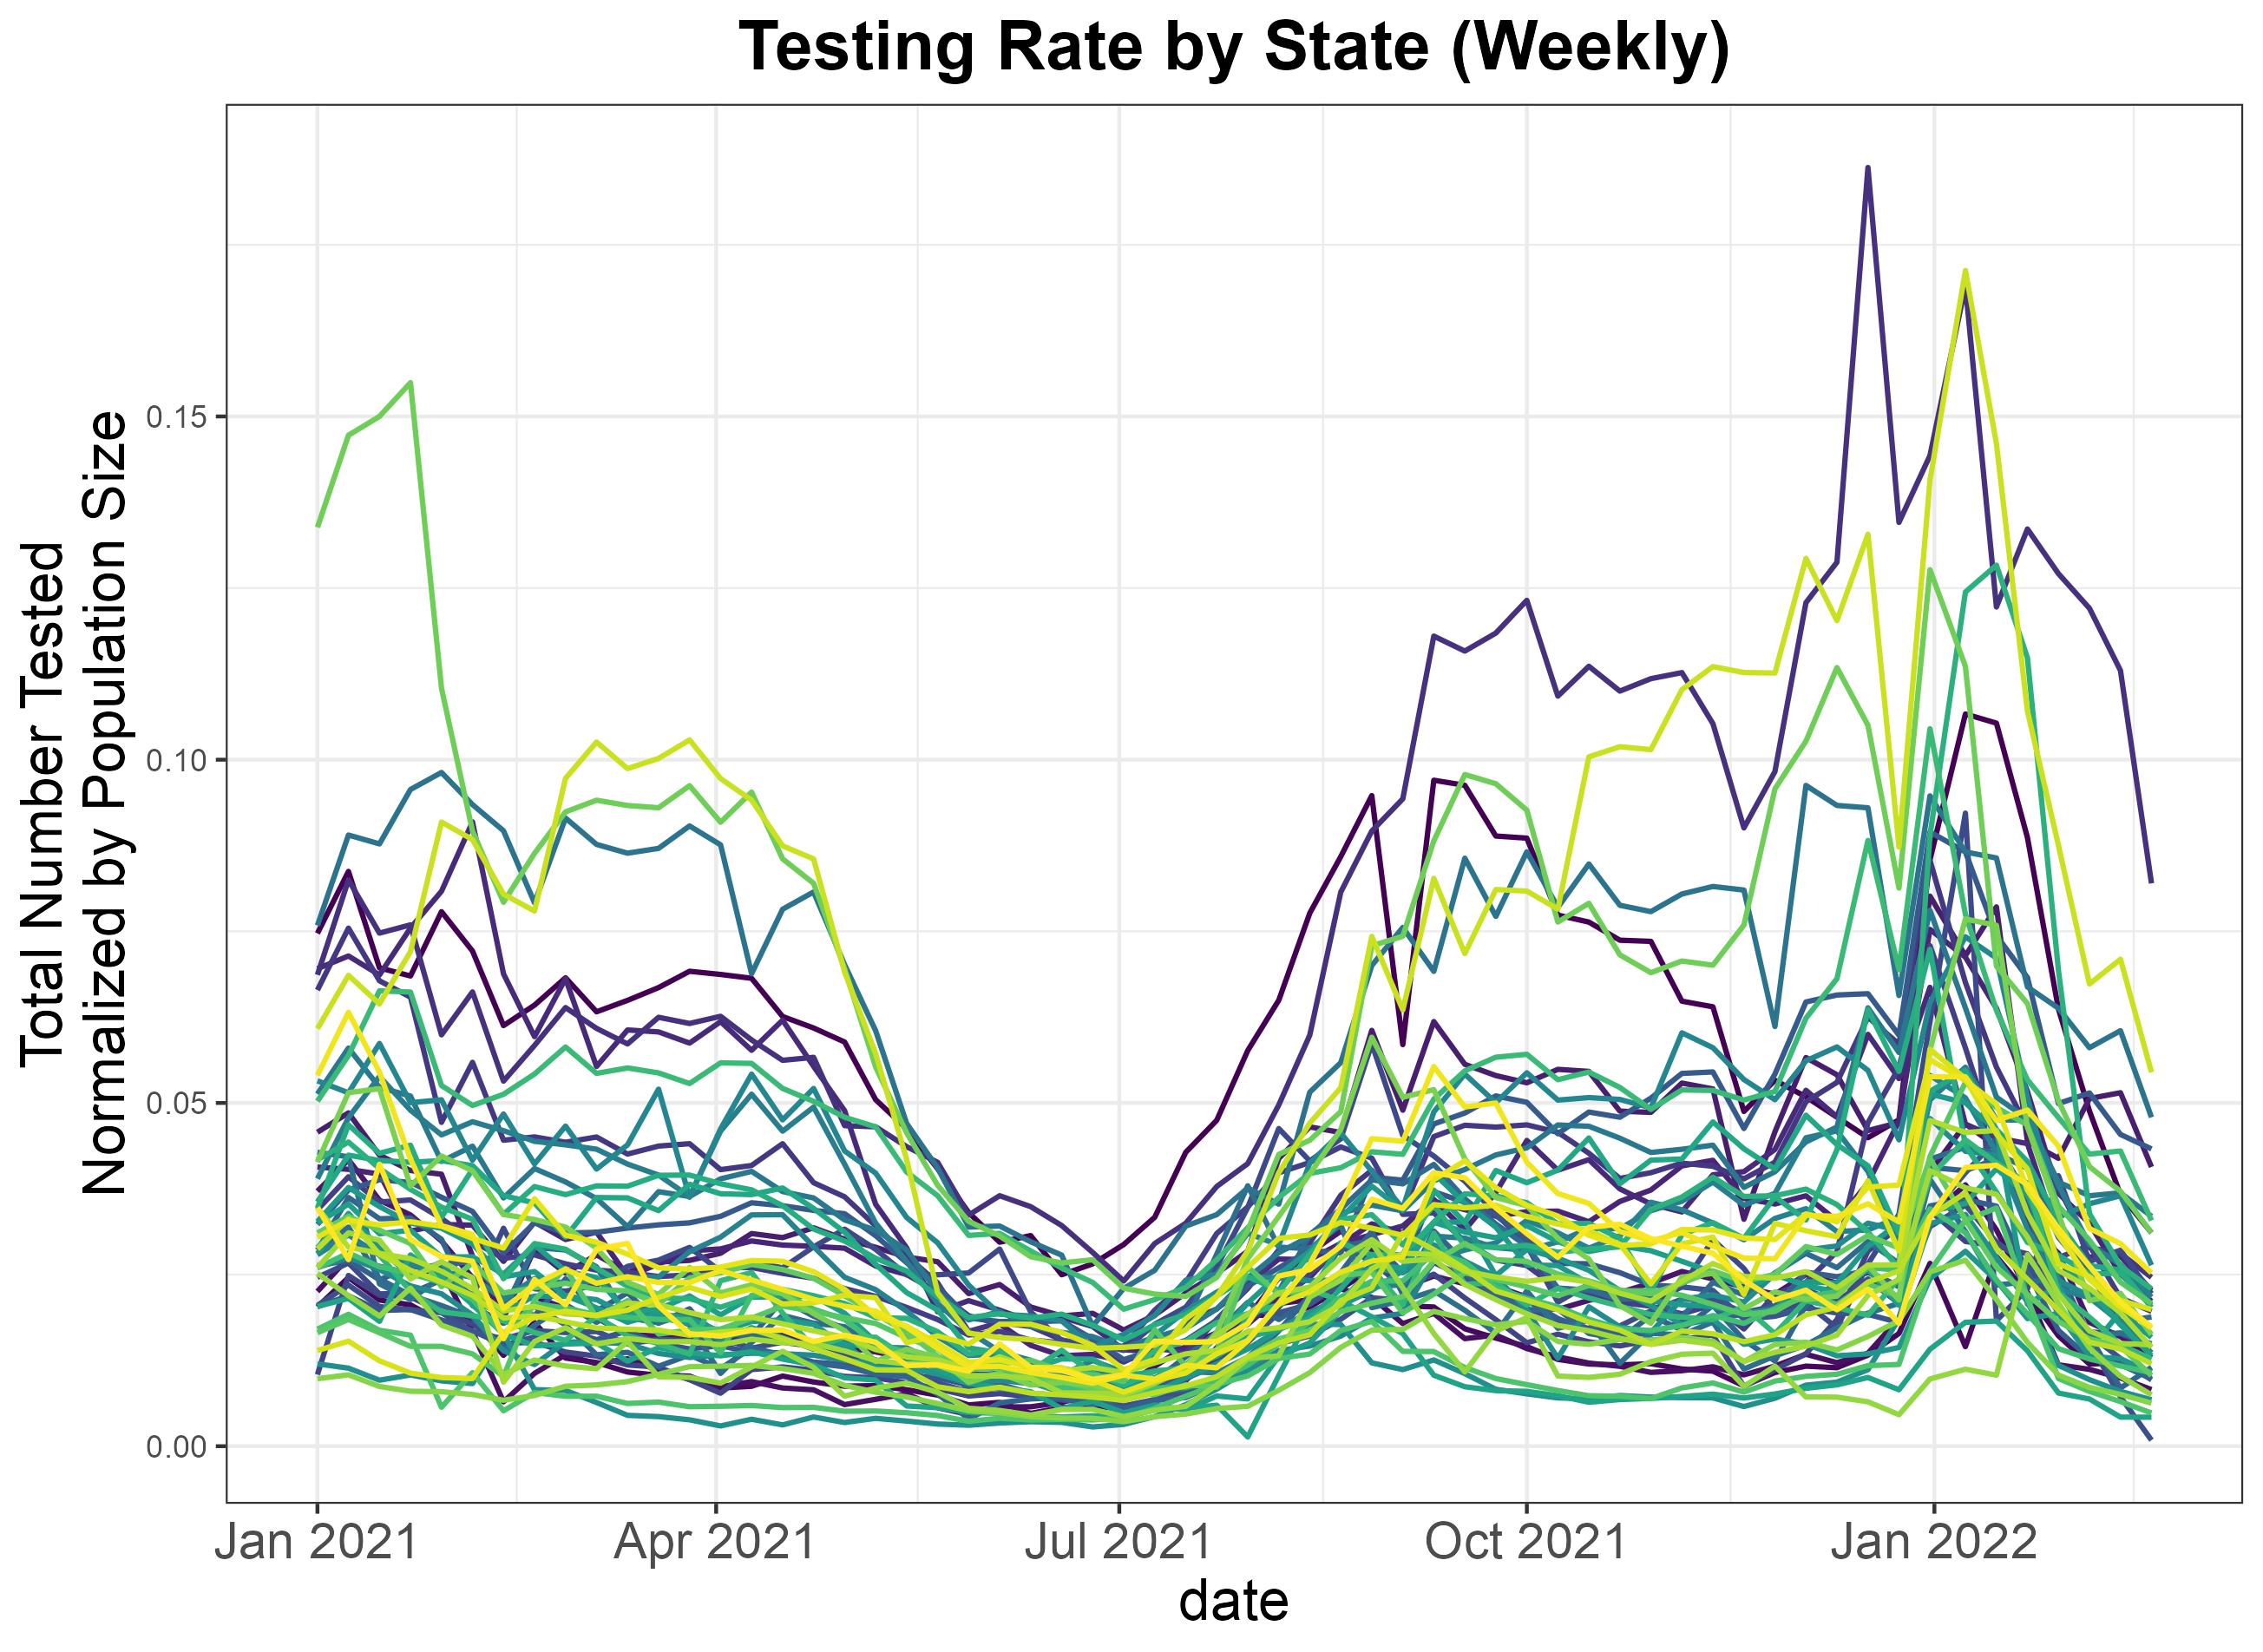
\includegraphics[width=0.9\linewidth]{./figure/testing_rate}

As we study the impact and transmission of SARS-CoV-2 as well as the efficacy of different interventions, we often turn to case counts for information. In this way, case counts form the basis for numerous types of analyses that inform our understanding of the pandemic. This means that bias in case counts due to unobserved infections can greatly impact our understanding of the pandemic.

One way testing rates can influence our understanding of COVID-19 is when we are seeking to make comparisons across different locations.

The government response to the pandemic has differed greatly by state, with a range of different policies and timelines as local governments weighted complex tradeoffs. The variability in state-level policies sparks several questions related to the consequences of these policies. Comparing case counts enables us to compare the impact of state-level management of the pandemic. For example, Kaufman \emph{et al.} used cumulative case counts to study the effect of state-level social distancing policies (Kaufman et al., 2021). At the county scale, Jiang \emph{et al.} evaluated the association between stay-at-home orders and daily incident cases (Jiang, Roy, Pollock, Shah, \& McCoy, 2022), and Kao \emph{et al.} looked at how the duration of multiple policy interventions -- face mask mandates, stay-at-home orders, and gathering bans -- affected monthly incidence (Kao et al., 2023).

The bias in case counts is particularly important for inference related to government interventions. With regard to government interventions, it is highly likely that lower testing resources may be related to less stringent policies in other respects. If this is the case, then lower cases may be observed in locations with less stringent policies as an artifact of inadequate testing rather than lower transmission. As a result, when we estimate the effect of a policy intervention based on observed cases, we may be underestimating the true impact.

Besides interventions, there has been substantial concern over the disparities in the impact of COVID-19. As a result, it is important to understand the relationship between various socioeconomic variables and case burden. Chen and Krieger showed a consistent monotonic relationship between the percent poverty and cumulative case burden at the zip-code tabulation area level in Illinois, with higher percent poverty associated with a higher case burden (J. T. Chen \& Krieger, 2021). Similarly, Karmakar \emph{et al.} showed in a cross-sectional analysis that for counties in the U.S., incident cases were associated with higher social vulnerability index (Karmakar, Lantz, \& Tipirneni, 2021). This social vulnerability index is defined by the CDC, and includes information from a collection of census variables related to poverty, unemployment, and racial and ethnic minority status.
Similar issues may arise when studying the effect of socioeconomic variables. Counties with higher social vulnerability (due to, for example, low economic resources) may also have lower testing resources, which may bias our comparisons to counties where testing is more adequate.

We also use cases to study the effect of vaccination at the population scale. Work in this area has been expansive. Harris showed an inverse relationship between cross-sectional COVID-19 incidence and county-level vaccination coverage during the Delta surge considering a sample of the counties with the largest population size (Harris, 2022), and Cuadros \emph{et al.} found a similar trend in counties across the United States (Cuadros et al., 2022). Nevertheless, as the virus has evolved, the relationship between transmission and case counts has shifted, particularly with the evolution of the highly transmissible Omicron variant. Mclaughlin \emph{et al.} found that there wasn't a relationship between the percentage of the population fully vaccinated and case counts, contrasting findings from other waves (McLaughlin, Wiemken, Khan, \& Jodar, 2022). However, they did find that higher booster uptake rates were associated with meaningful decreases in case counts, and higher vaccination rates and booster rates were both associated with decreases in COVID-19 mortality.

Beyond the efficacy of vaccines at the individual level, these studies also demonstrate that we can use case data to quantify the impact of vaccination efforts as a public health intervention. Coupled with information about genetic variants that are circulating, they also can extend our knowledge about the effect of this intervention across different phases of the pandemic.

Looking to the future, infection counts also may be informative as we better understand the impacts of long COVID-19\footnote{The syndrome goes by a number of names, including long-haul COVID-19, post-acute post-acute sequelae SARS-CoV-2 infection (PASC), among others.} on a population scale. There is increased concern over the poorly characterized but widespread phenomenon of lingering COVID-19 symptoms, which includes but is not limited to symptoms of fatigue, dyspnea, chest pain, and palpitation. The heterogeneity of presentations and definitions has complicated research on the syndrome, yet its impact has been pervasive. In light of this, the NIH has made the initiative Researching COVID to Enhance Recovery (RECOVER) Initiative to better understand and treat long COVID-19.

Infection counts are particularly relevant for the study of long COVID-19 at the population scale because, contrary to what we might expect, the severity of COVID-19 disease is not associated with the persistence of several symptoms, including anosmia, chest pain, cough, and palpitation (Dirican \& Bal, 2022). Since lingering symptoms can be problematic even with mild cases, trying to characterize the cumulative burden of COVID-19 through a proxy such as hospitalization counts would not capture the full impact.

Ultimately, COVID-19 case counts are a key metric that informs our understanding of the pandemic. Case numbers are interesting in themselves to quantify the reach of the pandemic across different time periods, and they are also the inputs to an extensive array of analyses that aid our understanding of public health interventions, disparities in the impact of the virus, and differences in the dynamics among circulating genetic variants. This underlies the importance of quantifying the underestimation of COVID-19 infections and how the extent of underestimation differs across time and space.

\hypertarget{overview-of-approach}{%
\chapter{Overview of Approach}\label{overview-of-approach}}

This work is based on the paper \emph{Substantial underestimation of SARS-CoV-2 infection in the United States} (Wu et al., 2020a). Wu \emph{et al.} considered a single time interval early in the pandemic, estimating the true number of infections as of April 18, 2020 at the state level. When we consider the estimates, we can look at both the estimates for total infections by state, but also the ratio of the estimated total cases to the observed cases. This enables us to think about the way case ascertainment varies by state, as we see in Figure
\ref{fig:originalfigwu}.
\begin{figure}
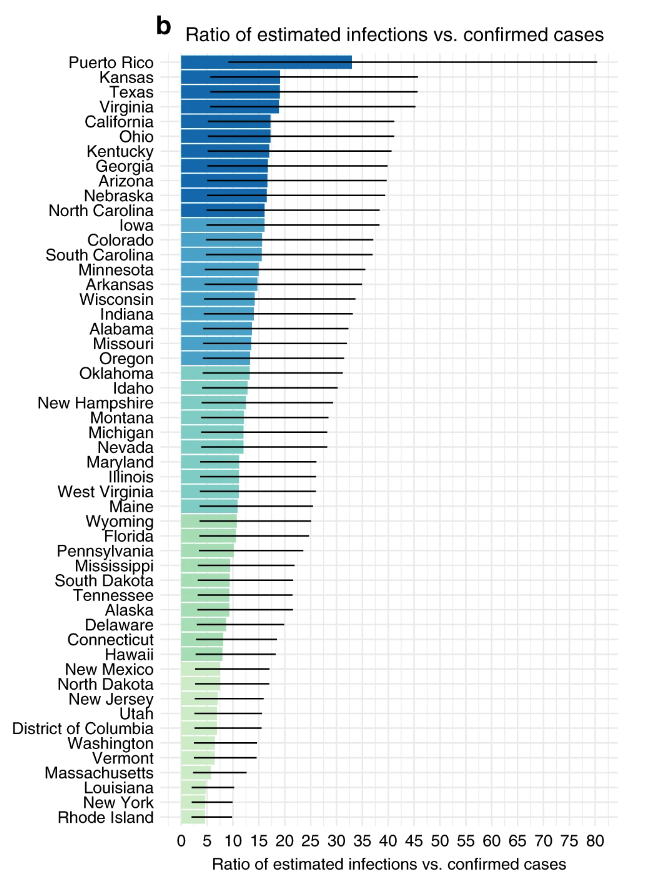
\includegraphics[width=0.5\linewidth]{./figure/figure_original_case_ratio} \caption{\label{fig:originalfigwu}Figure from Wu et al. (2020) showing the ratio of total estimated infections when accounting for imperfect diagnostic test accuracy and incomplete testing to the number of cases confirmed by a positive PCR test.}\label{fig:unnamed-chunk-7}
\end{figure}
The core idea of the approach is to break up the unobserved infections into unobserved infections among those with no or mild symptoms or those with moderate to severe symptoms. We denote this symptom status by an indicator variable, where \(S_1\) represents having moderate to severe symptoms and \(S_0\) represents having no or mild symptoms. In what follows, \(\text{test}_+\) denotes the event that an individual \emph{would} test positive if they were tested, not that they actually did. For example, \(\Pr(\text{test}_+|S_1,\text{untested})\) represents the probability a symptomatic untested individual would test positive if they were tested.

We let \(N^*\) denote the number of positive tests, to distinguish positive tests \(N^*\), which is affected by testing inaccuracy, from the number of active SARS-CoV-2 infections, \(N^+\).

Our first goal is to estimate the number of untested individuals who would test positive, \(N^*_{\text{untested}}\).

To estimate the number of untested individuals with moderate to severe COVID-19-like symptoms who would test positive untested population, we can take
\begin{align*}
N^*_{\text{untested},S_1} &=N_{\text{untested},S_1} \; \Pr(\text{test}_+ | S_1,\text{untested})\\
&=N_{\text{untested}} \; \Pr(S_1|\text{untested})) \; \Pr(\text{test}_+ | S_1,\text{untested}).
\end{align*}
Similarly, we can estimate the asymptomatic (or mild) infections among the untested population as
\begin{align*}
N^*_{\text{untested},S_0} &=N_{\text{untested},S_0} \; \Pr(\text{test}_+ | S_0,\text{untested})\\
&=N_{\text{untested}} \Pr(S_0|\text{untested}) \; \Pr(\text{test}_+ | S_0,\text{untested})\\
&=N_{\text{untested}}(1-\Pr(S_1|\text{untested})) \; \Pr(\text{test}_+ | S_0,\text{untested}).
\end{align*}
Taking the sum of the positive tests among gives us the total:

\[N^*_{\text{untested}} = N^*_{\text{untested},S_1} + N^*_{\text{untested},S_0}.\]
This allows us to obtain the estimated number of positive tests as

\[N^* = N^*_{\text{untested}} +N^*_{\text{tested}},\]
where \(N^*_{\text{tested}}\) is the number of positive tests in a given location.

At this point, we can apply a simple epidemiology formula to that corrects for the test specificity and sensitivity of the diagnostic test (Rothman, Greenland, \& Lash, 2008). Denoting the sensitivity \(S_e\) and specificity \(S_p\), this formula is given by

\[\text{Number Truly Positive} = \dfrac{N^+ - (1-S_p) \times N}{S_e+S_p-1}.\]

The uncertainty inherent in this estimation process is in the quantities \(\Pr(S_1|\text{untested})\), \(\Pr(\text{test}_+| S_1,\text{untested})\), and \(\Pr(\text{test}_+ | S_0,\text{untested})\).

It is particularly difficult to think about how we would estimate \(\Pr(\text{test}_+ | S_0,\text{untested})\) or \(\Pr(\text{test}_+ | S_1,\text{untested})\) directly because there is a lack of data on these quantities.

Instead, we define random variables to relate the symptomatic and asymptomatic test positives to the observed positivity rate \(\Pr(\text{test}_|\text{tested})\).

In particular, we define
\begin{align*}
\alpha &= \dfrac{\Pr(test + |S_1, \text{untested})}{\Pr(\text{test}_+ | \text{tested})}\\
\beta  &= \dfrac{\Pr(test + |S_0, \text{untested})}{\Pr(\text{test}_+ | \text{tested})}.
\end{align*}
We can think of \(\alpha\) and \(\beta\) as variables that correct the observed test positivity rate to estimate the test positivity rate among the symptomatic and asymptomatic partitions of the population respectively.

We can think of \(\alpha\) as the correction factor for estimating \(\Pr(+|S_1,\text{untested})\) from the test positivity \(\Pr(\text{test}_+ |\text{tested})\).

We can define \(\beta\) analogously for the asymptomatic case, where
\[\beta =  \dfrac{\Pr(\text{test}_+ |S_0, \text{untested})}{\Pr(\text{test}_+ | \text{tested})},\]
so we have \(\Pr(\text{test}_+ |S_0, \text{untested}) = \beta \; \Pr(\text{test}_+ | \text{tested})\).

This formulation enables us to estimate \(\Pr(\text{test}_+ |S_0, \text{untested})\) and \(\Pr(\text{test}_+ |S_1, \text{untested})\) with information from the observed test positivity rate among the tested population, which means it can reflect differences in transmission dynamics by the location and time interval considered.

We expect \(\alpha\) to be higher than \(\beta\) to reflect that the test positivity rate among the asymptomatic untested population is lower than the symptomatic untested population. The specification of these distributions is discussed in greater detail in the {[}Definition of Prior Distributions for the Bias Parameters {]} section.

Because of the uncertainty around \(\alpha\) and \(\beta\), it is useful to relate these parameters to the asymptomatic rate of the virus, \(\Pr(S_0|\text{test}_+, \text{untested})\). Due to the importance of asymptomatic transmission to controlling the pandemic, the asymptomatic rate has been an area of substantial interest. This has led to extensive studies on the topic, including multiple meta-analyses summarizing these results (Ma et al., 2021a; Sah et al., 2021a).

We can represent the relationship between \(\theta = \{ \alpha, \beta, \Pr(S_1|\text{untested})\}\) and \(\phi = \{\; \Pr(S_0|\text{test}_+, \text{untested})\;\}\) by the deterministic function
\(M: \theta \to \phi\) for \(\theta = \{\Pr(S_1|\text{untested}), \alpha, \beta \}\) and \(\phi = \Pr(S_0|test +,\text{untested})\) defined as:
\[\Pr(S_0|\text{test}_+, \text{untested}) = \dfrac{\beta(1 - \Pr(S_1|\text{untested}))}{\beta(1-\Pr(S_1|\text{untested})) + \alpha \Pr(S_1|\text{untested})}.\]

When we have prior knowledge about the distributions of the inputs and output of a deterministic function, we can use \protect\hyperlink{meld}{Bayesian melding} to generate constrained distributions for the inputs and outputs that are in concordance with one another. In essence, this approach considers the distinct distributions we have for \(\phi\): the distribution informed by previous literature on the asymptomatic rate, and the distribution formed by evaluating \(M\) at values of \(\theta\). We can combine these distributions with logarithmic pooling to yield a constrained distribution for \(\phi=\Pr(S_0|\text{test}_+, \text{untested})\), and then can approximate the inverted distribution to obtain constrained distributions for the inputs \(\theta = \{\Pr(S_1|\text{untested}), \alpha, \beta \}\).

We can summarize this process in Figure \ref{fig:diagram}. We repeat this process for every geographic unit (a state or county) and time interval (a 2 week interval).
\begin{figure}

{\centering 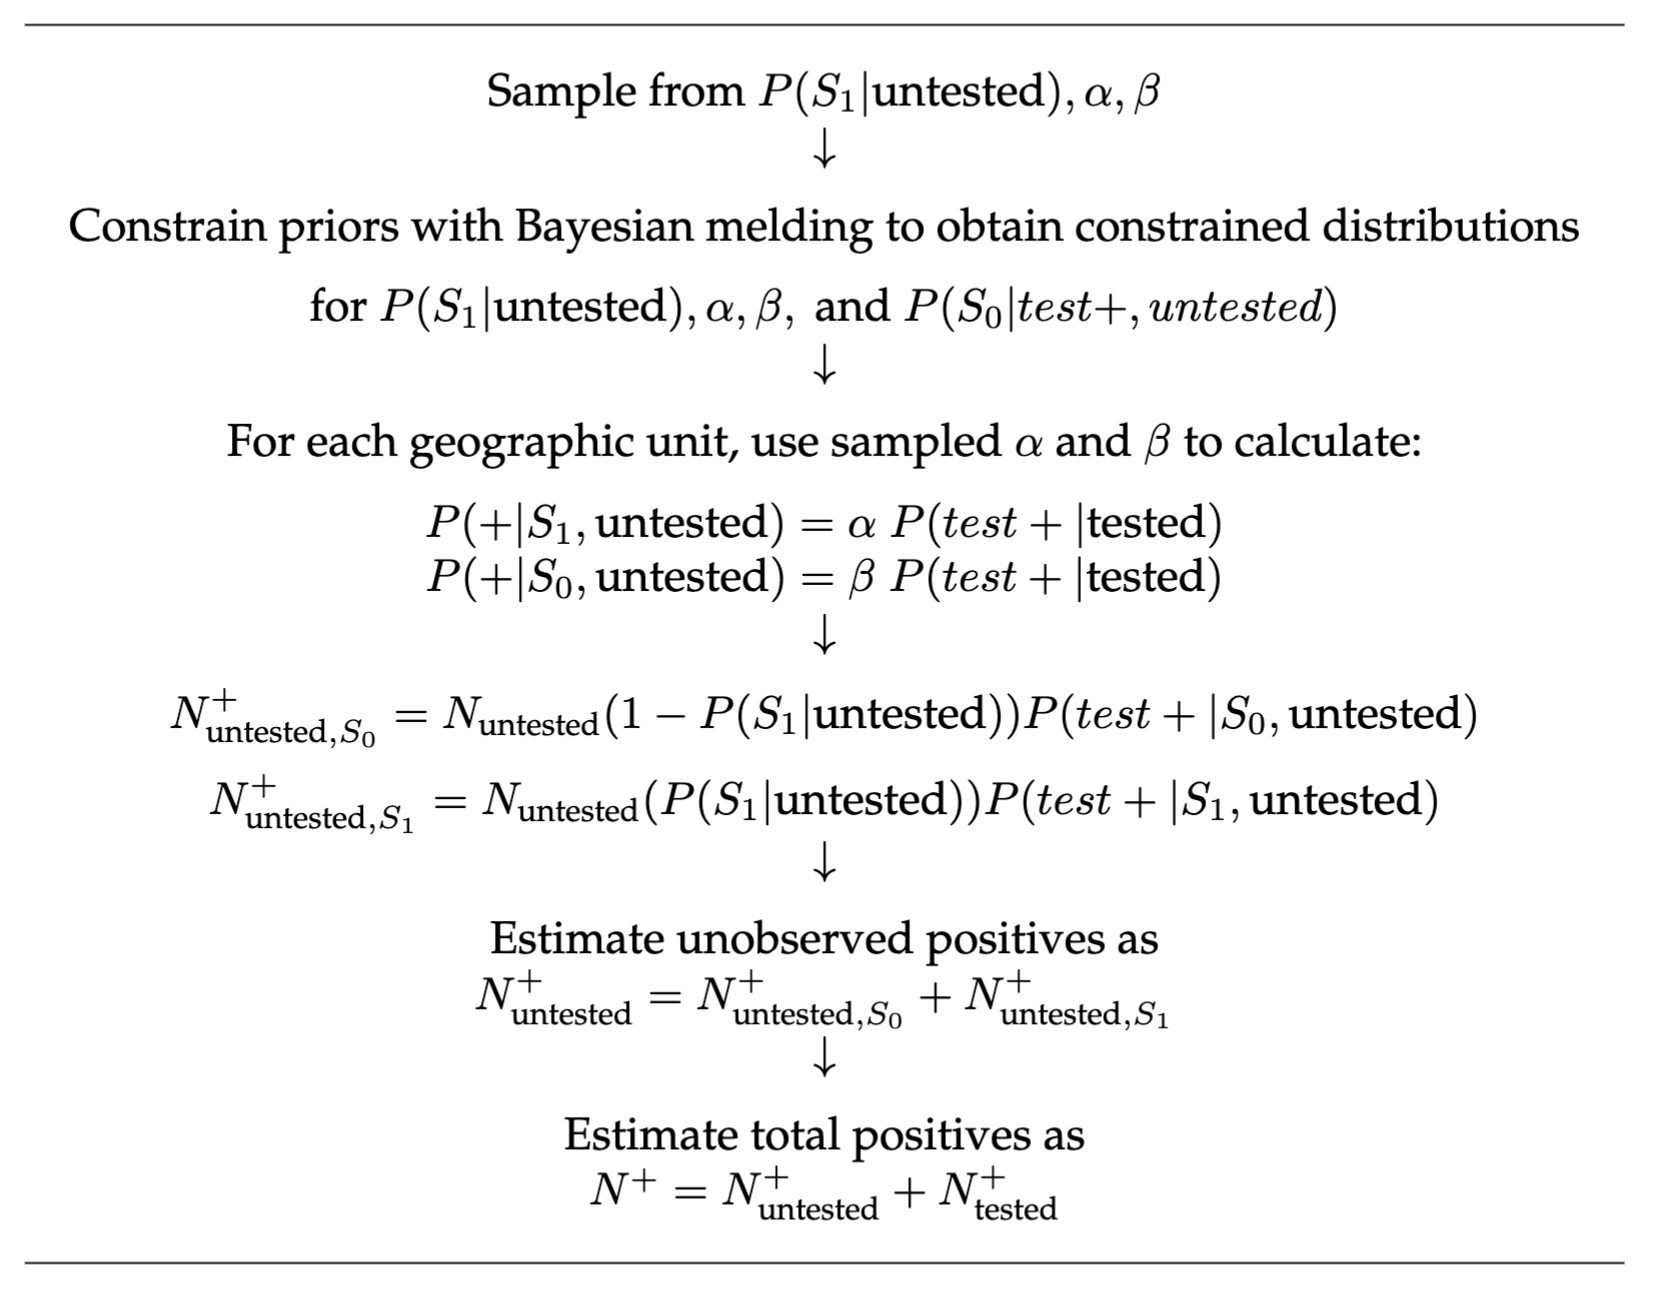
\includegraphics[width=1\linewidth]{./figure/analysis_diagram} 

}

\caption{\label{fig:diagram}Implementation of probabilistic bias analysis.}\label{fig:unnamed-chunk-8}
\end{figure}
We divide the time period into 2-week intervals specifically due to the duration of test positivity, which is about two weeks on average (Kojima, Roshani, \& Klausner, 2022; Mallett et al., 2020). Because
\[ \text{Prevalence} = (\text{Incidence Rate}) \times (\text{Average Duration of Disease}), \]

prevalent infections and incident infections are approximately equivalent on the two-week time scale, which enables us to think of our estimates for each two-week period as incident infections.

With the implementation of the implementation of Wu et al. (2020b), \(\alpha, \beta, \text{and} \Pr(S_1|\text{untested})\) were assumed to be independent and identically distributed across states. However, because we are considering a wider time interval over all of 2021 and into early 2022, it makes sense to vary these parameters by time and location. Due to the availability of data to inform \(\beta\) and \(\Pr(S_1|\text{untested})\), we allow these parameters to vary by time and location, as discussed further in \protect\hyperlink{defpriors}{Definition of Prior Distributions}.

When we allow \(\beta\) and \(\Pr(S_1|\text{untested})\) to vary over time and location, rather than implementing Bayesian melding once and using the same melded distribution for each time interval, we must implement melding for each time interval separately.

\hypertarget{background}{%
\chapter{Background}\label{background}}

\hypertarget{probabalistic-bias-analysis}{%
\section{Probabalistic Bias Analysis}\label{probabalistic-bias-analysis}}

Often the focus of quantifying error about an effect estimate focuses on random error rather than the systematic error. For example, typical frequentist confidence intervals are frequent in medical and epidemiological literature, although they have faced rising criticism (Greenland et al., 2016). These confidence intervals quantify the fraction of the times we expect the true value to fall in this interval under the assumption that our model is correct. That is, if we ran an experiment 100 times and computed the effect size each time, we would expect the 95\% confidence interval to contain the true value to 95 of those times, on average. Neyman stressed this in his original publication formalizing the concept of a confidence interval in 1937 (Neyman, 1937). The nuance that the confidence interval is not the probability that the true value falls within this interval, however, is often lost in the discussion of results, in part because the true meaning of a confidence interval is less intuitive.

The aim of quantitative bias analysis is to estimate systematic error to give a range of possible values for the true quantity of interest. In this sense, it is a type of sensitivity analysis. It can be used to estimate various kinds of biases, from misclassification, as is implemented in this work, as well as selection bias and unmeasured confounding (Petersen, Ranker, Barnard-Mayers, MacLehose, \& Fox, 2021). Often, the goal of performing such an analysis is to see how these sources of bias affect our estimates; in particular, under what situations of bias the observed effect would be null.

There are multiple different forms of bias analysis (Lash, Fox, \& Fink, 2009). The most simple case, simple bias analysis, is correcting a point estimate for a single source of error. Multidimensional bias analysis extends this to consider sets of bias parameters, but still provides a corrected point estimate rather than a range of plausible estimates. Probabilistic bias analysis, meanwhile, defines probability distributions for bias parameters to generate a distribution of corrected estimates by repeatedly correcting estimates for bias under different combinations of the parameter values. Then, via Monte Carlo we obtain a distribution of corrected estimates that reflect the corrected values under different scenarios of bias, that is, under different combinations of the bias parameters. This can give us a better idea for the extent of uncertainty about the corrected estimates, although this uncertainty does depend on the specification of the bias parameter distributions. Inherent in bias analysis is the dependence of our results on the specification of bias parameters, which reflect what is known from available data, literature, or theory on the extent of bias that may occur. There is uncertainty about how we define these distributions or values; otherwise, if the precise values of the bias parameters were known, we could simply correct the estimates and probabilistic bias analysis would not be useful.

Although some forms of probabilistic bias analysis can be applied to summarized data, for example, frequencies in a contingency table, the methods are most often implemented with unsummarized data in its original form, as implemented here.

In choosing specific distributions for the bias parameters, different specifications may yield density functions where most of the density is within a similar interval, which means the choice of the specific distribution will not be sensitive to the particular choice of density.

\hypertarget{background-for-the-approach}{%
\section{Background for the Approach}\label{background-for-the-approach}}

The Bayesian melding approach was proposed by Poole et al. (Poole \& Raftery, 2000).

This approach enables us to account for both uncertainty from inputs and outputs of a deterministic model. The initial motivation for the approach was to study the population dynamics of whales in the presence of substantial uncertainty around model inputs for population growth (Poole \& Raftery, 2000). However, the framework provided by Poole et al.~can applied in any circumstance where we have uncertainty around some quantities \(\theta\) and \(\phi\) where there is a deterministic function \(M:\theta \to\phi\). Due the utility of Bayesian melding in various contexts, since this deterministic model \(M\) could take on a wide range of forms, the approach has since been applied in various fields, including urban simulations (Ševčíková, Raftery, \& Waddell, 2007), ecology (Robson, 2014), and infectious disease (Powers et al., 2011).

Let \(M: \theta \to \phi\) be the deterministic model defined by the function relating a vector of input parameters \(\theta\) to an output vector \(\phi\), and suppose we have a prior on \(\theta\) denoted \(f_\theta(\theta)\) and a prior on \(\phi\) denoted \(f_\phi^{direct}(\phi)\).

However, note that we actually have two distinct priors on \(\phi\). There is the prior formed by the distribution induced on \(\phi\) by the prior for \(\theta\) and the function \(M\), where we denote this induced prior \(f_\phi^{induced}(\phi)\). Generally, these priors are based on different sources of information.

If \(M^{-1}\) exists, we can write this induced prior \(f_\phi^{induced}(\phi) = f_\theta(M^{-1}(\phi)) |J(\phi)|\)\footnote{In the continuous case we need to multiply by \(|J(\phi)|\), but not in the discrete case (Blitzstein \& Hwang, 2019).}. This result follows from the fact \(M(\theta) = \phi\), so we apply a change of variables to obtain the distribution of \(\phi\) from the distribution of \(M(\theta)\).

In practice, \(M^{-1}\) rarely exists exists since \(\theta\) is often of higher dimensionality then \(\phi\), in which cases \(M\) is not invertible. This means we generally approximate \(f_\phi^{induced}\) without acquiring its analytical form.

In addition to this induced prior, we have the prior \(f_\phi^{direct}(\phi)\), which does not involve \(M\) nor the inputs \(\theta\). Since these priors are based on different sources of information and may reflect different uncertainties, often it useful to use both sources of information to inform our estimates. To do so, we need to combine the distributions for \(f_\phi^{induced}\) and \(f_\phi^{direct}\) to create a pooled distribution.

Multiple pooling strategies exist for distinct distributions, but one requirement for a Bayesian analysis is that the distribution should be independent of the order in which the prior is updated and the combining of the prior distribution. That is, updating the prior distributions using Bayes' theorem and then combining distributions should yield the same result as combining distributions and then updating this combined distribution; pooling methods that have this property are deemed externally Bayesian. Logarithmic pooling has been shown to be externally Bayesian under some conditions, which are likely to hold in most settings. Furthermore, logarithmic pooling has actually been shown to be the only pooling method where this holds (Genest, McConway, \& Schervish, 1986). For this reason, Poole \emph{et al.} recommend proceeding with logarithmic pooling for Bayesian melding.

The logarithmically pooled prior for \(\phi\) by pooling \(f_\phi^{induced}\) and \(f_\phi^{direct}\) is

\[f_\phi^{pooled} (\phi) = t(\boldsymbol{\alpha}) (f_\phi^{induced}(\phi))^{\alpha} (f_\phi^{direct}(\phi))^{1-\alpha}.\]

The pooling weights are given by \(\boldsymbol{\alpha} = (\alpha, \;\;1-\alpha)\) where \(\alpha \in [0,1]\), and \(t(\boldsymbol{\alpha})\) is the normalizing constant. Commonly, a choice of \(\alpha = 0.5\) is used to give the priors equal weight. In this case, logarithmic pooling may be referred to as geometric pooling since it is equivalent to taking a geometric mean.

If \(M\) is invertible, we can obtain the contrained distributions for the model inputs by simply inverting \(M\). However, \(M\) is rarely invertible, so we have to think about how to proceed in the noninvertible case.

\hypertarget{simple-discrete-example}{%
\subsection{Simple Discrete Example}\label{simple-discrete-example}}

To get intuition for a valid strategy Poole et al.~recommend, we consider a mapping \(M: \theta \to \phi\) for \(\theta \in \mathbb{R}\) and \(\phi \in \mathbb{R}\)
defined as follows (Figure \ref{fig:dex}). Note the choice of \(f_\theta,f_\phi^{direct}\) does not matter here as long as they are valid densities.
\begin{multicols}{2}
\begin{figure}

{\centering 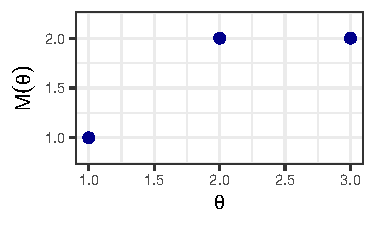
\includegraphics[width=1\linewidth]{thesis_files/figure-latex/unnamed-chunk-12-1} 

}

\caption{\label{fig:dex}A simple discrete example where $M$ is not invertible.}\label{fig:unnamed-chunk-12}
\end{figure}
\columnbreak
\begin{table}[H]
\centering
\begin{tabular}[t]{r|r|r|r}
\hline
$\theta$ & $f_\theta(\theta)$ & $M(\theta)=\phi$ & $f_\phi^{direct}(\phi)$\\
\hline
1 & 0.3 & 1 & 0.4\\
\hline
2 & 0.2 & 2 & 0.6\\
\hline
3 & 0.5 & 2 & 0.6\\
\hline
\end{tabular}
\end{table}
\end{multicols}
We see that \(M\) is not invertible since \(\theta=1\) and \(\theta = 2\) both map to \(\phi=2\), which implies the inverse \(M^{-1}\) would not be well defined.

We can generate a sample from the density \(f_\phi^{induced}\) by sampling from \(f_\theta\) and computing \(M(\theta)\).

So we have
\begin{align*}
f_\phi^{induced}(1) &= f_{\theta}(1) = 0.3 & \text{ (since $\theta = 1$ maps $\phi = 1$) } \\
f_\phi^{induced}(2) &= f_{\theta}(2) +  f_{\theta}(3) = 0.2 + 0.5=  0.7 & \text{ (since $\theta = 2$ and $\theta=3$ both map to $\phi = 2$) }
\end{align*}
Then, we can compute the logarithmically pooled pooled prior with \(\alpha=0.5\) by taking \(f_\phi^{induced}(\phi)^{\alpha} f_\phi^{direct}(\phi)^{1-\alpha}\).

This gives us
\begin{align*}
f_\phi^{induced}(\phi)^{\alpha} f_\phi^{direct}(\phi)^{1-\alpha} &= (0.3)^{0.5}(0.4)^{0.5} = 0.3464\\
f_\phi^{induced}(\phi)^{\alpha} f_\phi^{direct}(\phi)^{1-\alpha} &= (0.7)^{0.5}(0.6)^{0.5} = 0.6481.
\end{align*}
To make this a valid density, however, these probabilities must sum to 1, so we renormalize by dividing by (0.3464 + 0.6481). Denoting the pooled prior in phi-space as \(f_\phi^{pooled}(\phi)\), this gives us
\begin{align*}
f_\phi^{pooled}(1) &= \frac{ 0.3464  }  { 0.3464 + 0.6481 } = 0.3483 \\
f_\phi^{pooled}(2) &= \dfrac{ 0.6481 } { 0.3464 + 0.6481}  =0.6517.
\end{align*}
We summarize these results and compare \(f_\phi^{induced}, f_\phi^{direct}\), and \(f_\phi^{pooled}\) in Figure \ref{fig:comp}.
\begin{multicols}{2}
\begin{table}[H]
\centering
\begin{tabular}[t]{r|r|r|r}
\hline
$\phi$ & $f_\phi^{direct}(\phi)$ & $f_\phi^{induced}(\phi)$ & $f_\phi^{pooled}(\phi)$\\
\hline
1 & 0.4 & 0.3 & 0.3483\\
\hline
2 & 0.6 & 0.7 & 0.6517\\
\hline
\end{tabular}
\end{table}
\columnbreak
\begin{figure}

{\centering 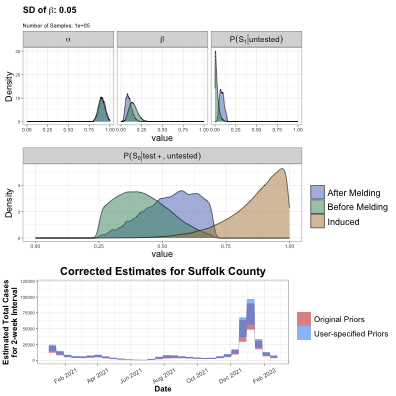
\includegraphics[width=1\linewidth]{thesis_files/figure-latex/unnamed-chunk-15-1} 

}

\caption{\label{fig:comp}}\label{fig:unnamed-chunk-15}
\end{figure}
\end{multicols}
However, we also want the pooled prior on the inputs \(\theta\), that is, \(f_\theta^{pooled}(\theta)\).

Poole et al.~reasoned as follows. Since \(M\) uniquely maps \(\theta=1\) to \(\phi =1\), the probability that \(\theta=1\) should be equal to the probability \(\phi = 1\). That is, we should have \(f_\theta^{pooled}(1) = f_\phi^{pooled}(1)\).

However, the relationship for \(\theta=2\) or \(\theta=3\) to \(\phi\) is not one to one. Since \(M(2)=2\) and \(M(3)=2\), the sum of the probabilities for \(\theta=1\) and \(\theta=2\) should be equal to that for \(\phi=2\), that is, \(f_\theta^{pooled}(2) + f_\theta^{pooled}(3) = f_\phi^{pooled}(2) = 0.6517\).

The challenge here is how we divide the probability for \(f_\phi^{pooled}(2)\), which is defined, among \(f_\theta^{pooled}(2)\) and \(f_\theta^{pooled}(3)\). The prior for \(\phi\) yields no information to assist in this choice, because knowing which value \(\phi\) takes on does not give us any information about whether \(\theta=2\) or \(\theta=3\). Thus, the information we have about \(\theta\) must be taken from \(f_\theta(\theta)\).

That is, we can assign a probability for \(f_\theta^{pooled}(2)\) by considering the probability that \(\theta = 2\) relative to the probability \(\theta =3\), computing

\[f_\theta^{pooled}(2) = f_\phi^{pooled}(2) \Big( \frac{f_\theta(2)}{f_\theta(2) + f_\theta(3)}\Big).\]

That is, if the probability \(\theta\) takes on the value \(2\) is lower in this case than the probability \(\theta=3\) which we know from the prior on \(\theta\), \(f_\theta(\theta)\), then the pooled prior on \(\theta\), \(f_\theta^{pooled}(2)\), should reflect this.

Using this reasoning, we have
\begin{align*} f_\theta^{pooled}(2) &= (0.7) \frac{0.2}{0.2+0.5} = 0.1862\\
f_\theta^{pooled}(3) &= (0.7) \frac{0.5}{0.2+0.5} = 0.4655.
\end{align*}
The result in this simple example, using \(f_\theta(\theta)\) to determine how to distribute the probability for values of \(\phi\) where multiple \(\theta\) map to \(\phi\), can be used to derive general formulas to compute \(f_\theta^{pooled}(\theta)\) for discrete and continuous distributions (Poole \& Raftery, 2000).

\hypertarget{general-solution-for-the-discrete-case}{%
\subsection{General Solution for the Discrete Case}\label{general-solution-for-the-discrete-case}}

Denote the possible values of \(\theta\) as \(A_1, A_2, \dots\), the possible values of \(\phi\) as \(B_1, B_2, \dots\), and a mapping \(m: \mathbb{N} \to \mathbb{N}\) such that \(M(A_i) = B_{m(i)}\) and \(C_j = M^{-1}(B_j) = \{A_i : M(A_i) = B_j\}\). Then

\[f_\theta^{pooled}(A_i) = f_\phi^{pooled}(B_{m(i)}) \left( \frac{f_\theta(A_i)}{f_\phi^{induced}(B_{m(i)})} \right).\]

\hypertarget{general-solution-for-the-continuous-case}{%
\subsection{General Solution for the Continuous Case}\label{general-solution-for-the-continuous-case}}

We denote \(B = M(A) = \{M(\theta) : \theta \in A \}\) and \(C = M^{-1}(B) = \{\theta: M(\theta) \in B \}\).

Then

\[
f_\phi^{pooled} (M(\theta)) =t({\alpha}) f_\theta(\theta) \left( \frac{f_\phi^{direct}(M(\theta))}{f_\phi^{induced}(M(\theta))} \right)^{1-\alpha} \tag{2}
\]
where \(t({\alpha})\) is a renormalizing constant for the choice of \(\alpha\).

\hypertarget{implementation-through-the-sampling-importance-resampling-algorithm}{%
\subsection{Implementation through the Sampling-Importance-Resampling Algorithm}\label{implementation-through-the-sampling-importance-resampling-algorithm}}

We can obtain the pooled distributions \(f^{pooled}_\theta\) and \(f^{pooled}_\phi\) by using the Sampling-Importance-Resampling Algorithm.

The steps are as follows.
\begin{enumerate}
\def\labelenumi{\arabic{enumi}.}
\tightlist
\item
  We draw \(\theta\) from its prior distribution \(f_\theta(\theta)\).
\item
  For every \(\theta_i\) we compute \(\phi_i = M(\theta_i)\) to obtain a sample from the induced distribution.
\item
  Since the density \(f_\phi^{induced}(\phi)\) is unlikely to have an analytical form, we can compute it via a density approximation such as kernel density estimation.
\item
  Construct weights proportional to the ratio of the prior on \(\phi\) evaluated at \(M(\theta_i)\) to the induced prior \(f_\phi^{induced}\) evaluated at \(M(\theta_i)\). If a likelihood \(L_1(\theta)\) for the inputs and \(L_2(\phi)\) is available, the weights are
  \[w_i = \left( \frac{f_\phi^{direct}(M(\theta_i))}{f_\phi^{induced}(M(\theta_i))} \right)^{1-\alpha}L_1(\theta_i) \; L_2(M(\theta_i)).\]
  However, in this work, no likelihood is available for the variables of interest, so the likelihood is left out of the weights, leaving us with
  \[w_i = \left( \frac{f_\phi^{direct}(M(\theta_i))}{f_\phi^{induced}(M(\theta_i))} \right)^{1-\alpha}.\]
\item
  Sample \(\theta\) and \(\phi\) from step (1) with probabilities proportional to the weights from (4).
\end{enumerate}
\newpage

\hypertarget{meld}{%
\section{Bayesian Melding Applied to COVID-19 Misclassification}\label{meld}}

~~~In this work, we can relate the inputs \(\theta = \{P(S_1|\text{untested}), \alpha, \beta \}\) and \(\phi = P(S_0|\text{test}_+,\text{untested})\) by the deterministic model \(M: \theta \to \phi\) given by \(P(S_0|\text{test}_+, \text{untested}) = \dfrac{\beta(1 - P(S_1|\text{untested}))}{\beta(1-P(S_1|\text{untested})) + \alpha P(S_1|\text{untested})}.\) The derivation of \(M\) is in the \protect\hyperlink{derivation}{following section.}

Now, we have two distributions on \(\phi\): the distribution based on data on the asymptomatic rate of infection of COVID-19, and the distribution formed by taking \(M(\theta)\) where \(\theta\) represents the values from the defined distributions of \(\alpha,\beta,\) and \(P(S_1|\text{untested}\). With Bayesian melding, we pool these distributions using logarithmic pooling, and then implement the sampling-importance-resampling algorithm to obtain constrained distributions of the inputs \(\theta\) that are in accordance with information about the asymptomatic rate of the virus.

Due to the uncertainty around our definitions of \(\alpha\) and \(\beta\), it is particularly useful to leverage the information we have about the asymptomatic rate of the virus \(P(S_0|\text{test}_+,\text{untested})\) because a large collection of studies has been published in this area. In a meta-analysis pooling data from 95 studies, the pooled estimate among the confirmed population that was asymptomatic was 40.50\% {[}95\% CI, 33.50\%-47.50\%{]} (Ma et al., 2021b). Another meta-analysis including 350 studies estimated the asymptomatic percentage to be 36.9\% {[}95\% CI: 31.8 to 42.4\%{]}, and, when restricting to screening studies, 47.3\% (95\% CI: 34.0\% -61.0\%) (Sah et al., 2021b).

This means we have two priors on the asymptomatic rate \(\phi\), that by taking \(M(\theta)\) for sampled values of \(\theta\), denoted \(f_\phi^{induced}\) in the previous section, and that based on data about the asymptomatic rate, \(f_\phi^{direct}\).

\newpage

\hypertarget{distribution-of-theta-alpha-beta-ps_1textuntested}{%
\subsection{\texorpdfstring{Distribution of \(\theta = \{\alpha, \beta, P(S_1|\text{untested}) \}\)}{Distribution of \textbackslash theta = \textbackslash\{\textbackslash alpha, \textbackslash beta, P(S\_1\textbar\textbackslash text\{untested\}) \textbackslash\}}}\label{distribution-of-theta-alpha-beta-ps_1textuntested}}

First, we obtain a sample \(\theta_1, \theta_2, \dots, \theta_k\) from \(\theta\) (Figure \ref{fig:theta}).
\begin{figure}

{\centering 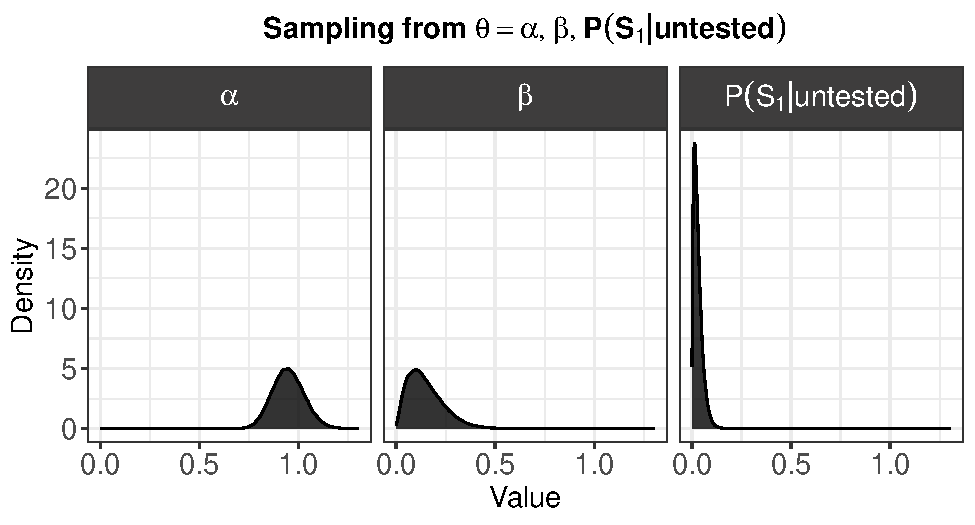
\includegraphics[width=1\linewidth]{thesis_files/figure-latex/create theta.png-1} 

}

\caption{\label{fig:theta}}(\#fig:create theta.png)
\end{figure}
\hypertarget{direct-prior-and-induced-prior-distributions-for-ps_0texttest_textuntested}{%
\subsection{\texorpdfstring{Direct Prior and Induced Prior Distributions for \(P(S_0|\text{test}_+,\text{untested})\)}{Direct Prior and Induced Prior Distributions for P(S\_0\textbar\textbackslash text\{test\}\_+,\textbackslash text\{untested\})}}\label{direct-prior-and-induced-prior-distributions-for-ps_0texttest_textuntested}}

Then, taking \(M(\theta)\), we can compute the induced distribution \(f_\phi^{induced}(M(\theta))\) and compare it to our prior on \(\phi\) from meta-analyses on the asymptomatic rate, \(f_\phi^{direct}(\phi)\) (\ref{fig:prior-induced}).
\begin{figure}

{\centering 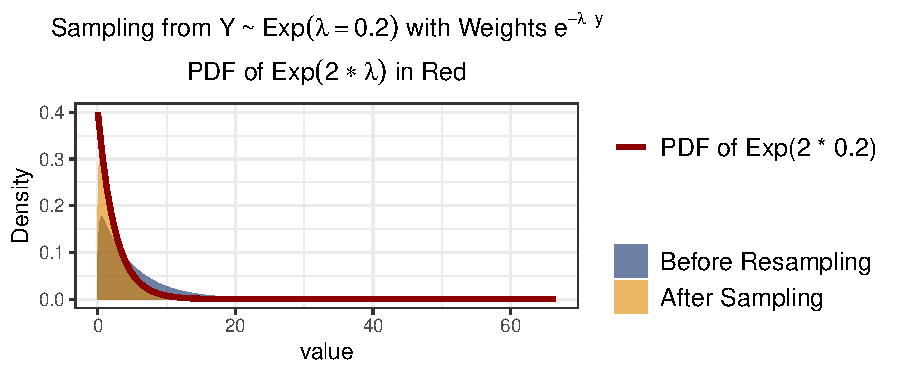
\includegraphics[width=1\linewidth]{thesis_files/figure-latex/unnamed-chunk-19-1} 

}

\caption{\label{fig:prior-induced}}\label{fig:unnamed-chunk-19}
\end{figure}
\hypertarget{pooling}{%
\subsection{Pooling}\label{pooling}}

At this point, we want to obtain the logarithmically pooled distribution of the two priors we have on \(\phi\), denoted \(f_\phi^{pooled}\).

Now, as described in greater detail in the section on the \protect\hyperlink{logpooled}{Sampling-Importance-Resampling algorithm}, the weights are \(w_i = \left( \frac{f_\phi^{direct}(M(\theta_i))}{f_\phi^{induced}(M(\theta_i))} \right)^{1-\alpha}.\)

We perform a kernel density estimation to approximate the density of \(f_\phi^{induced}(\phi)\) at the coordinates \(\phi_1, \dots, \phi_M\). To compute \(f_\phi^{direct}(\phi)\), we can use the density function \(f_\phi^{direct}\).

Once we have these weights, we resample the \(\phi_1,\dots,\phi_M\) to obtain a sample from the target distribution \(t(\alpha) \Big( f^{induced}(M(\theta)) \Big)^{0.5} \Big( f^{direct} (M(\theta)) \Big)^{0.5}\), where \(t(\alpha)\) is the normalizing constant needed to make the pooled density valid. We resample \(\theta_1, \dots, \theta_k\) with the same weights to obtain the constrained distributions for the inputs.

We see the melded distributions and pre-melding distributions in Figure \ref{fig:melded}.
\begin{figure}

{\centering 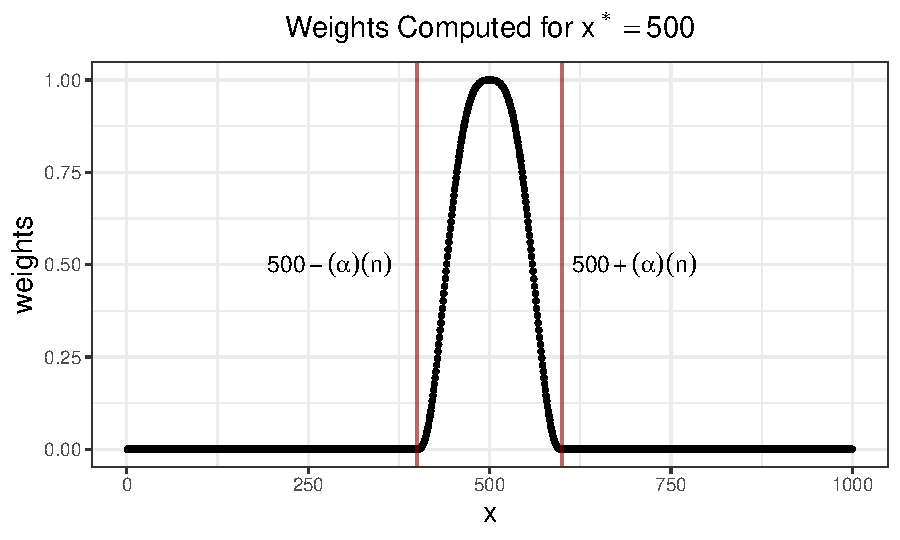
\includegraphics[width=1\linewidth]{thesis_files/figure-latex/unnamed-chunk-20-1} 

}

\caption{\label{fig:melded}}\label{fig:unnamed-chunk-20}
\end{figure}
Comparing the induced and direct priors on \(P(S_0| \text{test}_+, \text{untested})\) above, we see that although they have shared support, some values from the induced distribution we acquire by using \(M\) to generate values of \(\phi\) from sampled values of \(\theta\) are very unlikely to be in accordance with the information we know about the prevalence of SARS-CoV-2 asymptomatic infection. This is where Bayesian melding comes into play. Pooling these distributions enable us to take both the prior on \(f^{direct}\) from published analyses on asymptomatic infection, and the induced prior, \(f^{induced}\), into account to constrain the distributions of both the model inputs \(\theta = \{ \alpha, \beta, P(S_1 | \text{untested})\}\) and model output \(\phi = P(S_0|\text{test}_+, \text{untested})\) to be in accordance with both prior distributions. We then use these constrained distributions as inputs in the probabilistic bias analysis.

\hypertarget{motivating-example}{%
\subsection{Motivating Example}\label{motivating-example}}

We can see the impact of using melded priors in Suffolk county in\} Massachusetts in Figure \ref{fig:suffolkmelding}. Since using the priors without melding allows for asymptomatic rates \(P(S_0|\text{test}_+,\text{untested})\) that are extremely high, the upper bound of the estimates will be substantially higher than predicted when using the melded priors, which do not include values where the inputs lead to values of asymptomatic rate that are unsupported by available data (e.g., meta-analyses) on the asymptomatic rate.
\begin{center}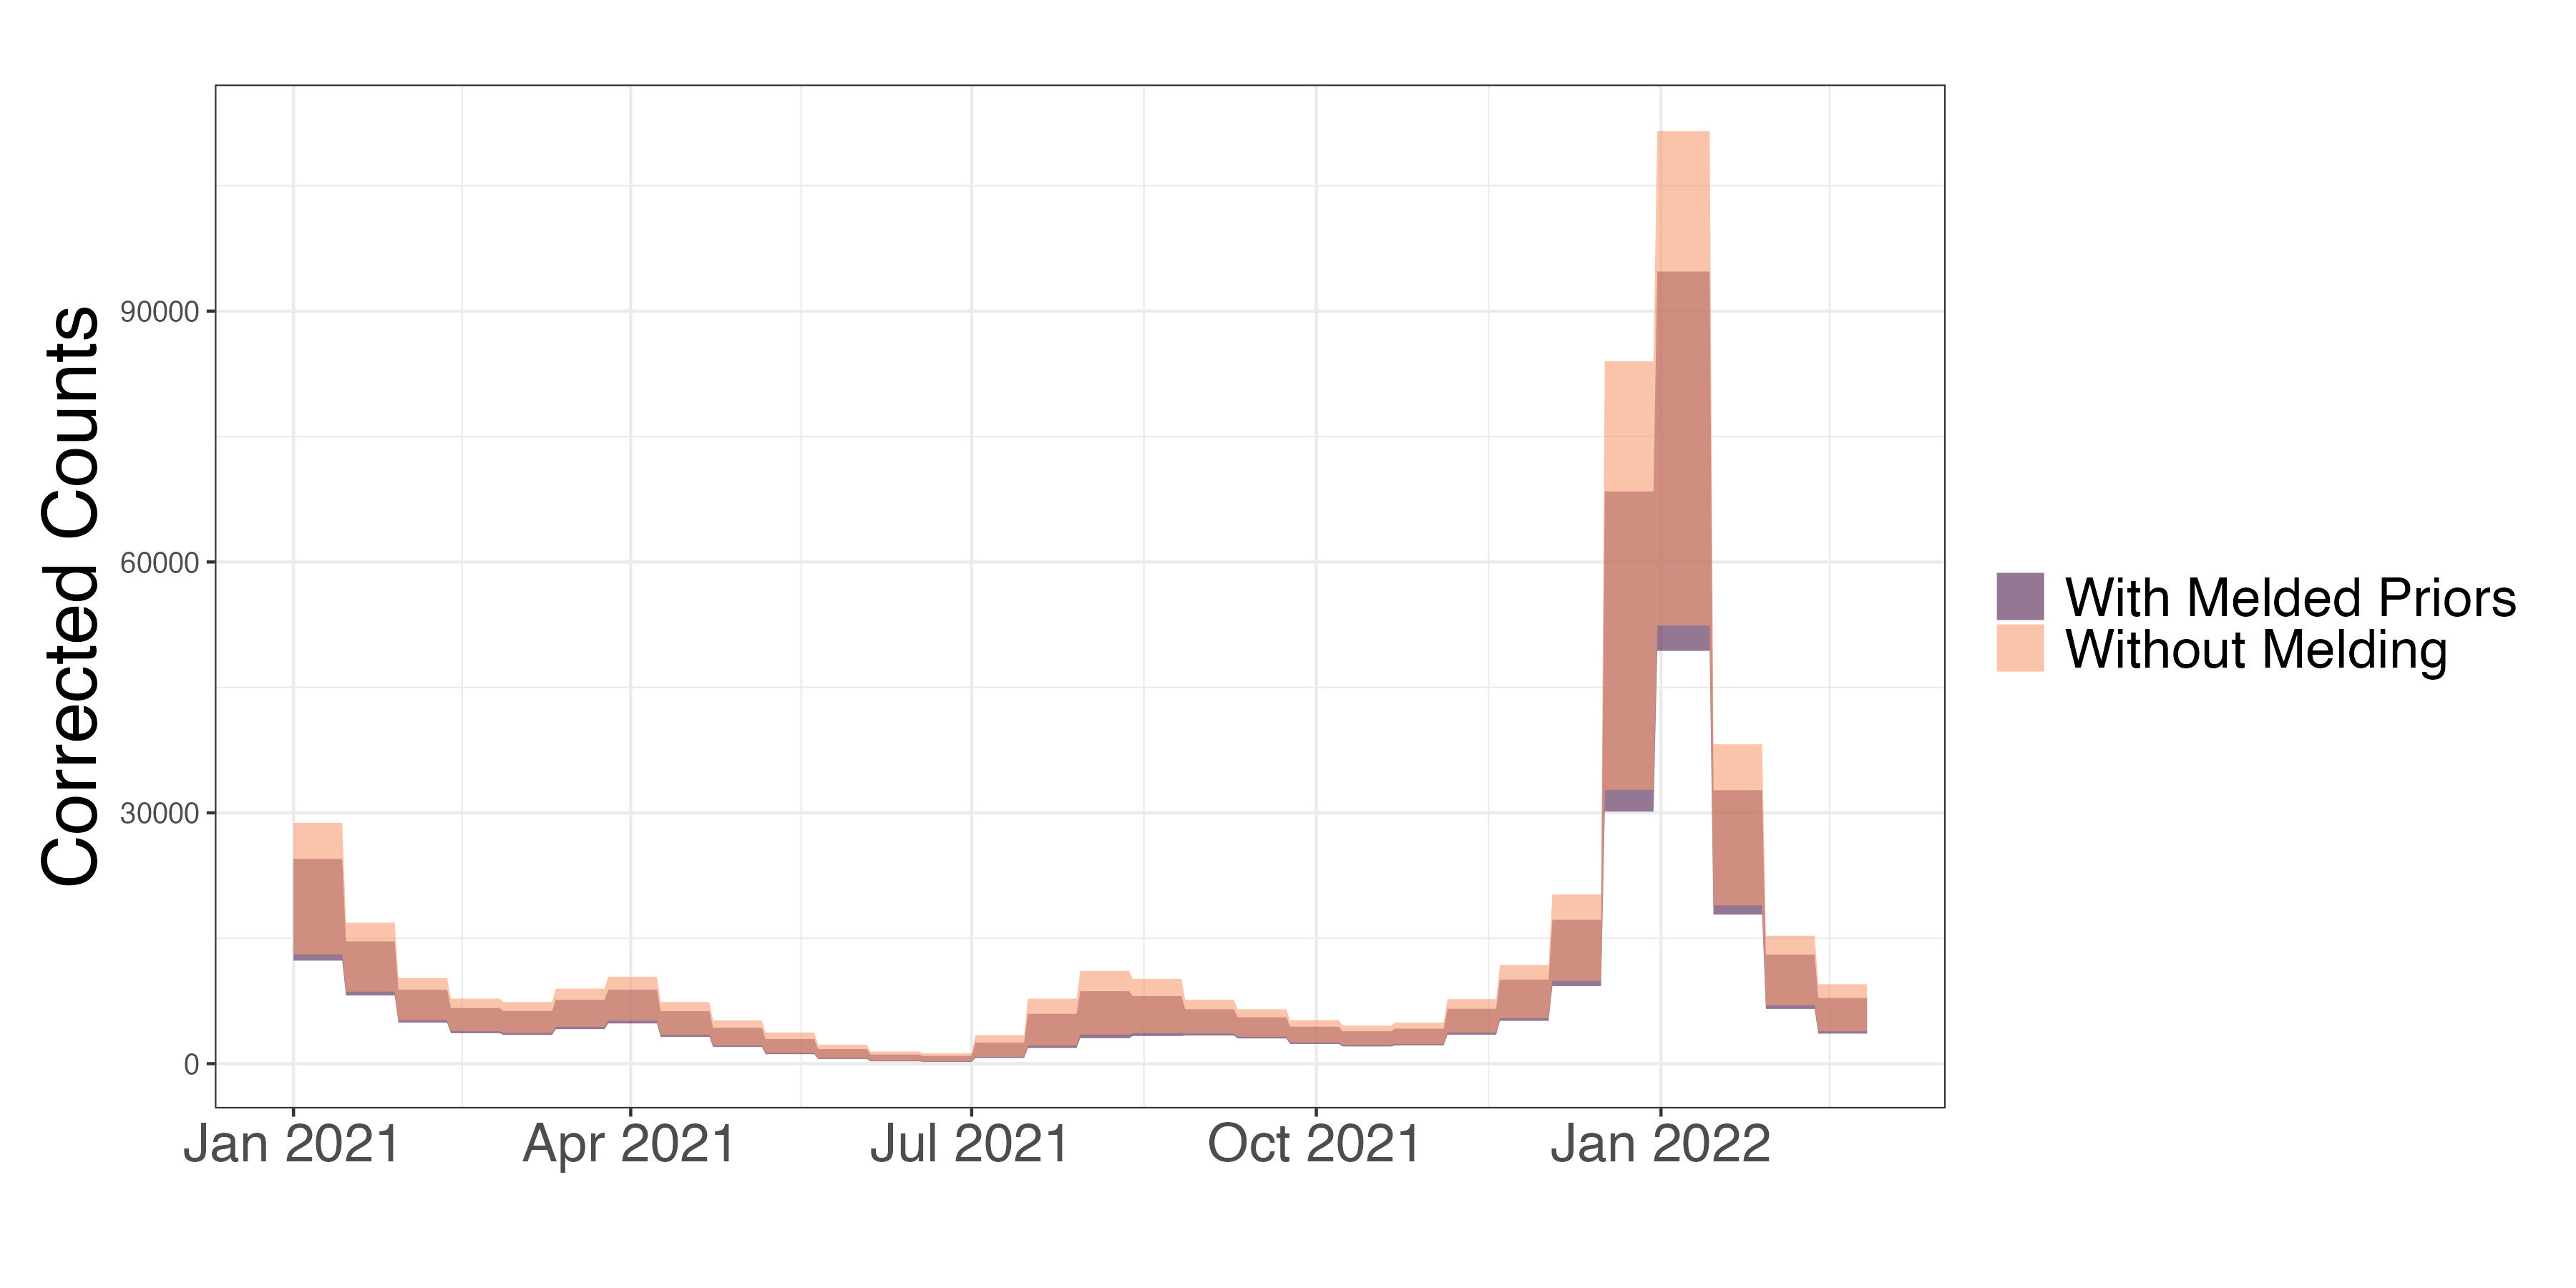
\includegraphics[width=1\linewidth]{figure/suffolk_bayesian_melding} \end{center}

\hypertarget{derivation}{%
\subsection{\texorpdfstring{Derivation of \(M\)}{Derivation of M}}\label{derivation}}

\indent We define \(\theta\) as the set of bias parameters \(\{P(S_1|\text{untested}), \alpha, \beta \}\). The parameters \(\alpha\) and \(\beta\) relate the observed overall test positivity rate to the test positivity rate we would obtain if we tested the asymptomatic and symptomatic partitions of the untested population. We define:
\begin{itemize}
\tightlist
\item
  \(\alpha = \dfrac{P(\text{test}_+|S_1,\text{untested})}{P(\text{test}_+|\text{tested})}\)
\item
  \(\beta = \dfrac{P(\text{test}_+|S_0,\text{untested})}{P(\text{test}_+|\text{tested})}\).
\end{itemize}
The parameter \(P(S_1|\text{untested})\) reflects the probability someone among the untested population has moderate to severe COVID-like symptoms.

We relate this set of parameters to the asymptomatic infection rate \(\phi = P(S_0|\text{test}_+, \text{untested})\) by the function \(M: \theta \to \phi\):
\begin{tcolorbox}
\vspace{2 mm}
\begin{align*}   
 M(\theta)  = \dfrac{\beta (1- P(S_1|\text{untested}))}{\beta(1- P(S_1|\text{untested})) + \alpha(P(S_1|\text{untested})} = P(S_0|\text{test}_+, \text{untested}).\\
\end{align*}
\end{tcolorbox}
In what follows, we show this equality holds.

\noindent Since we have \(\alpha = \frac{P(\text{test}_+|S_1, \text{untested})}{P(\text{test}_+|tested)}\) and \(\beta = \dfrac{P(\text{test}_+|S_0, \text{untested})}{P(\text{test}_+|tested)}\), we can write
\begin{align*}  &= \dfrac{\dfrac{P(\text{test}_+|S_0, \text{untested})}{P(\text{test}_+|tested)}(1 - P(S_1|\text{untested}))}{\dfrac{P(\text{test}_+|S_0, \text{untested})}{P(\text{test}_+|tested)}(1-P(S_1|\text{untested})) + \dfrac{P(\text{test}_+|S_1, \text{untested})}{P(\text{test}_+|tested)} P(S_1|\text{untested})}
\end{align*}
and cancelling out the term \(P(\text{test}_+|tested)\) we have

\[ = \dfrac{{P(\text{test}_+|S_0, \text{untested})}(1 - P(S_1|\text{untested}))}{P(\text{test}_+|S_0, \text{untested})(1-P(S_1|\text{untested})) + P(\text{test}_+|S_1, \text{untested}) P(S_1|\text{untested})}.\]

\noindent Since \(P(S_0|\text{untested}) = 1 - P(S_1|\text{untested})\),
\begin{align*} 
&=  \dfrac{{P(\text{test}_+|S_0, \text{untested})}P(S_0|\text{untested})}{P(\text{test}_+|S_0, \text{untested})P(S_0|\text{untested}) + P(\text{test}_+|S_1, \text{untested}) P(S_1|\text{untested})}.
\end{align*}
Applying the definition of conditional probability to the term
\(P(\text{test}_+|S_0, \text{untested})P(S_0|\text{untested})\) in the numerator,
\begin{align*}
&=
    \dfrac{\Big( \dfrac{P(\text{test}_+,S_0, \text{untested})}{P(S_0, \text{untested})} \Big) \Big(\dfrac{P(S_0, \text{untested})}{P(\text{untested})}\Big)}{P(\text{test}_+|S_0, \text{untested})P(S_0|\text{untested}) + P(\text{test}_+|S_1, \text{untested}) P(S_1|\text{untested})}\\ 
    &= \dfrac{\Big( \dfrac{P(\text{test}_+,S_0, \text{untested})}{P(S_0, \text{untested})} \Big) \Big(\dfrac{P(S_0, \text{untested})}{P(\text{untested})}\Big)}{P(\text{test}_+|S_0, \text{untested})P(S_0|\text{untested}) + P(\text{test}_+|S_1, \text{untested}) P(S_1|\text{untested})}\\
    &=  \dfrac{\dfrac{P(\text{test}_+,S_0, \text{untested})}{P(\text{untested})}}{P(\text{test}_+|S_0, \text{untested})P(S_0|\text{untested}) + P(\text{test}_+|S_1, \text{untested}) P(S_1|\text{untested})}\\
    &=  \dfrac{{P(\text{test}_+,S_0|\text{untested})}}{P(\text{test}_+|S_0, \text{untested})P(S_0|\text{untested}) + P(\text{test}_+|S_1, \text{untested}) P(S_1|\text{untested})}.
\end{align*}
\noindent We can substitute this result in for the \(P(\text{test}_+|S_0, \text{untested})P(S_0|\text{untested})\) term in the denominator to yield
\begin{align*}
  &=  \dfrac{{P(\text{test}_+,S_0|\text{untested})}}{P(\text{test}_+,S_0|\text{untested}) + P(\text{test}_+|S_1, \text{untested}) P(S_1|\text{untested})} \hspace{ 20 mm }
\end{align*}
With same reasoning, we can simplify
\begin{align*}
P(\text{test}_+|S_1, \text{untested})P(S_1|\text{untested}) = P(S_1, \text{test}_+|\text{untested}),
\end{align*} giving us
\begin{align*}
  &=  \dfrac{{P(\text{test}_+,S_0|\text{untested})}}{P(\text{test}_+,S_0|\text{untested}) +  P(S_1, \text{test}_+|\text{untested})} \hspace{45 mm }\\ 
   &=  \dfrac{{P(\text{test}_+,S_0|\text{untested})}}{P(\text{test}_+|\text{untested}) } \\
   &= \dfrac{\dfrac{P(S_0, \text{test}_+, \text{untested})}{P(\text{untested})}}{ \dfrac{P(\text{test}_+,\text{untested})}{P(\text{untested})}} \\ 
  &=\dfrac{P(S_0, \text{test}_+, \text{untested})}{P(\text{test}_+,\text{untested})} \\
  &= P(S_0 |\text{test}_+, \text{untested}).
\end{align*}
\noindent Hence, we have
\begin{align*}
P(S_0 |\text{test}_+, \text{untested}) = \dfrac{\beta (1- P(S_1|\text{untested}))}{\beta(1- P(S_1|\text{untested})) + \alpha(P(S_1|\text{untested})}
\end{align*}
\noindent as desired.
\qed

\newpage

\hypertarget{sampling}{%
\section{Sampling-Importance-Resampling Algorithm}\label{sampling}}

\hypertarget{overview}{%
\subsection{Overview}\label{overview}}

~~~The Sampling-Importance-Resampling Algorithm, introduced in Rubin (1987), is a non-iterative method for approximating a sample from a target probability density function \(f\). This algorithm is fundamental to the implementation of Bayesian melding.

The two main steps are the sampling step and importance resampling step. We have two (generally distinct) sample sizes, where \(m\) is the initial sample size and \(r\) is the resample size.

In the sampling step, we draw an independent and identically distributed sample of size \(m\) from \(g\), \(Y_1, Y_2, \dots, Y_m\). Then, we compute weights \(h(Y)\) such that \(g \cdot h \propto f\). That is, we set the weights

\[w_i = h(Y_i) = \dfrac{\frac{f(Y_i) } {g(Y_i)} }{\sum_{i=1}^m\frac{f(Y_i) } {g(Y_i)} }.\]

We resample with these defined weights to obtain a sample of size \(r\) from \(Y_1, Y_2, \dots, Y_m\). We denote this resample \(Z_1,\dots, Z_r\). With these weights, \(Z_1,\dots, Z_r\) is approximately a sample from \(f\).

The method is most efficient when \(g\) is a good approximation of \(f\). The relationship between the sample size \(m\) and resample size \(r\) also has implications for the quality of the approximation. The algorithm generates independent and identically distributed samples as \(m/r \to \infty\), but in most applications \(m/r\) between 10 and 20 is appropriate (Rubin, Gelman, \& Meng, 2004). The practical implications of this choice are discussed \protect\hyperlink{presamp}{later in this section}.

To better understand the use of this algorithm, we provide a proof that formally relates the choice of \(g\), weights \(h\), and the target distribution \(f\). We then follow up with a couple concrete examples where there is a closed formed solution to visualize how the algorithm works in practice.

\hypertarget{proof}{%
\subsection{Proof that Algorithm Obtains Approximate Sample from Target Distribution}\label{proof}}

To gain further insight into how sampling with weights
\(w_i = \left( \frac{f_\phi^{direct}(M(\theta_i))}{f_\phi^{induced}(M(\theta_i))} \right)^{0.5}\)
approximates a sample from the target distribution the logarithmically pooled distribution \(f^{pooled}\), we first prove a more general result.
\begin{tcolorbox}[title=Function $M$ Relating Testing Positivity Parameters to Asymptomatic Rate]
Suppose we sample $Y_1, Y_2, \dots, Y_m$ independently and identically distributed with probability density function  $g$ and compute the weights
\[ w_i =\dfrac{h(Y_i)}{\sum_{i=1}^mh(Y_i) }\]
for some nonnegative function $h$ defined on the support of $Y$.

If  we sample $Z_1, \dots, Z_r$ from the discrete distribution $Y_1,\dots, Y_m$ such that 

\[ P(Z = Y_i) = \dfrac{h(Y_i)}{\sum_{i=1}^mh(Y_i) } = w_i ,\]
then $Z_1, \dots, Z_r$ is approximately a sample with density proportional to $h \cdot g$.

\end{tcolorbox}
\vspace{5 mm}

Since \(Z\) is sampled from \(Y\), we have
\[ P(Z \leq x ) = \sum_{z_i \leq x} P(Z=z_i) = \sum_{Y_i \leq x} P(Z=Y_i) .\]

We can take this sum to be over all possible values of \(Y\) by including the indicator function \(\mathbb{I} (Y_i \leq x)\), yielding
\[  = \sum_{i = 1}^m P(Z=y_i)\;\;\mathbb{I} (Y_i \leq x).  \]
and since \(P(Z=Y_i) = \dfrac{h(Y_i)}{\sum_{i=1}^mh(Y_i) }\) by definition we have
\begin{align*} 
&= \sum_{i = 1}^m \dfrac{h(Y_i)}{\sum_{i=1}^mh(Y_i) }  \;\;\mathbb{I} (Y_i \leq x)   \\
&=  \left( \dfrac{1}{ {\sum_{i=1}^mh(Y_i) }} \right) {\sum_{i=1}^mh(Y_i) }  \;\;\mathbb{I} (Y_i \leq x)   \\
&=   \dfrac{ {\sum_{i=1}^mh(Y_i) }  \;\;\mathbb{I} (Y_i \leq x) }{\sum_{i=1}^mh(Y_i) } \\
&=   \dfrac{ \frac 1m {\sum_{i=1}^mh(Y_i) }  \;\;\mathbb{I} (Y_i \leq x) }{\frac 1m \sum_{i=1}^mh(Y_i) }. \\
\end{align*}
Now, we need the Weak Law of Large Numbers. That is, if we have a sequence of random variables \(X_1, X_2, \dots\) with finite variance, then,
\[ \lim_{n \to \infty} \left( \frac{1}{n} \sum_{i=1}^n X_i \right)  = E(X_i). \]

Applying this law to both the numerator and denominator, we obtain
\begin{align*}  \lim_{m \to \infty} \left( \dfrac{ \frac 1m {\sum_{i=1}^mh(Y_i) }  \;\;\mathbb{I} (Y_i \leq x) }{\frac 1m \sum_{i=1}^mh(Y_i) } \right) &= \dfrac{ E_g[ h(Y) \;\; \mathbb I (Y \leq x) ]  }{ E_g[ h(Y) ]  }\\
&= \dfrac{\int_{-\infty}^\infty h(y) \;\; \mathbb I (y \leq x) \; g(y) \; dy}{\int_{-\infty}^\infty h(y) \, g(y) \;dy}\\
&= \dfrac{\int_{-\infty}^x h(y) \, g(y) dy}{\int_{-\infty}^\infty h(y) \, g(y) \;dy}\\
&\propto \int_{-\infty}^x h(y) \, g(y) dy. 
\end{align*}
It follows that the probability density function of \(Z\) is proportional to \(h \cdot g\).

\vspace{3 mm}

\qed

It is easiest to understand the Sampling-Importance-Resampling Algorithm when the resampled distribution has a closed form, which we can see in the following two examples.

\newpage

\hypertarget{example-1}{%
\subsubsection{Example 1:}\label{example-1}}

Suppose \(Y \sim Exp(\lambda)\), so we have the PDF \(f_Y(y) = \lambda e^{-\lambda y}\), and we sample \(Z_1,\dots,Z_r\) from \(Y_1, \dots, Y_m\) with weights direction proportional to \(X\), that is, \(h(Y) = Y\).

Then \(Z_1,\dots Z_r\) is approximately a sample from \(h(x) \; f_Y(y) = y \; \lambda e^{-\lambda y}\).

From the PDF of the gamma distribution, \(\dfrac{\beta^\alpha}{\Gamma(\alpha) }y^{\alpha - 1} e^{-\beta y}\) we can recognize that \(y \cdot e^{-\lambda y}\) corresponds to the gamma distribution with \(\alpha = 2\) and \(\beta = \lambda\).

We can see this result by considering \(Y\) before and after resampling below (Figure \ref{fig:ex1}).
\begin{figure}

{\centering 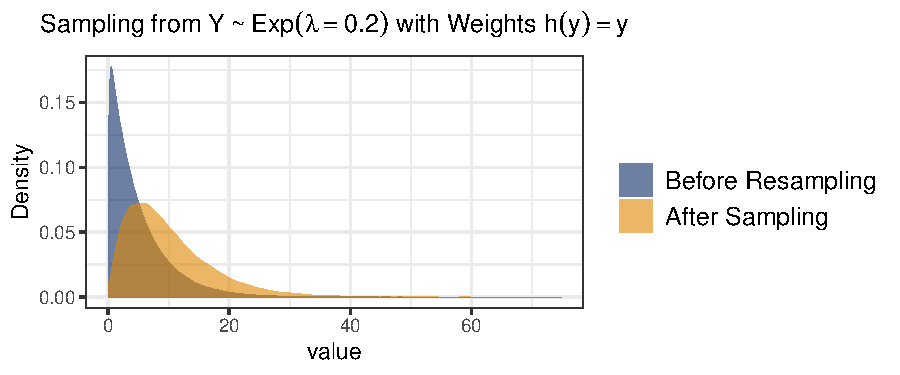
\includegraphics[width=1\linewidth]{thesis_files/figure-latex/unnamed-chunk-23-1} 

}

\caption{\label{fig:ex1}}\label{fig:unnamed-chunk-23}
\end{figure}
Then, we can see that the PDF of the the gamma distribution with \(\alpha = 2\) and \(\beta = \lambda\) corresponds to the post-sampling distribution as expected (Figure \ref{fig:ex12}).
\begin{figure}

{\centering 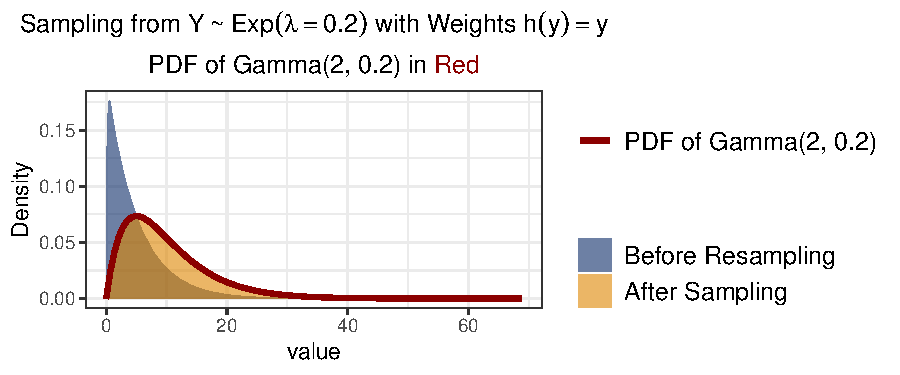
\includegraphics[width=1\linewidth]{thesis_files/figure-latex/unnamed-chunk-24-1} 

}

\caption{\label{fig:ex12}}\label{fig:unnamed-chunk-24}
\end{figure}
\newpage

\hypertarget{example-2}{%
\subsubsection{Example 2:}\label{example-2}}

Similarly, again suppose \(Y \sim Exp(\lambda)\), so \(f_Y(y) = \lambda e^{-\lambda y}\). However, now we sample with weights defined by \(h(y)= e^{-\lambda y}\).
Then our sample \(Z_1,\dots,Z_r\) is approximately a sample from
\begin{align*} 
h(y) \; f_Y(y) &=   e^{-\lambda y} \cdot \lambda e^{-\lambda y}\\
&= \ e^{-2 \lambda y}  
\end{align*}
which is proportional to the exponential distribution with parameter \(2\lambda\).

The distributions before and after resampling are shown in Figure \ref{fig:ex2}.
\begin{figure}

{\centering 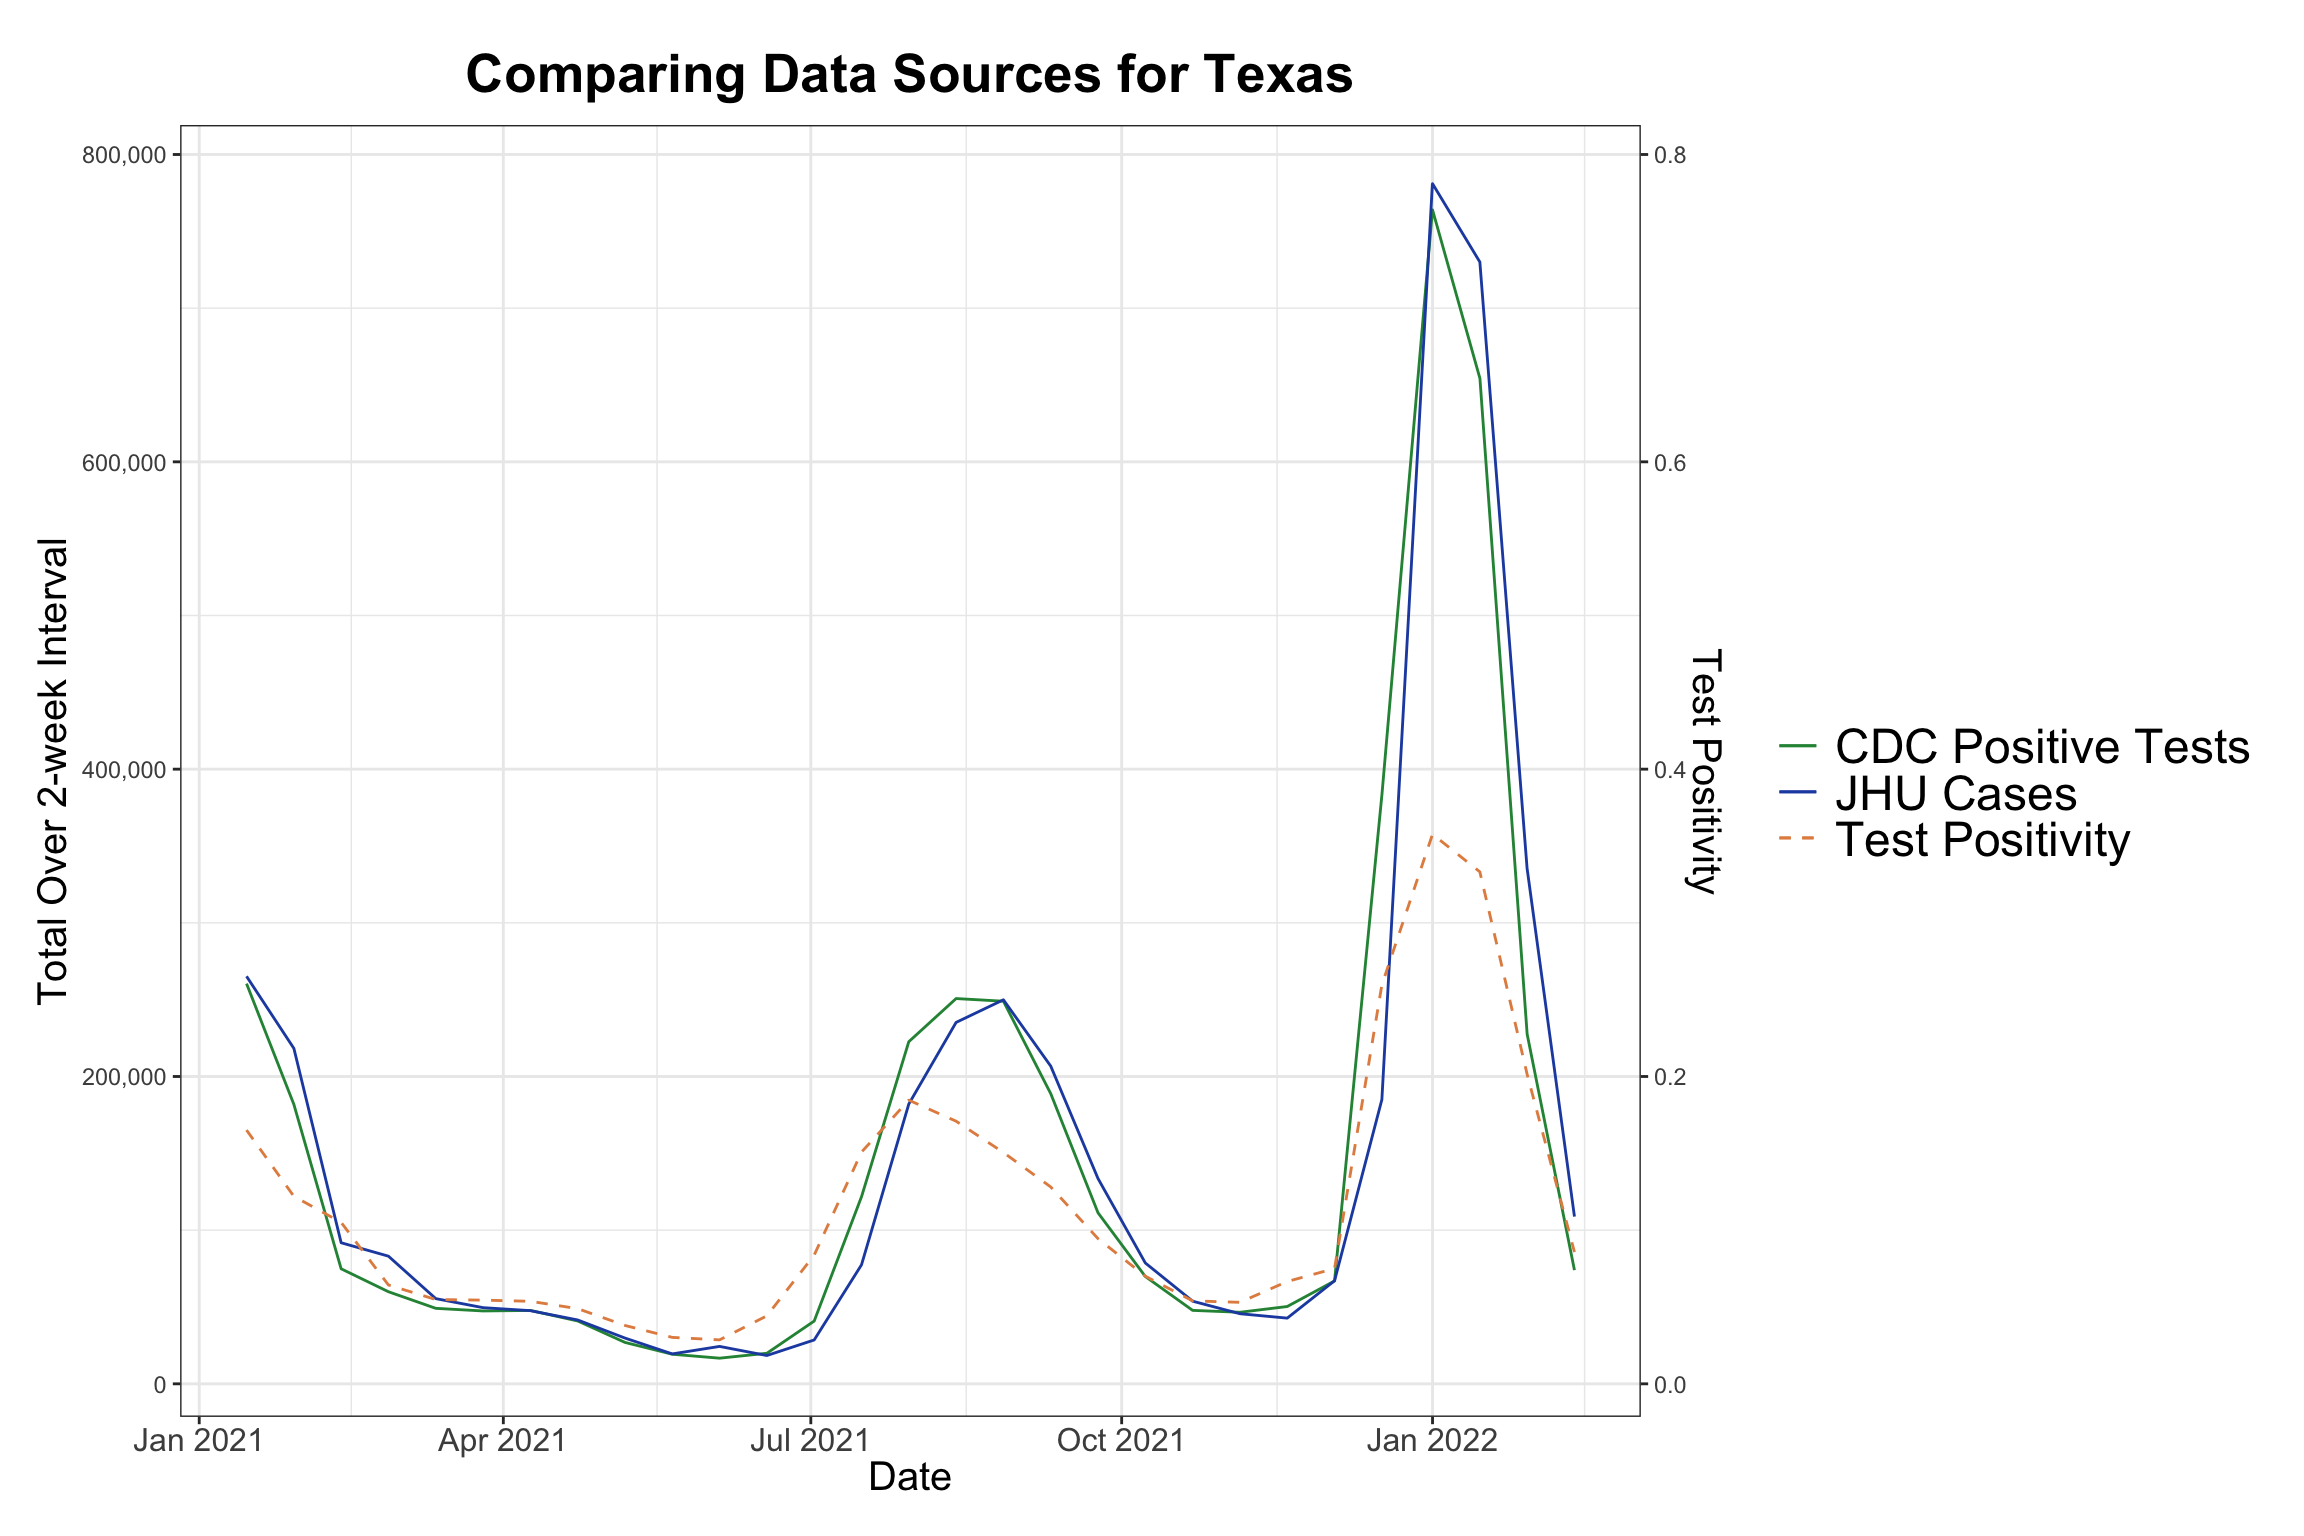
\includegraphics[width=1\linewidth]{thesis_files/figure-latex/unnamed-chunk-25-1} 

}

\caption{\label{fig:ex2}}\label{fig:unnamed-chunk-25}
\end{figure}
and then plotting the PDF of the exponential distribution with parameter \(2\lambda\) we can see the correspondence to the post-sampling distribution (Figure \ref{fig:ex22}).
\begin{figure}

{\centering 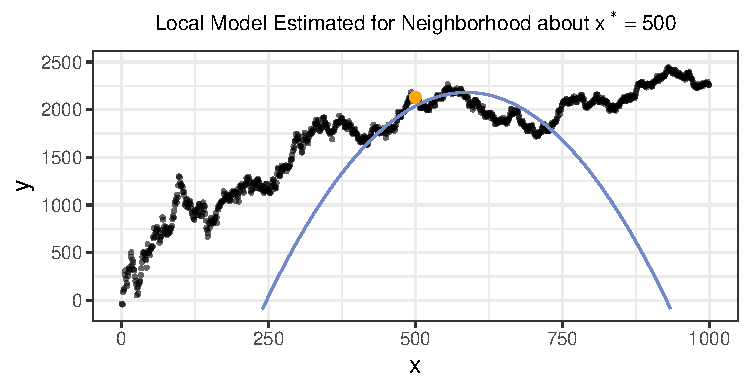
\includegraphics[width=1\linewidth]{thesis_files/figure-latex/unnamed-chunk-26-1} 

}

\caption{\label{fig:ex22}}\label{fig:unnamed-chunk-26}
\end{figure}
\newpage

\hypertarget{logpooled}{%
\subsection{Obtaining Logarithmic Pooled Distribution with the Sampling-Importance-Resampling Algorithm}\label{logpooled}}

As outlined in Carvalho, Villela, Coelho, \& Bastos (2023), we can formally define logarithmic pooling as follows.

If we have a set of densities \(\{ f_1(\phi), f_2(\phi), \ldots, f_n(\phi)\}\) and corresponding pooling weights \(\boldsymbol{\alpha}=\{\alpha_1, \alpha_2, \ldots, \alpha_n\}\), then the pooled density is
\[f^{\text{pooled}}(\phi) = t(\boldsymbol{\alpha}) \prod_{i=0}^n f_i(\phi)^{\alpha_i},\]
where \(t(\boldsymbol{\alpha})\) is the normalizing constant \(t(\boldsymbol{\alpha}) = \dfrac{1}{ \int_{\Phi}\prod_{i=0}^n f_i(\phi)^{\alpha_i} d\phi}\) to ensure the pooled density is a valid probability density.

The case for this work is more simple: we only have two densities we wish to pool, \(f_\phi^{induced}\) and \(f_\phi^{direct}\), and we assign them equal weights by letting \(\boldsymbol{\alpha} = \{.5, .5\}\). This yields

\[f^{pooled}(\phi) = t(\boldsymbol \alpha) \left( f^{induced} (\phi) \right)^{0.5} \left( f^{direct} (\phi) \right)^{0.5}.\]

Since our target distribution is \(t(\boldsymbol \alpha) \left( f^{induced} (\phi) \right)^{0.5} \left( f^{direct} (\phi) \right)^{0.5}\), and we have a sample from \(f^{induced}\), we compute the weights such that
\begin{align*} w_i &\propto \dfrac{ \left( f^{induced} (\phi_i) \right)^{0.5} \left( f^{direct} (\phi_i) \right)^{0.5} } {f^{induced}(\phi_i)} \\
&=  \dfrac{ \left( f^{direct} (\phi_i) \right)^{0.5} } {\left( f^{induced} (\phi_i) \right)^{0.5} } \\
&=   \left( \dfrac{  f^{direct} (\phi_i) } { f^{induced} (\phi_i) }  \right)^{0.5}. \\
\end{align*}
Sampling from \(f^{induced}\) with these weights will yield a sample with approximately the target density \(t(\alpha) \left(f^{induced} (\phi) \right)^{0.5} \left( f^{direct} (\phi)\right)^{0.5}\) from the result in the \protect\hyperlink{proof}{previous section}.

\hypertarget{presamp}{%
\subsection{Implications of the Sample Size and Resample Size}\label{presamp}}

When we have an initial sample of size \(m\) from \(g\), denoted \(Y_1,\dots,Y_m\), and take a weighted sample of size \(r\), \(Z_1,\dots,Z_r\), the choices of \(m\) and \(r\) can have notable effects on the estimated distribution of the resample. In particular, when the sample size and resample size do not differ substantially, it becomes more likely that we will sample some element of \(Y_1,\dots,Y_m\) more than once. This can result in irregularities in the estimated distribution of \(Z_1,\dots,Z_r\). We see this in \ref{fig:prepostsamp} when the ratio of \(m/r\) is closer to 1, while the problem reduces as we increase the sample size \(m\) compared to the posterior (resample) size \(r\).
\begin{figure}

{\centering 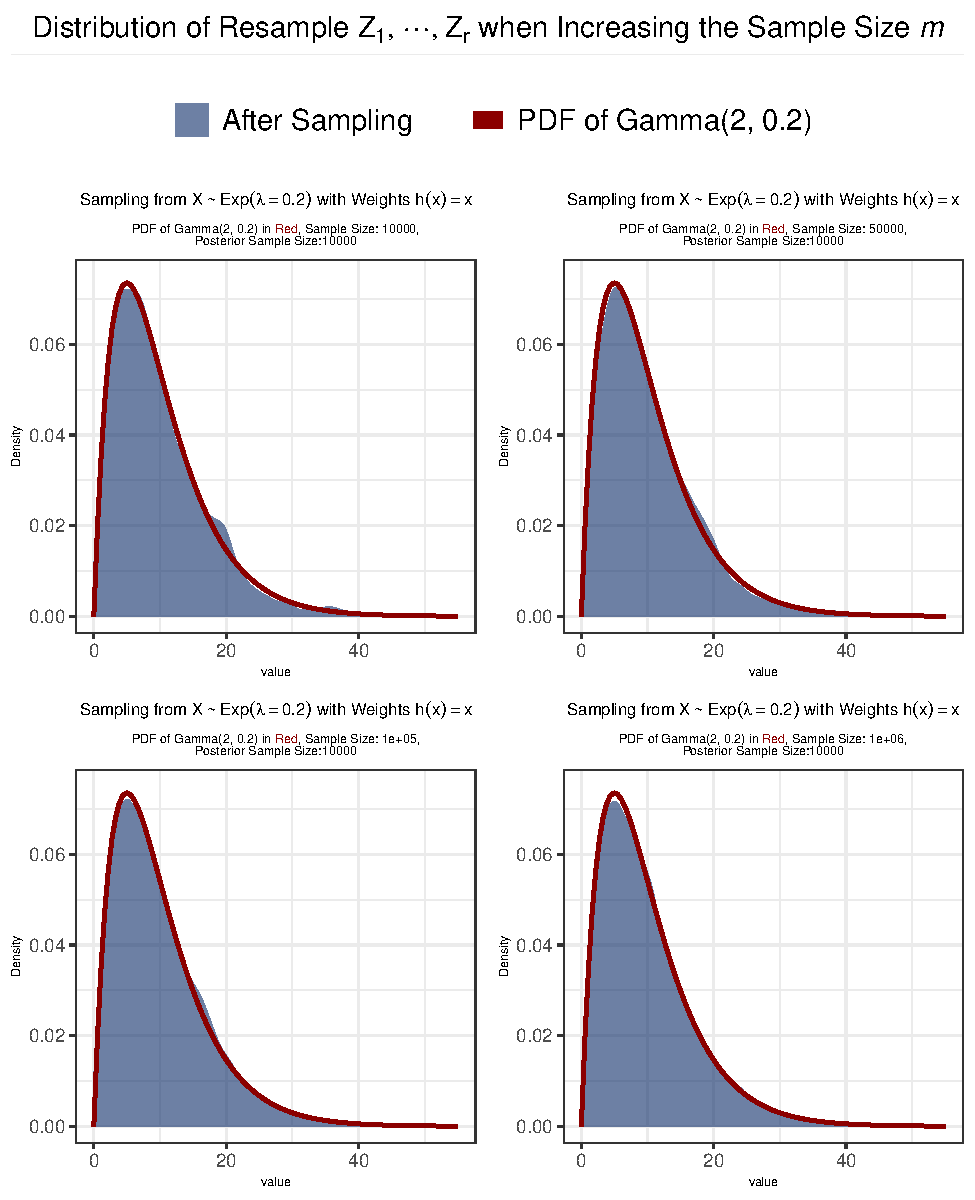
\includegraphics[width=1\linewidth]{thesis_files/figure-latex/pre-post-sampling-code-1} 

}

\caption{\label{fig:prepostsamp}}\label{fig:pre-post-sampling-code}
\end{figure}
When using the Sampling-Importance-Resampling algorithm to obtain the logarithmically pooled distribution, see the effect of this choice has a major impact when we are melding truncated distributions. The pooled distribution is only defined on the intersection of the supports of the distributions being pooled. Truncation, then, can limit the choices of \(Y_1,\dots, Y_m\) we take when resampling, which can lead to substantial irregularities in the resulting estimated pooled distribution (Figure \ref{fig:trunc}).
\begin{figure}

{\centering 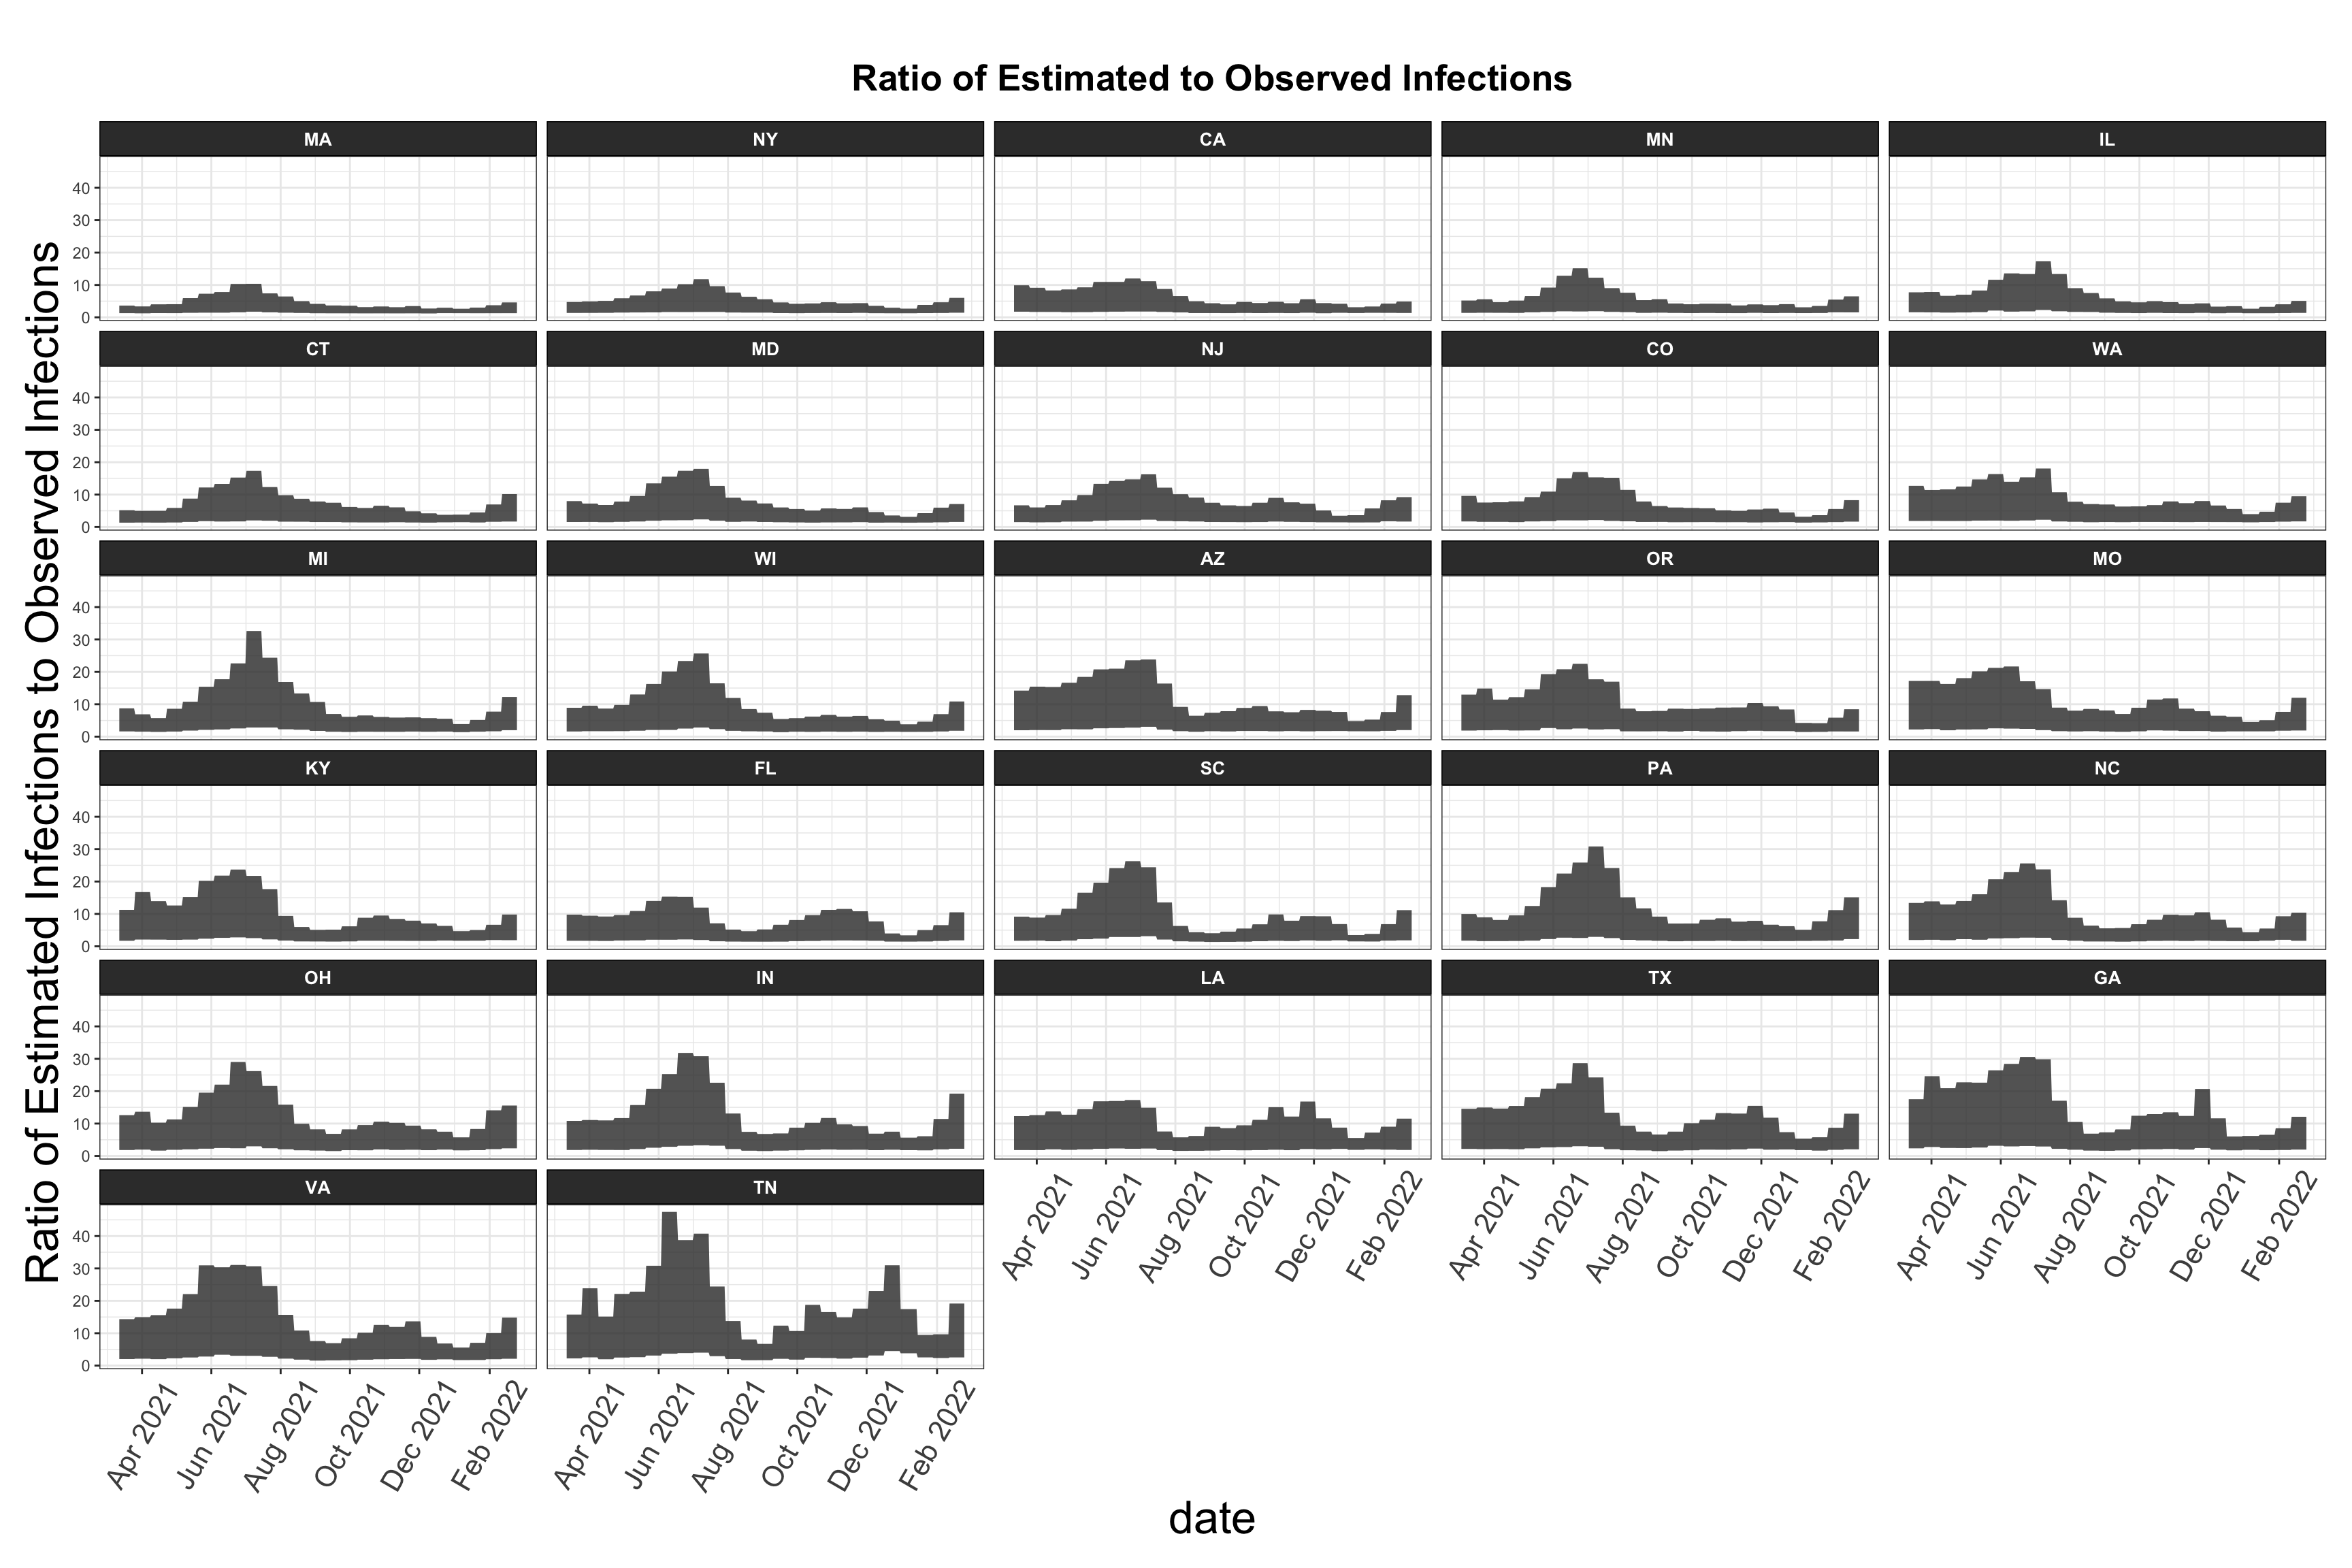
\includegraphics[width=1\linewidth]{thesis_files/figure-latex/unnamed-chunk-29-1} 

}

\caption{\label{fig:trunc}}\label{fig:unnamed-chunk-29}
\end{figure}
\newpage

\hypertarget{loess-smoothing}{%
\section{LOESS Smoothing}\label{loess-smoothing}}

\hypertarget{introduction-1}{%
\subsection{Introduction}\label{introduction-1}}

Locally estimated scatterplot smoothing (LOESS) fits a collection of local regression models to obtain a smooth curve through the observed data (Figure \ref{fig:loess}). It is highly flexible in the sense that we do not have to specify the functional relationship between the predictor and response variable for the entire range of the predictor, which may be impossible in various settings. It is particularly useful when working with time series data with substantial noise.
\begin{figure}

{\centering 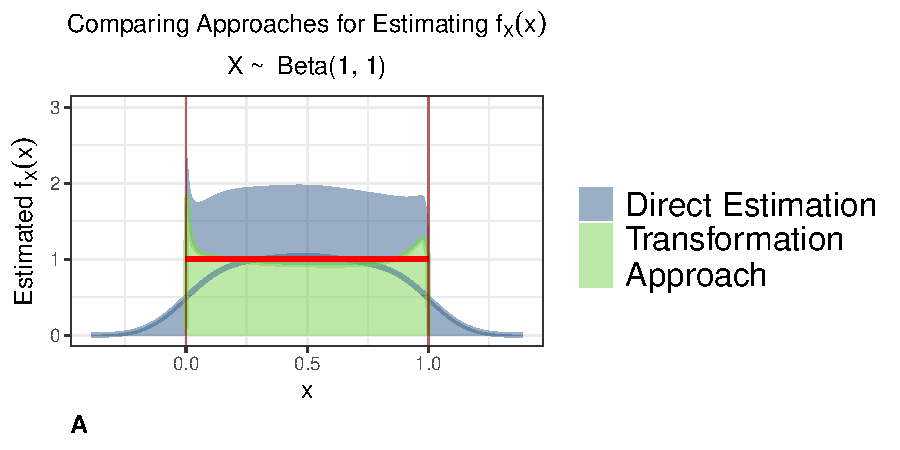
\includegraphics[width=1\linewidth]{thesis_files/figure-latex/unnamed-chunk-31-1} 

}

\caption{\label{fig:loess}LOESS curve fitted with  a span of 0.2. }\label{fig:unnamed-chunk-31}
\end{figure}
To perform LOESS smoothing, we estimate a set of local regressions (Chambers, 1997). To do this, we must specify the span; this smoothing parameter is the fraction of the data that is used for the local polynomial fit. With a smaller span, the resulting curve will fit the trends more closely, while a larger span reflects broader trends (Figure \ref{fig:smooth-spans}).
\begin{figure}

{\centering 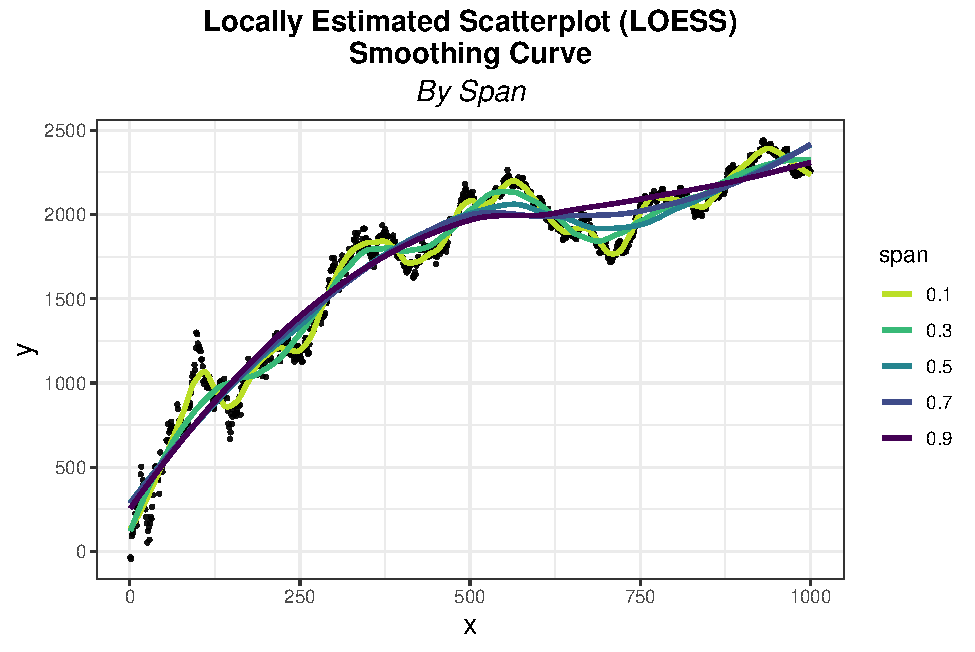
\includegraphics[width=1\linewidth]{thesis_files/figure-latex/unnamed-chunk-32-1} 

}

\caption{\label{fig:smooth-spans}}\label{fig:unnamed-chunk-32}
\end{figure}
\hypertarget{fitting-the-loess-curve}{%
\subsection{Fitting the LOESS Curve}\label{fitting-the-loess-curve}}

To introduce some notation for the model at hand, we have a dependent variable \(\mathbf y\) and independent variable \(\mathbf x\), where \(\mathbf y\) and \(\mathbf x\) are related by some unknown function \(g\), that is, \(y = g(x) + \boldsymbol \epsilon\)\footnote{Recall we use bold type for vectors, e.g., \(\mathbf x \in \mathbb R^n\) is a vector with observations \(x_i \in \mathbb R\).}. When we want to use LOESS smoothing to estimate \(g\), often this function is complex, so we break up the problem into estimating a set of local regressions.

To obtain a predicted value \(\hat g(x^*)\) for a particular value of the independent variable \(x^*\), we fit a polynomial with greatest weight placed on points in the neighborhood of \(x^*\), where the width of this neighborhood is defined by the choice of smoothing span. Let \(\alpha \in (0,1]\) denote the chosen smoothing span.

For a particular value of \(x^*\), we estimate the predicted value \(\hat g(x^*)\) by fitting a local regression. We first compute the weights by computing the vector of distances from this point \(x^*\), that is,

\[\Delta (x^*) = |\mathbf x -x^* | \]

We define \(q = \text{floor}(\alpha n)\), and take \(\Delta_q(x^*) \in \mathbb R\) to be the \(q^th\) smallest distance of \(\Delta (x^*)\).

The vector of weights is then
\[T(\Delta(x^*), \Delta_q(x^*))\]

where \(T\) is the tricube weight function given by

\[
T(x) = \begin{cases} (1-(x)^3)^3 \hspace{9 mm}  \text{ for } |x| < 1\\
0  \hspace{25 mm} \text{ for |x| } \geq 1 \end{cases}.
\]
Essentially, this process gives weight to points in the neighborhood of \(x^*\). Consider \(x^* = 500\) and \(\text{smoothing span} = \alpha = .2\).

Then the weights we obtain are given in Figure \ref{fig:weights}.
\begin{figure}

{\centering 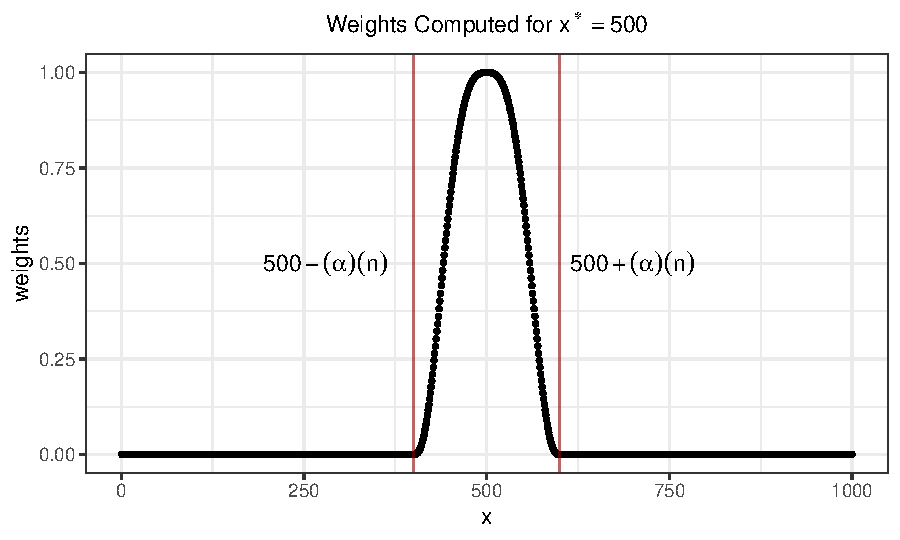
\includegraphics[width=1\linewidth]{thesis_files/figure-latex/unnamed-chunk-33-1} 

}

\caption{\label{fig:weights} The only values with nonzero weights are those within the interval $(500 - \alpha (n), 500 - \alpha (n))$. That is, the proportion $\alpha$ of the data points closest to $x^*$ will have nonzero weights.}\label{fig:unnamed-chunk-33}
\end{figure}
\newpage

We fit a linear regression with polynomial terms, typically with degree up to 2, with these weights. For example, fitting the model for this same \(x^*=500\), we obtain the polynomial in Figure \ref{fig:ex-poly}.
\begin{flushleft}
\begin{figure}

{\centering 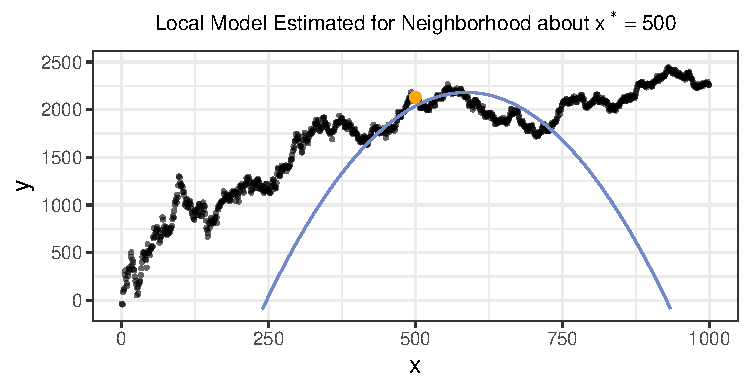
\includegraphics[width=1\linewidth]{thesis_files/figure-latex/unnamed-chunk-34-1} 

}

\caption{\label{fig:ex-poly}}\label{fig:unnamed-chunk-34}
\end{figure}
\end{flushleft}
By fitting the model for every point in \(\mathbf x\), we obtain the smoothed line shown in red in Figure \ref{fig:loess-all}.
\begin{figure}

{\centering 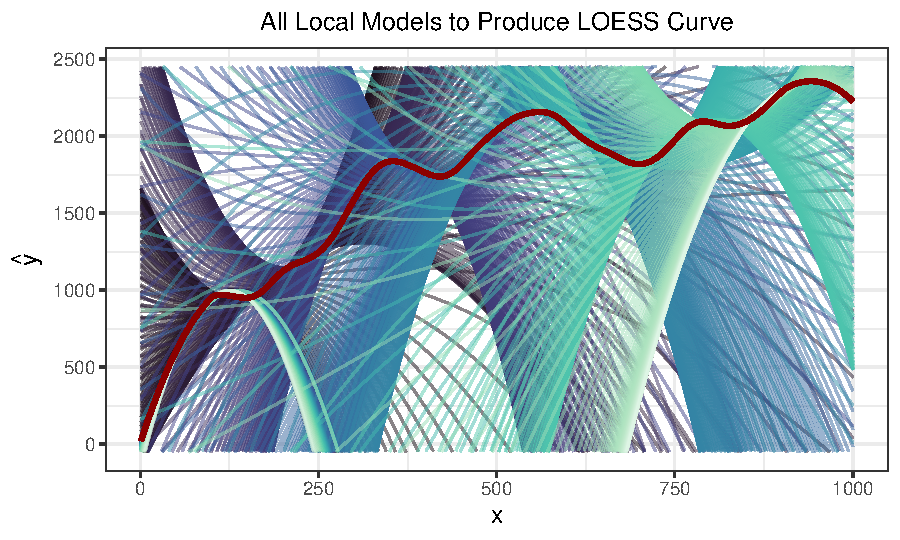
\includegraphics[width=1\linewidth]{thesis_files/figure-latex/loess-all-1} 

}

\caption{\label{loess-all}}\label{fig:loess-all}
\end{figure}
Smoothing methods are sensitive to the choice of smoothing parameter \(h\), which represents the fraction of the data that is used for the local polynomial fit.

Methods exist for picking the smoothing parameter \(h\) that minimizes the mean squared error between the predicted values from the estimated line and observed values of the dependent variable, for example, leave-one-out cross-validation or generalized cross-validation.

However, for this work, we used LOESS smoothing to smooth survey data from the COVID-19 Trends and Impact Survey (Reinhart et al., 2021).
We choose the smoothing parameter for each variable based on domain knowledge regarding the level of noise present for each variable of interest. For example, there is substantial noise in the screening test positivity data that reflect trends that do not represent meaningful differences in the screening test positivity. Some trends in the screening sensitivity may be due to scheduled workplace screenings happening at regular time intervals, and some of the variation may be due to the frequency of screening testing due to other variables, such as the access and cost of testing.

Since the ratio \(\frac{\text{screening test positivity}}{\text{overall test positivity}}\) is used to estimate \(\beta = \frac{P(\text{test}_+| S_0, \text{untested})}{P(\text{test}_+|tested)}\), the variability in the screening positivity creates substantial variability in our estimates of \(\beta\).

In light of this variability and the presence of other trends regarding the screening test positivity, we set the span to \(\frac{4}{12} = 0.33\) to fit the local regressions for 4-month intervals with the aim to capture the broader trends over time.

There was less variabiity in the smoothing span for the weighted percentage of COVID-like Illness, the estimate of \(P(S_1|\text{untested})\). Hence, we set the smoothing parameter to \(0.2\) detect trends at a finer time scale.

Sensitivity analyses with modified versions of the smoothing span of \(\beta\) are included in the appendix in the section INCLUDE SECTION.

\newpage

\hypertarget{kernel-density-estimation}{%
\section{Kernel Density Estimation}\label{kernel-density-estimation}}

\hypertarget{overview-1}{%
\subsection{Overview}\label{overview-1}}

When we have a random sample \(X_1,\dots X_n\) drawn from the density \(f_X\) and we want to estimate \(f_X\) at some set of points, we can use kernel density estimation. This is relevant in this work for estimating \(f^{induced}\).

We define a kernel function as follows (Wasserman, 2006).
\begin{tcolorbox}[title=Definition: Kernel Function]

A kernel function $K$ is a smooth nonnegative function such that 

$$\int K(x) \; dx = 1, \int x K(x) dx = 0, \sigma^2_k \equiv \int x^2 K(x) dx > 0.$$ 
\end{tcolorbox}
The Gaussian kernel \(K(x) = \frac{1}{\sqrt{2\pi}}e^{-x^2/2}\) is commonly used in practice; the tricube kernel, as discussed in the LOESS smoothing section, is another valid kernel function.

The kernel density estimator is

\[\hat f_n(x) = \frac 1n \sum_{i=1}^n \frac 1h K\left(\dfrac{x-X_i}{h} \right)\]

where \(h\) is the smoothing parameter or bandwidth. In Figure \ref{fig:kernel}, we see the effect of increasing the bandwidth \(h\): larger values result in smoother curves, while smaller values result in curves that follow the histogram more closely.
\begin{figure}

{\centering 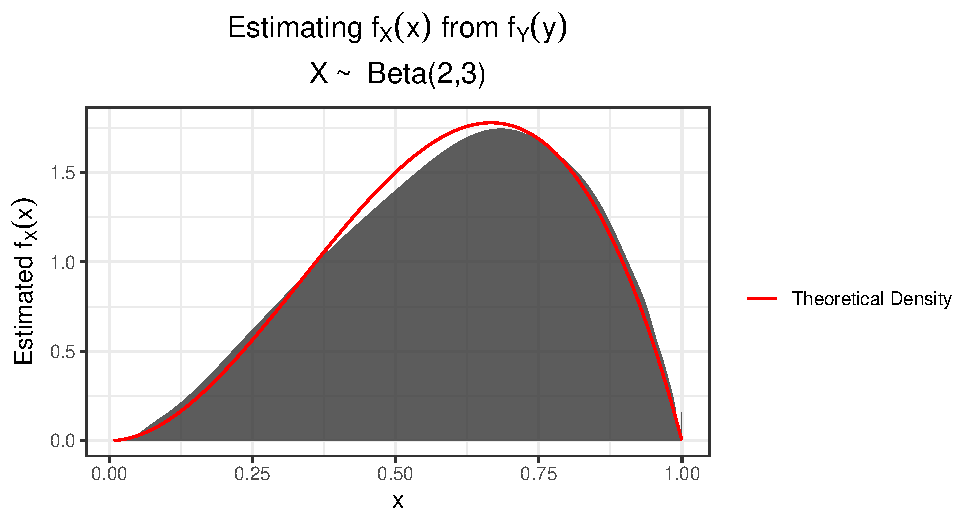
\includegraphics[width=1\linewidth]{thesis_files/figure-latex/unnamed-chunk-38-1} 

}

\caption{\label{fig:kernel}}\label{fig:unnamed-chunk-38}
\end{figure}
\hypertarget{bounded-density-estimation}{%
\subsection{Bounded Density Estimation}\label{bounded-density-estimation}}

A question warranting investigation is the choice of kernel given we are working with a bounded variable -- the density we seek to estimate, \(f^{induced}\) is the density of \(P(S_0|\text{untested}, \text{test}_+)\) and hence is bounded between 0 and 1.

One way to handle density estimation for a bounded variable \(X\) is by performing a transformation
\(X=g(Y)\) and then using the change of variables for a probability density to obtain \(f_X(x)\) (Aurelien Pelissier, 2022).

Since \(X \in [0,1]\) and we want to transform it to the range \((-\infty,\infty)\), we can let \(Y = \text{logit}(X) = \log \left( \frac{X}{1-X} \right)\).

We know if we have \(X = g(Y)\), then we can acquire the distribution of \(X\) from that of \(Y\) by considering the change of variables of the probability density functions \(f_X\) and \(f_y\) given by
\[f_X(x) = f_Y(g^{-1}(X)) \;\; \left| \frac{d}{dx} g^{-1}(X) \right|. \tag{1}\]

Thus, in this case, we have \(Y = \text{logit}(X)\), so \(g^{-1}\) is the logit function. By definition of the change of variables formula (1), we have
\[f_X(x) = f_Y(\text{logit}(X)) \;\; \left| \frac{d}{dx} \text{logit}(X) \right|.\]
Computing the derivative and simplifying, we have
\begin{align*} &= f_Y(logit(X)) \;\; \left| \frac{d}{dx}log(\frac{x}{1-x}) \right|\\
&= f_Y(logit(X)) \;\; \left| \left(\frac{1-x}{x} \right) (x(1-x)^{-1})' \right|\\ 
&= f_Y(logit(X)) \;\; \left| \left(\frac{1-x}{x} \right) ((1-x)^{-1} + x(1-x)^{-2} ) \right|\\
&= f_Y(logit(X)) \;\; \left| \left(\frac{1-x}{x} \right) \left(\frac{(1-x) + x }{ (1-x)^{2} }\right) \right|\\
&= f_Y(logit(X)) \;\; \left| \left(\frac{1-x}{x} \right) \left(\frac{1 }{ (1-x)^{2} }\right) \right|\\
&= f_Y(logit(X)) \;\; \left|  \frac{1 }{ x (1-x) } \right|.
\end{align*}
This means that we compute \(Y = logit(X)\) and then estimate the density of the unbounded variable \(Y\), and then we can recover the density \(f_X\) by multiplying by \(\frac{1 }{ x (1-x) }\).

In some cases, this approach works well. In Figure \ref{fig:trans}, we simulate a variable \(X \sim Beta(3,2)\) and estimate the density with the transformation approach.
\begin{figure}

{\centering 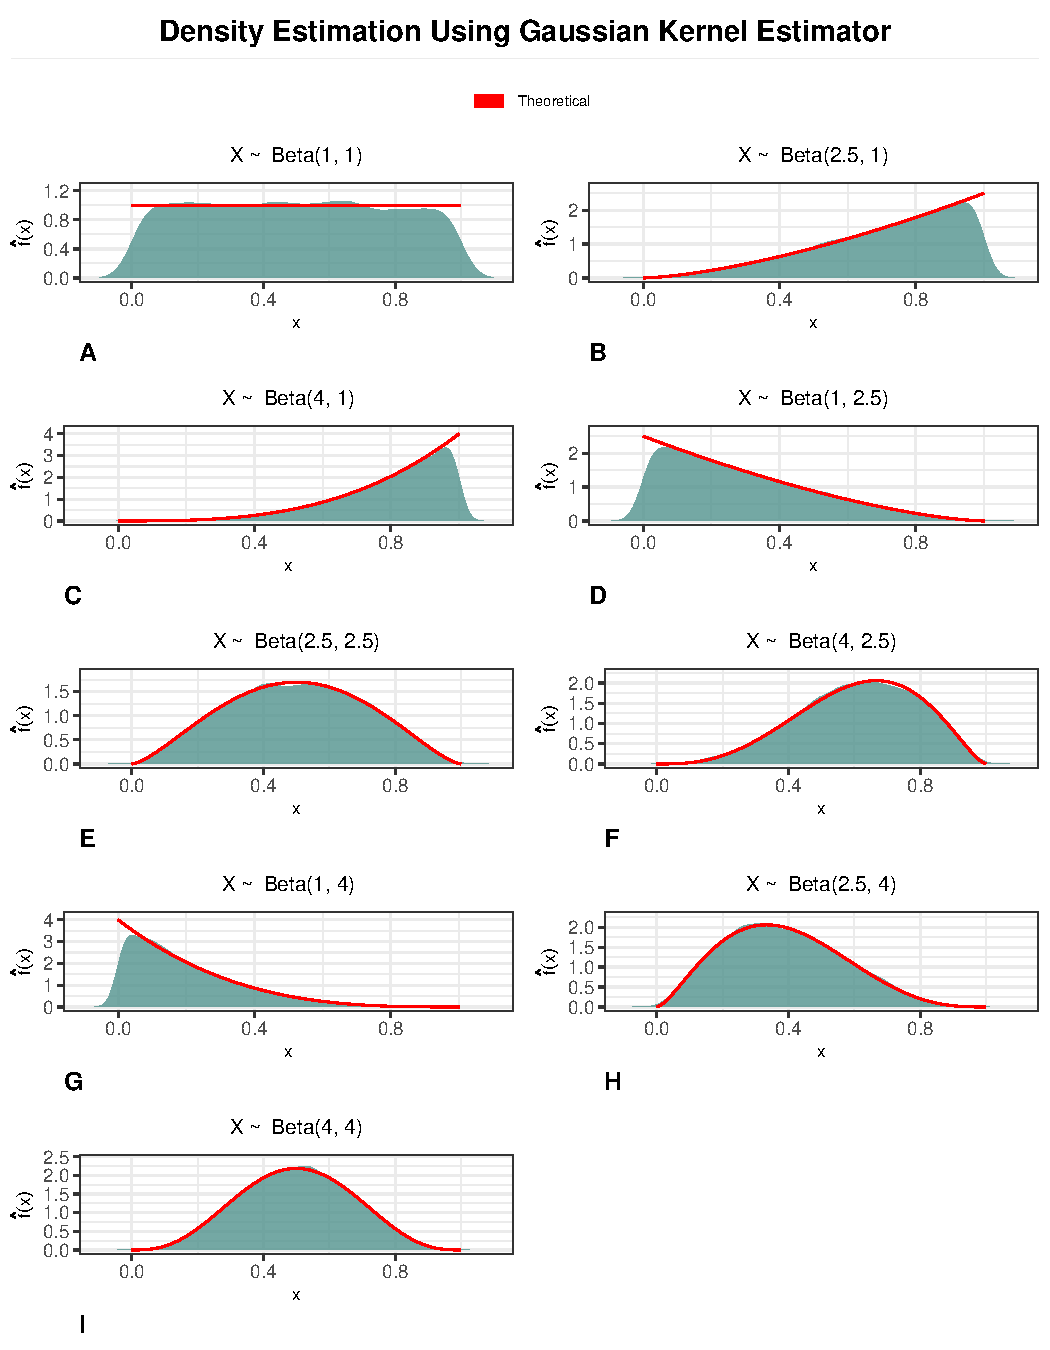
\includegraphics[width=1\linewidth]{thesis_files/figure-latex/unnamed-chunk-40-1} 

}

\caption{\label{fig:trans}}\label{fig:unnamed-chunk-40}
\end{figure}
We see the difference between using the transformation approach versus estimating the density of \(X\) without first transforming it to be unbounded in Figure \ref{fig:original}.
\begin{figure}

{\centering 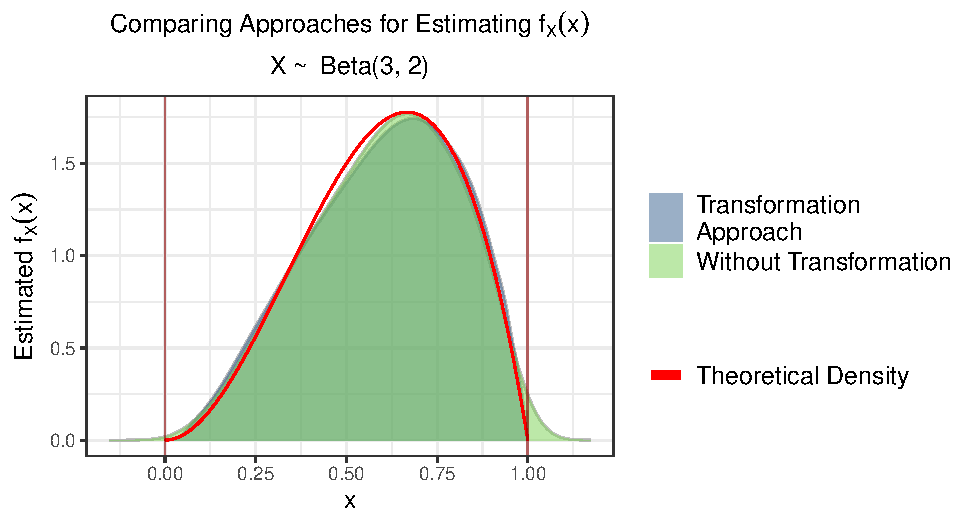
\includegraphics[width=1\linewidth]{thesis_files/figure-latex/create-fig-original-1} 

}

\caption{\label{fig:original}}\label{fig:create-fig-original}
\end{figure}
However, when we simulate densities that have greater mass toward the boundaries 0 or 1, we see that boundary bias becomes problematic (Figure \ref{fig:compare-beta-params}). This is evident in panels B, C, D, and G of Figure \ref{fig:compare-beta-params}, where the estimated density near the boundaries is a poor estimate of the true density.
\begin{figure}

{\centering 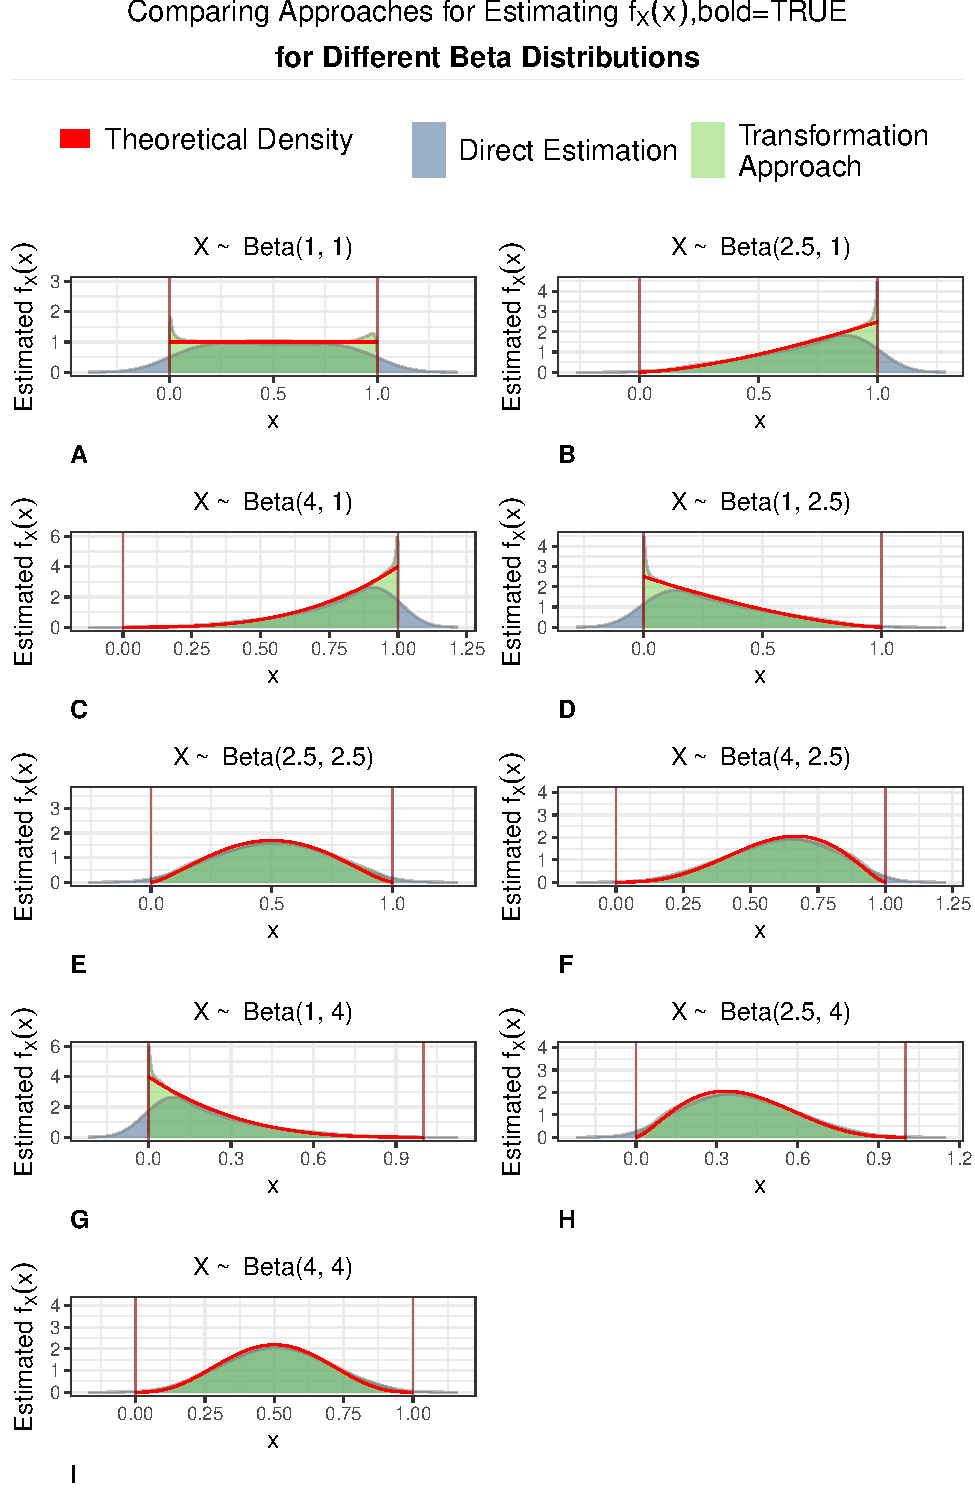
\includegraphics[width=1\linewidth]{thesis_files/figure-latex/unnamed-chunk-42-1} 

}

\caption{\label{fig:compare-beta-params}}\label{fig:unnamed-chunk-42}
\end{figure}
An alternative to the transformation approach for density estimation of bounded variables by using beta kernel estimators, which resolves the issue of boundary bias.

As defined in S. X. Chen (1999), the most simple beta kernel estimator would be
\[\hat f_1(x) = \dfrac{\sum_{i=1}^n K_{x/b + 1, \; (1-x)/b + 1} (X_i)}{n}\]

where \(K_{\text{shape1}, \text{shape2}}\) is the density function \(Beta(shape1, \; shape2)\).

However, S. X. Chen (1999) show that the modified beta kernel estimator \(\hat f_2(x)\) has lower variance and bias than \(\hat f_1\), where we define \(\hat f_2\) as follows:

\[
\hat f_2(x)  = \dfrac{\sum_{i=1}^n K_{x,b}^*(X_i)}{n},\]

\[K^*_{x,b} = \begin{cases}K_{x/b, \; (1-x)/b }(t)  & \text{if }x \in [2b,1-2b] \\
K_{\rho(x), \; (1-x)/b } (t)  & \text{if } x \in [0,2b) \\
K_{x/b, \; \rho(1-x)}(t) & \text{if } x\in(1-2b,1]
\end{cases},
\]
\[\rho(x,b) = 2b^2 + 2.5 - \sqrt{b^2 + 6b^2 +2.25-x^2 -x/b}.\]

Notably, for beta kernel estimators, the shape of the kernel depends on \(x\) (Figure \ref{fig:depends-on-x}).
\begin{figure}

{\centering 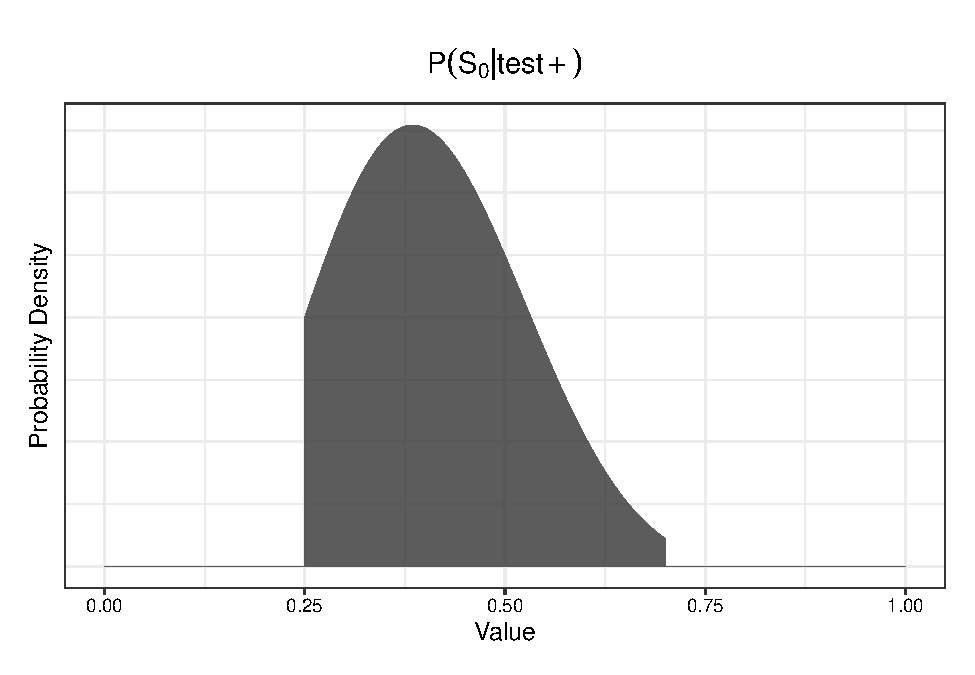
\includegraphics[width=1\linewidth]{thesis_files/figure-latex/unnamed-chunk-45-1} 

}

\caption{\label{fig:depends-on-x}}\label{fig:unnamed-chunk-45}
\end{figure}
As we did in Figure \ref{fig:compare-beta-params}, we can compare the performance of the beta kernel \(\hat f_2\) for estimating the density of samples from different beta distributions (Figure \ref{fig:comp-beta}).
\begin{figure}

{\centering 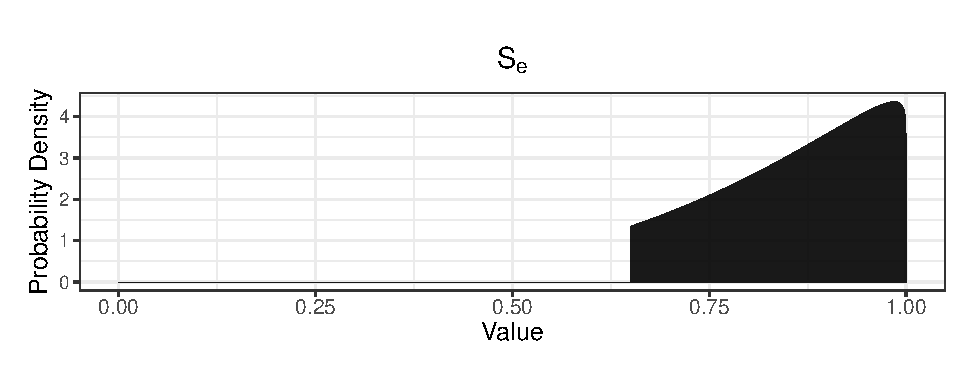
\includegraphics[width=1\linewidth]{thesis_files/figure-latex/unnamed-chunk-47-1} 

}

\caption{\label{fig:comp-beta}}\label{fig:unnamed-chunk-47}
\end{figure}
Although we can see the advantages of using the beta kernel estimator, in practice, available implementations (e.g., the \texttt{bde} package implementation) are much more computationally expensive than using Gaussian kernel density estimation, which make the beta kernel estimator unfeasible for this work. The exact density of the induced distribution is not going to change the estimated counts dramatically relative to the other sources of variability (e.g.~the specification of the prior distributions or sources of data to inform these priors), and, as we see in Figure \ref{fig:gaus}, Gaussian density estimation does perform reasonably well for a variety of bounded distribution shapes.
\begin{figure}

{\centering 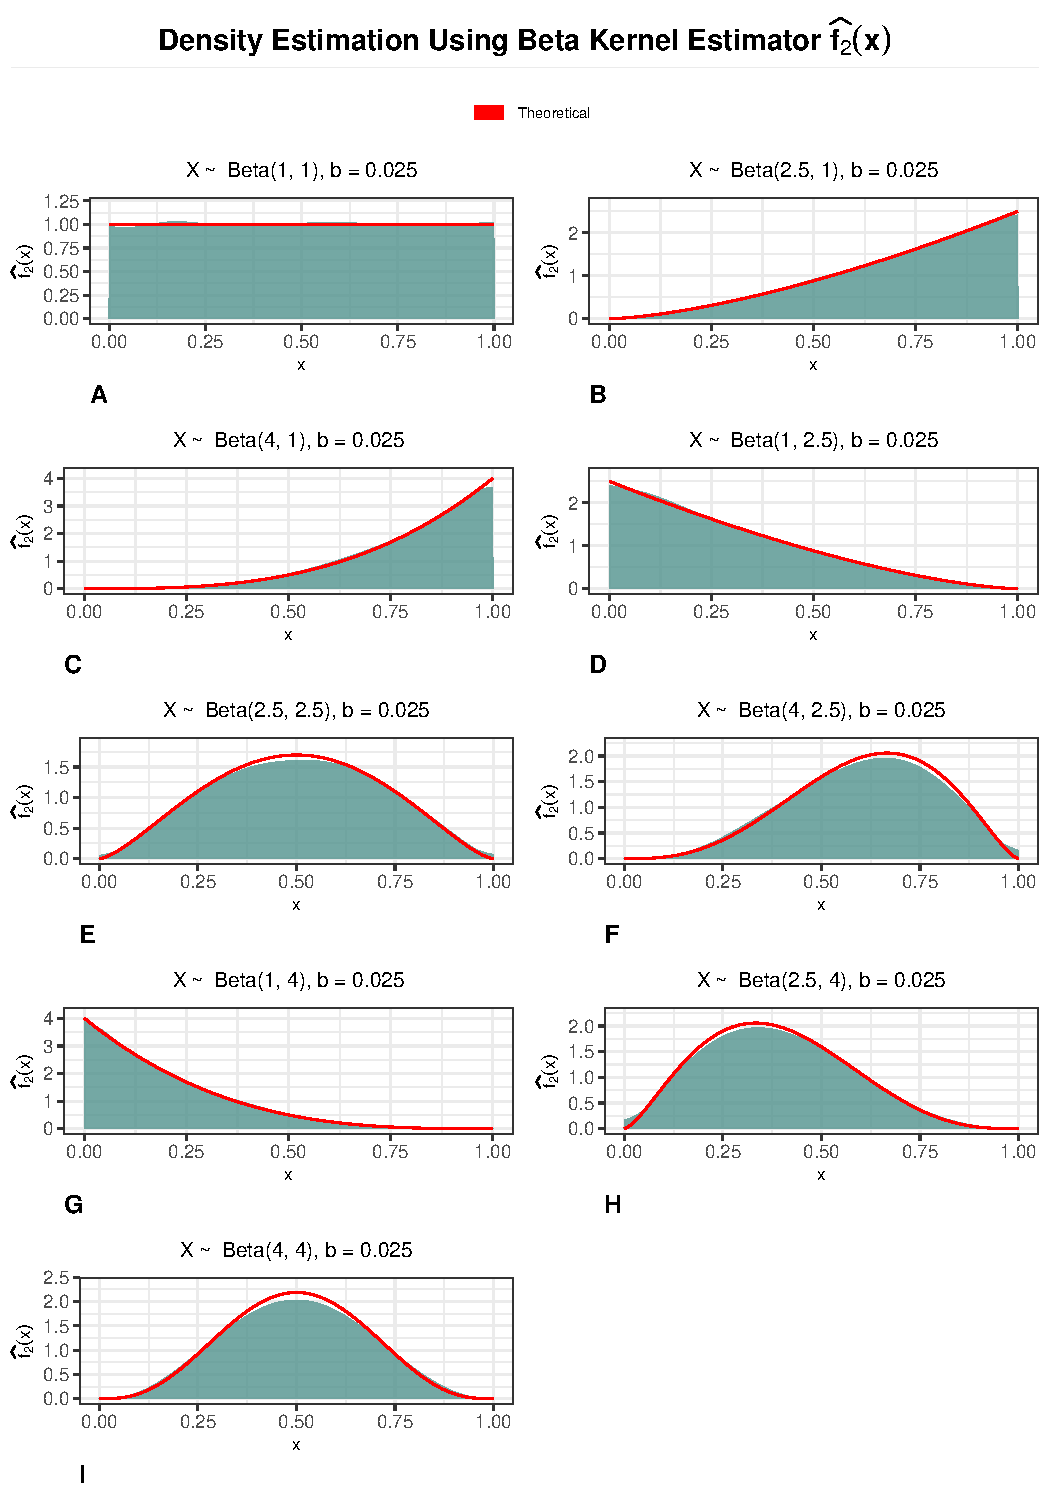
\includegraphics[width=1\linewidth]{thesis_files/figure-latex/unnamed-chunk-48-1} 

}

\caption{\label{fig:gaus}}\label{fig:unnamed-chunk-48}
\end{figure}
\hypertarget{defpriors}{%
\chapter{Definition of Prior Distributions for Bias Parameters}\label{defpriors}}

\hypertarget{background-on-the-beta-distribution}{%
\section{Background on the Beta Distribution}\label{background-on-the-beta-distribution}}

The priors we are specifying here are for probabilities, with the exception of \(\alpha\) and \(\beta\), which represent ratios of probabilities. To define a prior for a parameter that takes on values in \([0,1]\), a particularly useful distribution is the beta distribution, which is only defined on the interval \([0,1]\). It is parameterized by two positive values \(a, b\)\footnote{In R, \(a\) = shape1 and \(b\) = shape2.}.

The beta distribution is an extremely flexible distribution\footnote{The beta distribution is also useful in Bayesian statistics, because it is the conjugate prior distribution for the binomial distribution and negative binomial distributions. That is, if we have a binomial likelihood with parameter \(p\) and \(p\) is distributed according to the beta distribution, the resulting posterior follows a beta distribution.}; by altering the parameters \(a,b\), we can get an extensive array of shapes, as seen below.
\begin{center}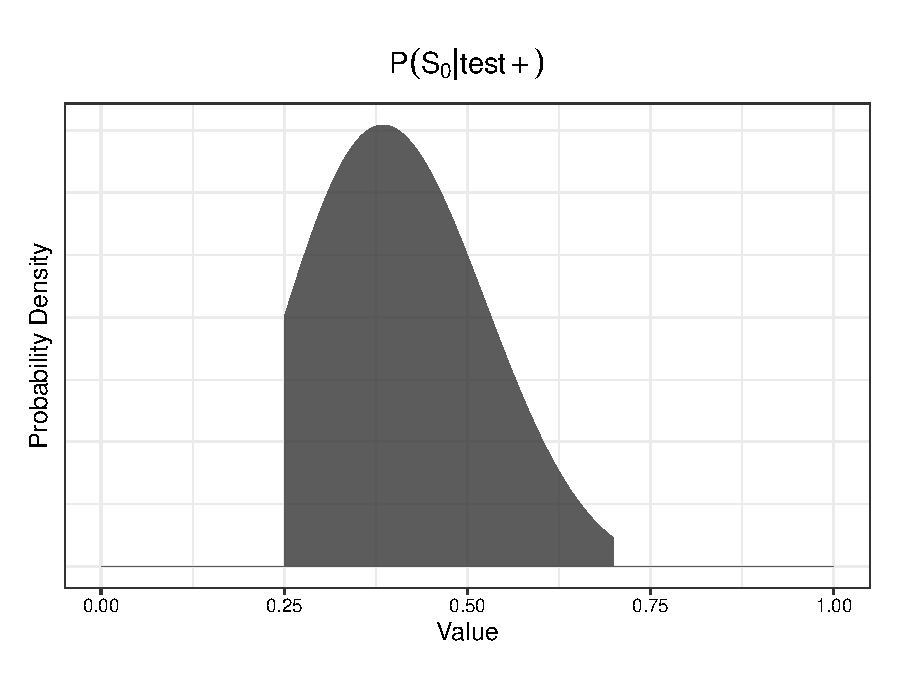
\includegraphics[width=0.9\linewidth]{thesis_files/figure-latex/unnamed-chunk-50-1} \end{center}

In defining a beta distribution to reflect knowledge about a parameter, we need to work backwards to find the parameters \(a\) and \(b\) that correspond to the desired mean and variance.

There are multiple parameterizations of the beta distribution, but R uses that where we define the probability density function as

\[
f(x|a,b) = \dfrac{\Gamma(a + b)}{\Gamma(a) \Gamma(b)} x^{a - 1} (1-x)^{b - 1}.
\]
or equivalently as
\[
f(x|a,\beta) = \dfrac{1}{B(a,b)} x^{a - 1} (1-x)^{b - 1},
\]
where the beta function \(B(a, b) = \dfrac{\Gamma(a)\Gamma(b) }{\Gamma ( a + b)}\).

The expected value of the beta distribution is then \(E(X) = \dfrac{a}{a + b}\) and the variance is given by \(V(X) = \dfrac{a b}{(a + b)^2(a +b + 1)}\); the derivation for both is given in the appendix. We can then solve for \(a\) and \(b\) to obtain \(a = \Big(\frac{1-\mu}{\sigma^2} - \frac{1}{\mu}\Big) \mu^2\) and \(b = \alpha\Big(\frac{1}{\mu} - 1\Big)\). At this point, we can easily write a function in R that generates the parameters of the beta distribution with the desired mean and variance.

\hypertarget{background-on-the-gamma-distribution}{%
\section{Background on the Gamma Distribution}\label{background-on-the-gamma-distribution}}

The gamma distribution is another very flexible distribution. However, the support of the gamma distribution is \((0,\infty)\) rather than \([0,1]\). Because some of the bias parameters are not probabilities (\(\alpha\) and \(\beta\) are ratios of probabilities), we can instead use the gamma distribution to allow the random variable to take on values over 1.

As with the beta distribution, a variety of shapes are possible with the gamma distribution.
\begin{center}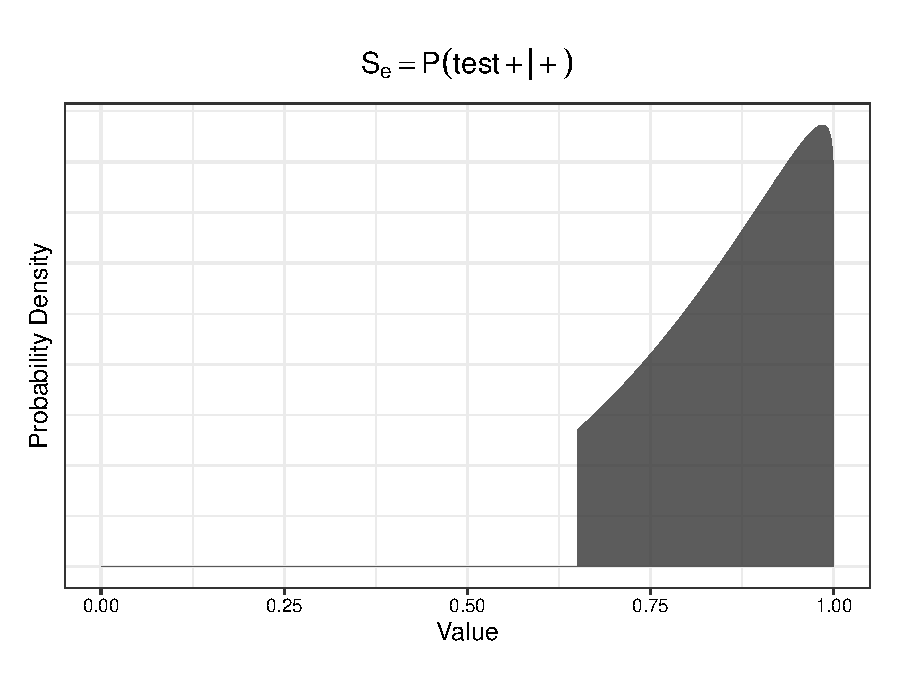
\includegraphics[width=0.9\linewidth]{thesis_files/figure-latex/unnamed-chunk-51-1} \end{center}

Let \(k=shape\) and \(\theta=scale\). The parameterization of the gamma distribution that R uses is

\[f(x|k,\theta) = \frac{1}{\Gamma(k) \;\theta^k}x^{k-1} e^{x/\theta}\]
where the mean \(\mu =k\theta\) and the variance \(\sigma^2 = k\theta^2\).

This allows us to obtain \(\dfrac{\mu^2}{\sigma^2} = \dfrac{k^2 \theta^2}{k\theta^2} = k =shape\).

Then, substituting this result in for \(k\), we have \[\sigma^2 = k \theta^2 = \dfrac{\mu^2}{\sigma^2} \theta^2\]
\[\frac{\sigma^4}{\mu^2}=\theta^2\]

\[\frac{\sigma^2}{\mu}=\theta = scale.\]
This allows us to calculate the shape and scale parameters of a gamma distribution with the desired mean and variance.

\hypertarget{definition-of-prior-distributions-for-incomplete-testing-correction}{%
\section{Definition of Prior Distributions for Incomplete Testing Correction}\label{definition-of-prior-distributions-for-incomplete-testing-correction}}

\hypertarget{defining-ps_1textuntested}{%
\subsection{\texorpdfstring{Defining \(P(S_1|\text{untested})\)}{Defining P(S\_1\textbar\textbackslash text\{untested\})}}\label{defining-ps_1textuntested}}

We recall that \(S_1\) denotes the event that an individual has moderate to severe symptoms, so
\(P(S_1|Untested)\) is the probability of having moderate to severe symptoms among those who were not tested. We note that this would include people that have moderate to severe COVID-like symptoms that do indeed have COVID-19 as well as people that do not have COVID-19 and have some other respiratory illness.

Wu et al.~(2020) defined this distribution such that \(P(S_1|\text{untested}) \sim TBeta(\alpha = 1.18, \beta = 45.97)\), bounded between 0 and 15\%, as we see below. When we define the distribution of \(P(S_1|\text{untested})\), we release the truncation. Furthermore, we actually remove the truncation on all prior distributions considered. This choice was based on the fact that we have a lack of data to support particular bounds for a truncated distribution, and such assumptions can lead to difficulties in the Bayesian melding component of the probabilistic bias analysis.
\begin{center}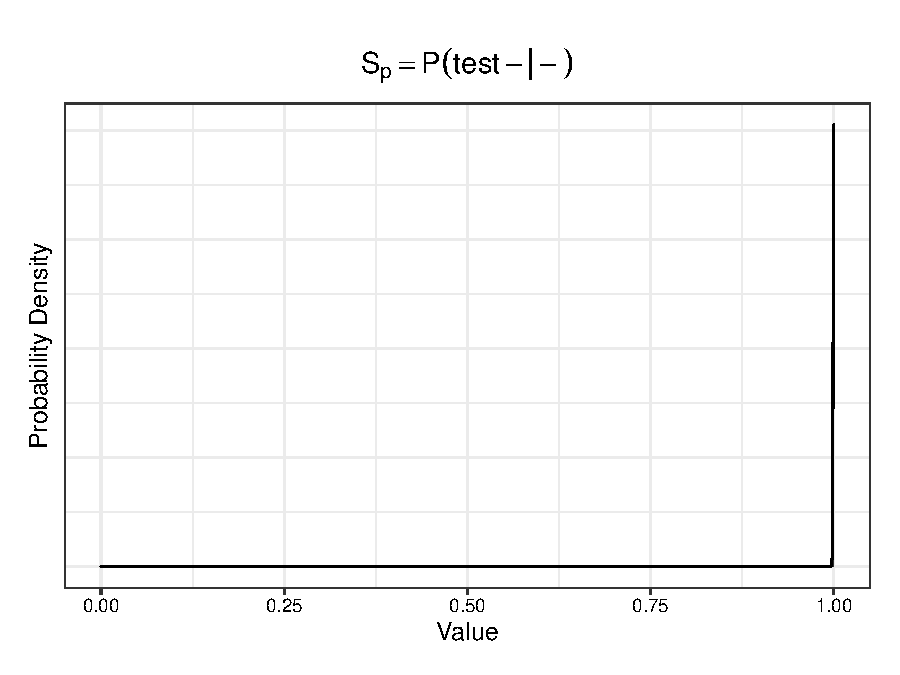
\includegraphics[width=1\linewidth]{thesis_files/figure-latex/unnamed-chunk-54-1} \end{center}

However, to implement this approach over a more extended time interval, we need to allow this parameter to vary by time. Due to state-specific differences in symptom prevalence, it also makes more sense to allow this parameter to vary by state.

To do this, we can use the COVID-like illness indicator from the COVID-19 Trends and Impact Survey (Salomon et al., 2021a). The COVID-19 Trends and Impact Survey (CTIS) is a large scale internet-based survey that invites a sample of Facebook users to respond to questions on several topics of public health interest, including testing and symptom status. The survey effort selects participants using stratified random sampling by state, and responses are aggregated and made publicly available.

Below, we see that the distribution of the proportion of the population with COVID-like illness over all of 2021 is in a similar range as the distribution defined for \(P(S_1|untested)\), with the bulk of the distribution between 0 and 15\%, although the COVID-19-like-illness has more density toward zero.
\begin{center}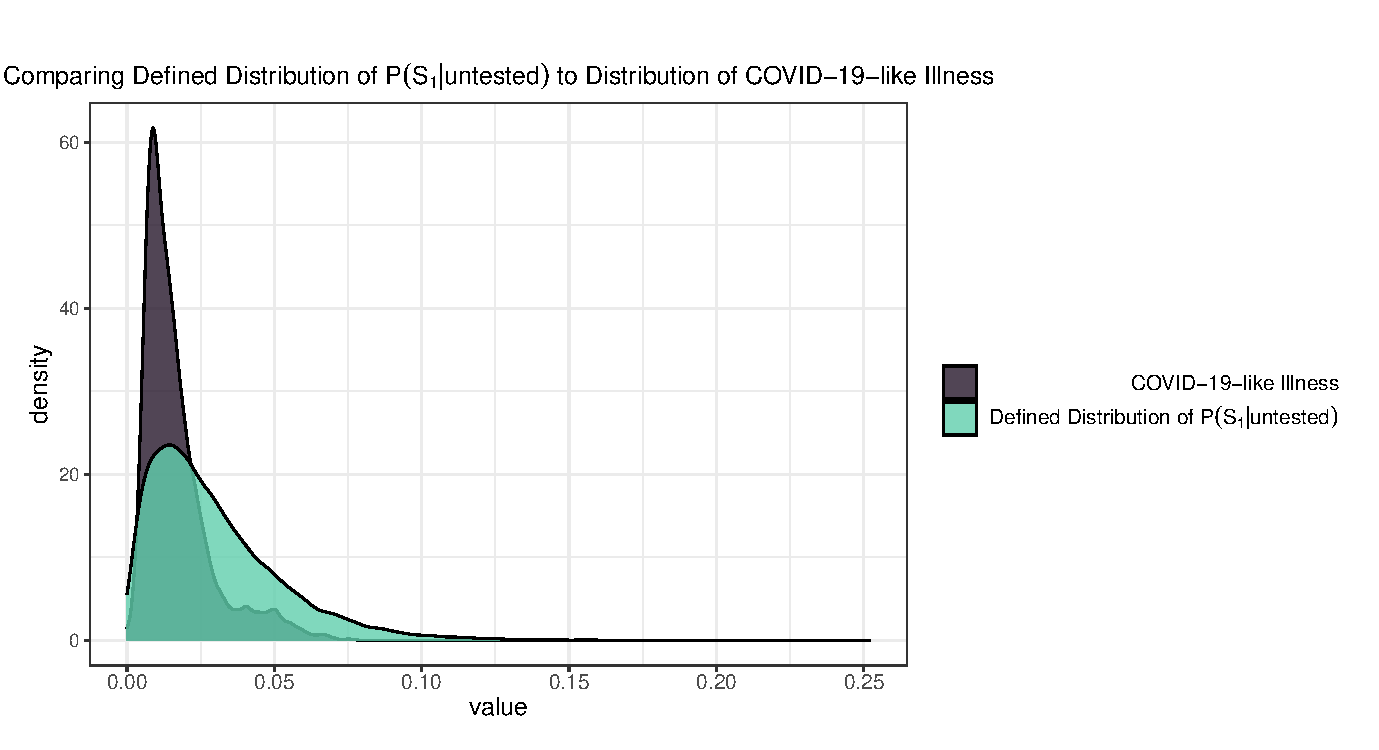
\includegraphics[width=0.8\linewidth]{figure/emp_p_s_untested} \end{center}

\hypertarget{defining-alpha}{%
\subsection{\texorpdfstring{Defining \(\alpha\)}{Defining \textbackslash alpha}}\label{defining-alpha}}

We define \(\alpha\) as the ratio \(\frac{P(\text{test}_+|S_1, \text{untested})}{P(test+|\text{tested})}\), applied to allow
\(P(\text{test}_+|S_1, \text{untested})\) to vary by state. \(P(\text{test}_+|\text{tested})\) is the state-level empirical estimate, but we do not calculate \(\alpha\) itself using the state-level empirical estimate. Instead, we calculate \(P(\text{test}_+|S_1, \text{untested})\) as \(P(\text{test}_+|S_1, \text{untested}) =\alpha P(\text{test}_+|\text{tested})\). We can think about \(\alpha\) as the adjustment to the test positivity rate as we estimate the probability of testing positive among symptomatic \emph{untested} individuals. We assume this ratio is close to 1, that is, that the probability of testing positive among symptomatic untested individuals would be near 90\% of the probability of testing positive among tested individuals (not all of whom would be symptomatic).

With the the expansion of testing resources in 2021, it is plausible that \(P(\text{test}_+|\text{untested},S_1)\) could exceed \(P(\text{test}_+|\text{tested})\), so we use a gamma distribution to allow \(\alpha\) to take on values greater than 1.
\begin{center}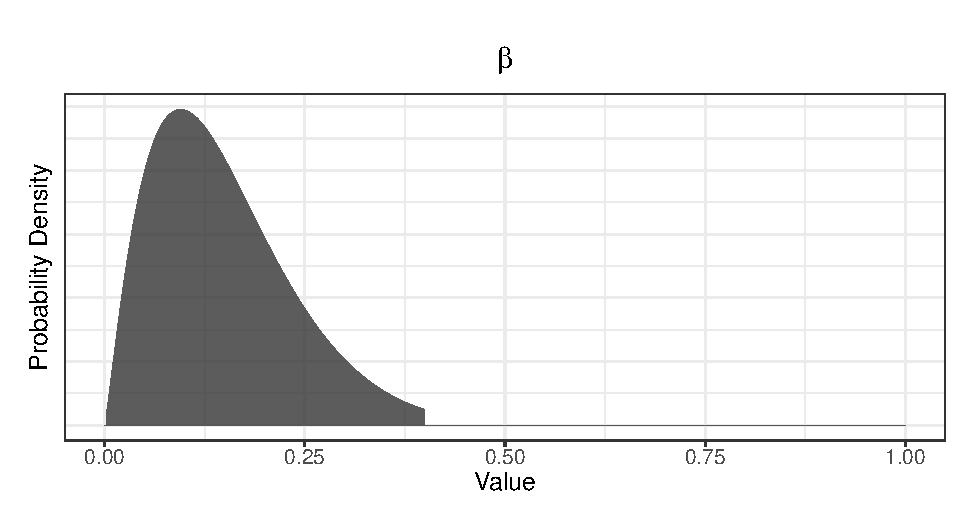
\includegraphics[width=0.8\linewidth]{thesis_files/figure-latex/unnamed-chunk-57-1} \end{center}

\hypertarget{defining-beta}{%
\subsection{\texorpdfstring{Defining \(\beta\)}{Defining \textbackslash beta}}\label{defining-beta}}

Similar to the way we defined \(\alpha\), we define \(\beta\) as the ratio of \(\dfrac{P(\text{test}_+ |S_0, \text{untested})}{P(\text{test}_+|\text{tested})}\), applied to allow \(P(\text{test}_+ |S_0, \text{untested})\) to vary by state. We use \(\beta\) to calculate \(P(test+|S_1, \text{untested})\) by the expression \(P(\text{test}_+|S_0, \text{untested}) =\beta P(\text{test}_+|\text{tested})\). We can think about \(\beta\) as the adjustment to the test positivity rate as we estimate the probability of testing positive among aymptomatic untested individuals (in contrast to \(\alpha\), which is symptomatic untested individuals). We assume the values of \(\beta\) are substantially lower than \(\alpha\), reflecting that we expect a much smaller proportion of asymptomatic untested individuals to test positive than symptomatic individuals.
\begin{center}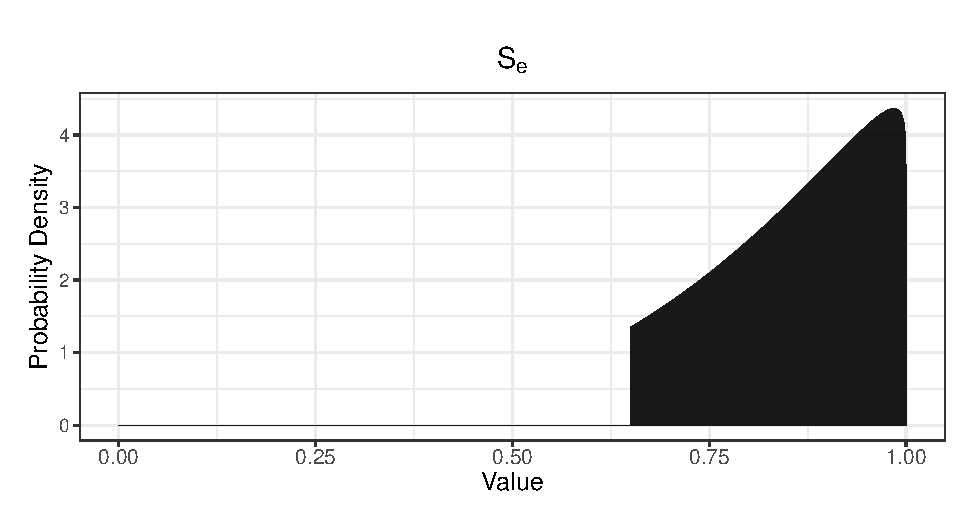
\includegraphics[width=0.8\linewidth]{thesis_files/figure-latex/unnamed-chunk-58-1} \end{center}

Because we define \(\beta\) as the ratio of \(\frac{P(\text{test}_+ |S_0, \text{untested})}{P(\text{test}_+|\text{tested})}\), we can estimate \(\beta\) empirically by taking the screening test positivity rate as an estimate of \(P(test + |S_0, untested)\) and then dividing by the overall test positivity rate \(P(\text{test}_+|\text{tested})\). State-level estimates for screening test positivity and overall test positivity are available through the COVID-19 Trends and Impact Survey, enabling us to obtain a time and state-specific estimate of \(\beta\).

\hypertarget{defining-ps_0texttest_textuntested}{%
\subsection{\texorpdfstring{Defining \(P(S_0|\text{test}_+,\text{untested})\)}{Defining P(S\_0\textbar\textbackslash text\{test\}\_+,\textbackslash text\{untested\})}}\label{defining-ps_0texttest_textuntested}}

\(P(S_0|\text{test}_+)\) is the probability of not having symptoms among those who test positive, that is, the asymptomatic rate of COVID-19.

One large meta-analysis found \(P(S_0|test+)\) to be 40.50\% (95\% CI: 33.50\%-47.50\%), although it did not restrict to screening studies (Ma et al., 2021a). Another meta-analysis, when restricting to screening studies, found \(P(S_0|test+)\) to be 47.3\% (95\% CI: 34.0\% -61.0\%) (Sah et al., 2021a).
\begin{center}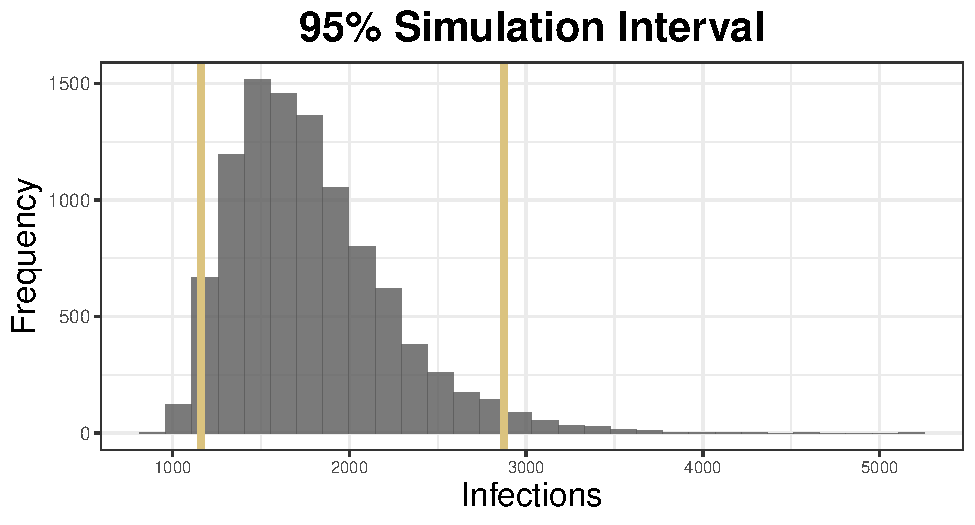
\includegraphics[width=0.8\linewidth]{thesis_files/figure-latex/unnamed-chunk-59-1} \end{center}

\hypertarget{definition-of-priors-for-test-inaccuracy-correction}{%
\section{Definition of Priors for Test Inaccuracy Correction}\label{definition-of-priors-for-test-inaccuracy-correction}}

\hypertarget{defining-test-sensitivity-s_e}{%
\subsection{\texorpdfstring{Defining Test Sensitivity (\(S_e\))}{Defining Test Sensitivity (S\_e)}}\label{defining-test-sensitivity-s_e}}

We define the the test sensitivity and test sensitivity to follow the definitions in Wu et al. (2020b).
\(S_e\) is defined such that \(S_e \sim TBeta(\alpha = 4.20, \beta = 1.05)\), bounded between 0.65 and 1 and with mean \(\dfrac{\alpha}{\alpha + \beta} = 0.80\).
\begin{center}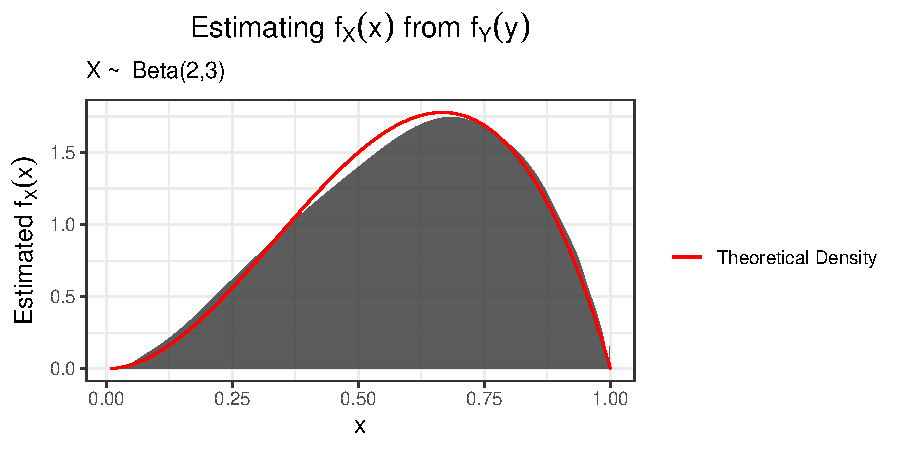
\includegraphics[width=0.8\linewidth]{thesis_files/figure-latex/unnamed-chunk-60-1} \end{center}

\textbf{Data available for informing this prior distribution:}

In a population-based retrospective study including both inpatients and outpatients, the clinical sensitivity was estimated to be 89.9\% (95\% CI 88.2 -- 92.1\%) by considering repeat-tested patients who initially tested negative but later tested positive (Kortela et al., 2021). However, as Kortela \emph{et al.} discussed, this approach is likely an overestimate of the true clinical sensitivity, because individuals will only be tested twice if there is high clinical suspicion that they do have COVID-19. To account for this, they produced an estimate of sensitivity including cases with high clinical suspicion in the denominator, which resulted in an estimate closer to 50\%, yet this is likely an underestimate due to the fact that even those with a classical COVID-19 symptom presentation may not have COVID-19. They concluded that due to these biases, the true value most likely falls between the overestimate near 90\% and the underestimate near 50\%.

Another analysis of repeat-tested patients using data from a large sample of patients tested at the provincial Public Health Laboratory in Canada estimated the clinical sensitivity to be 90.7\% (95\% CI 82.6--98.9\%) (Kanji et al., 2021). Green \emph{et al.} found that the clinical sensitivity ranged from 58\% to 96\%: the estimate of 96\% was dependent on the assumption that negative results, repeated or not, were true negatives, while the estimate of 58\% assumed the rate of false negatives among the repeat-tested population would be the same as in the repeat-tested patients (Green et al., 2020). In a meta-analysis of 51 studies, Mustafa \emph{et al.} found a pooled estimate of the clinical sensitivity as 0.96 (95\% CI 93\% - 98\%) (Mustafa Hellou et al., 2021).

Because PCR tests are designed to target a highly conserved region of the viral genome, their sensitivity was expected to be relatively robust to the circulation of different variants of SARS-CoV-2. However, analytical sensitivity has shown some differences by genetic variants (Y. Chen et al., 2022). Viral shedding dynamics also have differed by genetic variant, but the variants dominant throughout most of the time period considered here, Delta and Omicron, have similar viral loads (Fall et al., 2022; Singanayagam et al., 2022).
\begin{figure}

{\centering 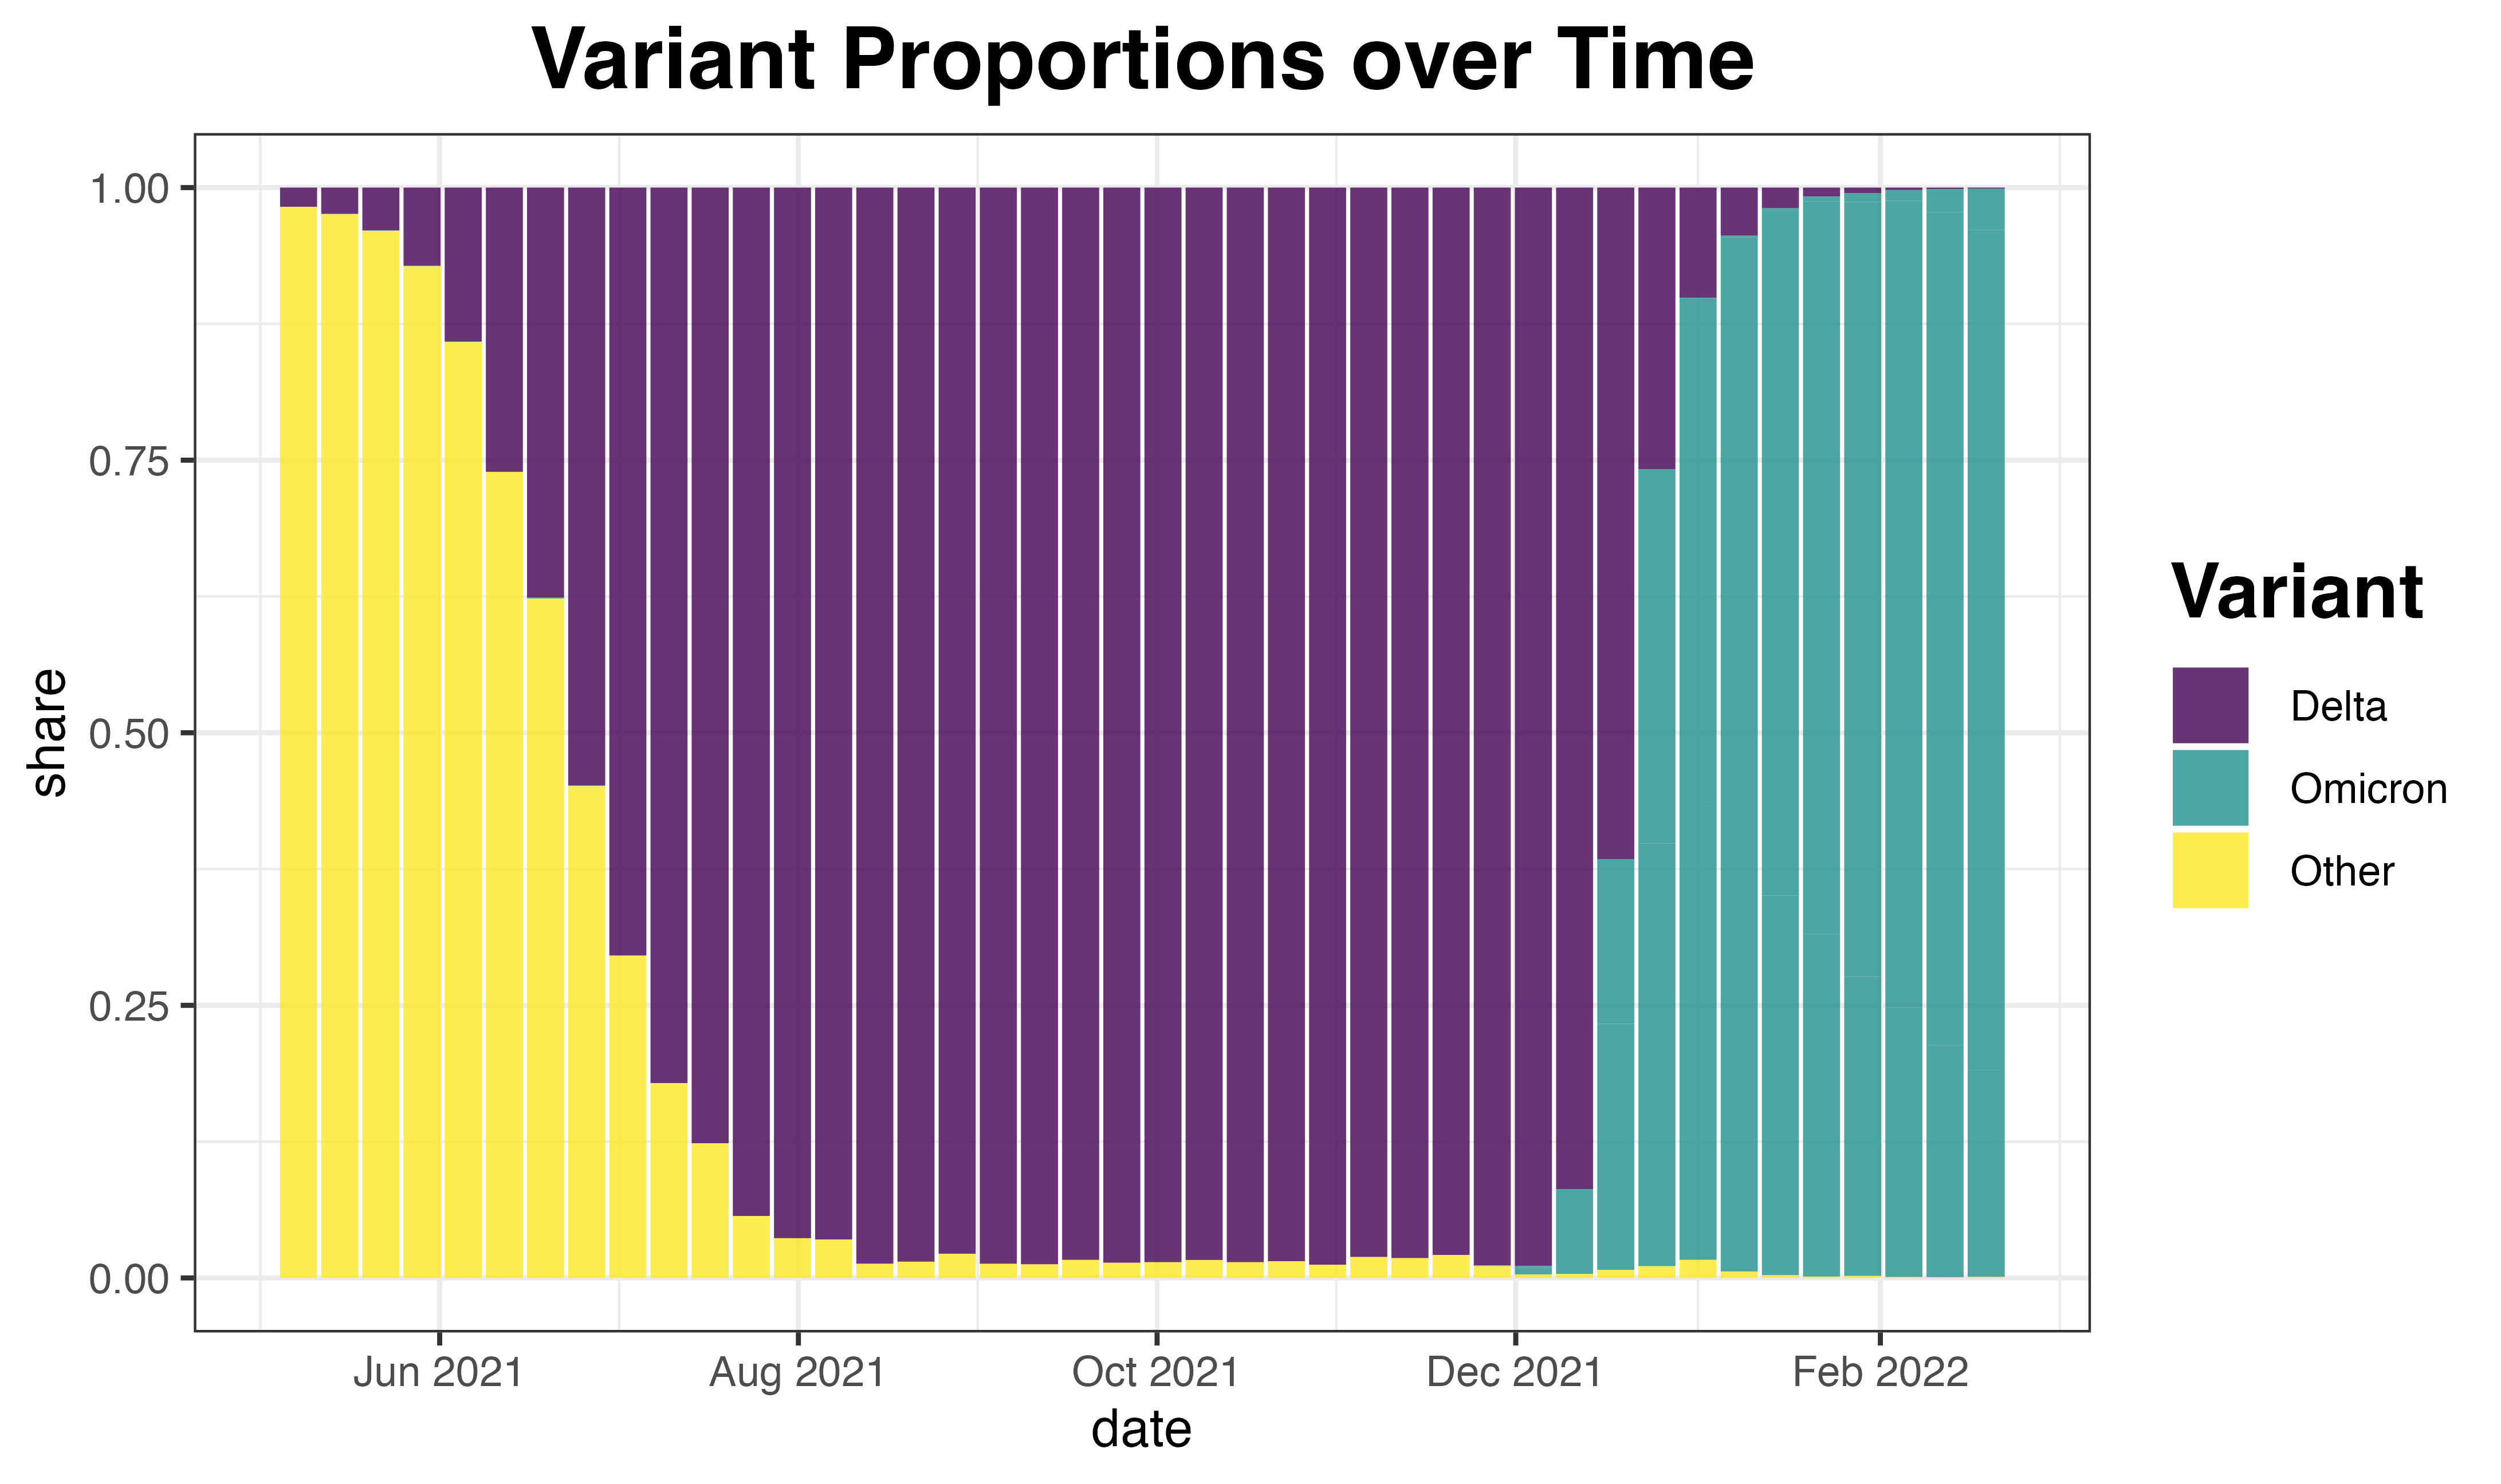
\includegraphics[width=0.8\linewidth]{./figure/variant_plot} 

}

\caption{Variant proportions in the United States from genomic surveillance data collected by the CDC. Data is not available for time periods earlier than May 8, 2021.}\label{fig:unnamed-chunk-62}
\end{figure}
Ultimately, although it is plausible that test sensitivity may vary by time due to differences in viral shedding dynamics over time as well as differences due to the mutations present in circulating variants, there is a lack of data to inform exactly how the sensitivity may vary over time. As a result, we assume the test sensitivity is independent and identically distributed across time periods.

\hypertarget{defining-test-specificity-s_p}{%
\section{\texorpdfstring{Defining Test Specificity (\(S_p\))}{Defining Test Specificity (S\_p)}}\label{defining-test-specificity-s_p}}

The test specificity \(P(\text{test negative}| \text{negative})\) is defined as \(P(\text{test negative}| \text{negative}) \sim TBeta(a = 4998.50, \beta = 0.25)\), bounded between 0.9998 and 1 and with mean \(\dfrac{a}{a + b} = 0.99995\). The high certainty for this parameter is based on the CDC 2019-nCoV Real-Time RT-PCR Diagnostic Panel.
\begin{center}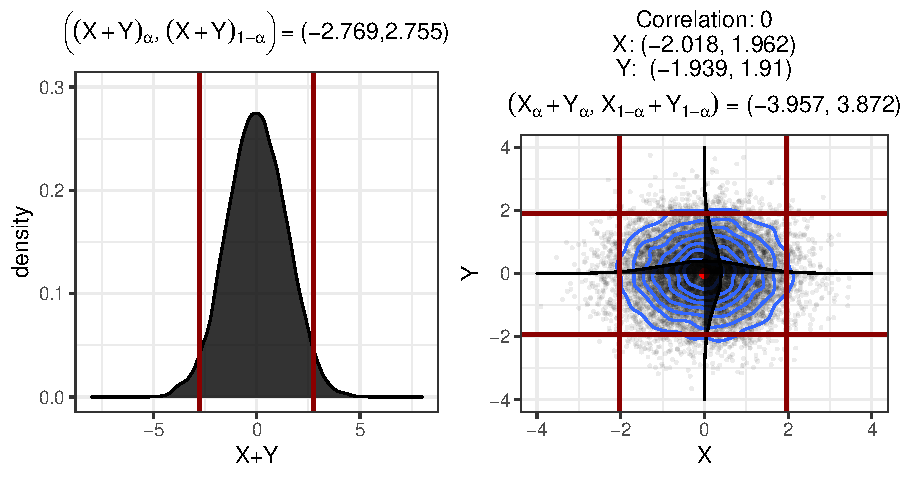
\includegraphics[width=0.8\linewidth]{thesis_files/figure-latex/unnamed-chunk-63-1} \end{center}

\hypertarget{exploration-of-the-implications-of-changes-in-the-bias-parameters}{%
\section{Exploration of the Implications of Changes in the Bias Parameters}\label{exploration-of-the-implications-of-changes-in-the-bias-parameters}}

To explore the implications of changes in the bias parameter distributions both on the melding and the final corrected estimates, we developed the Shiny app hosted \href{https://q-w-a.shinyapps.io/bayesian_melding_priors/}{here}.\footnote{Code is available at the repository \href{https://github.com/q-w-a/probabilistic_bias_correction}{here}}.

\hypertarget{correction-for-incomplete-testing}{%
\section{Correction for Incomplete Testing}\label{correction-for-incomplete-testing}}

We denote \(N^*\) to be positive tests (not infections).

As discussed previously, once we have sampled values from the constrained distributions of \(P(S_1|untested)\), \(\alpha\), \(\beta\), we estimate the test positivity among the symptomatic untested population as \(P(+|S_1,untested) = \alpha \; P(test +|tested)\), and we estimate the test positivity among the asymptomatic untested population as \(P(+|S_0,untested) = \beta \; P(test +|tested)\). Then, we compute the positives among the symptomatic and mild/asymptomatic parts of the population respectively as

\[N^*_{\text{untested},S_1} = N_{\text{untested}} \; P(S_1|\text{untested}) \cdot P(\text{test}_+ | S_1,\text{untested}) \;\;\;\text{ and }\]
\[N^*_{\text{untested},S_0} = N_{\text{untested}}(1-P(S_1|\text{untested}))P(test + | S_0,\text{untested}).\]
Then, we take the total positives among the untested population as

\[N^*_{\text{untested}} = N^*_{\text{untested},S_1} + N^*_{\text{untested},S_0}\]
and finally we add the number of observed positives, \(N^*_{tested}\) to obtain the estimate for the positives among the total population, as

\[N^* = N^*_{\text{untested}} +N^*_{\text{untested}}.\]

\hypertarget{correct-test-inaccuracy}{%
\section{Correction for Diagnostic Test Inaccuracy}\label{correct-test-inaccuracy}}

At this point, we have corrected for the incompleteness of testing. That is, we have an estimate of who would have tested positive if we tested the entire population. However, we also need to correct for imperfect test accuracy.

Test accuracy is broken up into two components, specificity and sensitivity.

We define test sensitivity and specificity as follows:
* \(S_e\) = test sensitivity = the probability an individual tests positive if they have COVID-19 (probability of a true positive), that is, \(P(\text{test}_+ | +)\).
* \(S_p\) = test specificity = probability an individual tests negative if they do not have COVID-19 (probability of a true negative), that is, \(P(\text{test}_- |-)\).

Then, given that we have the number \(N^+\) who tested positive (or, in the context of this work, would have tested positive), the specificity \(S_p\), the sensitivity \(S_e\), and the total population size \(N\), we can calculate the true positives with the formula
\[\text{Number Truly Positive} = \dfrac{N^* - (1-S_p) \times N}{S_e+S_p-1}\]
from Modern Epidemiology (Rothman et al., 2008).

\hypertarget{derivation-of-formula-for-correction-for-diagnostic-test-inaccuracy}{%
\subsection{Derivation of Formula for Correction for Diagnostic Test Inaccuracy}\label{derivation-of-formula-for-correction-for-diagnostic-test-inaccuracy}}

We define test sensitivity and specificity as follows:
* \(S_e\) = test sensitivity = the probability an individual tests positive if they have COVID-19 (probability of a true positive), that is, \(P(test + | +)\).
* \(S_p\) = test specificity = probability an individual tests negative if they do not have COVID-19 (probability of a true negative), that is, \(P(test - |-)\).

As defined previously, \(S_e \sim TBeta(0.65, 1)\) and \(S_p \sim TBeta(0.998, 1)\).

To correct case counts for diagnostic test inaccuracy, we use the formula
\[\text{Number Truly Positive} = \dfrac{N^*- (1-S_p) \times N}{S_e+S_p-1}\]
as defined in Rothman et al.~(2008).

To obtain this formula, we let:
\begin{itemize}
\tightlist
\item
  \(N\) denote the total population size
\item
  \(N^*\) denote the number \emph{classified} as positive
\item
  \(N^-\) denote the number \emph{classified} as negative
\item
  \(T^+\) denote the number that is \emph{truly} positive
\item
  \(T^-\) denote the number that is \emph{truly} positive
\end{itemize}
We also recall that
\[ \text{Sensitivity} = S_e = P(test + | +) \]
\[ \text{Specificity} = S_p = P(test - | - ) \]

The quantity we want to estimate is the number of truly positive individuals when accounting for imperfect test accuracy, that is, \(T^+\).

The number classified as positive, \(N^+\) can be written as

\[ N^* = P(test + | +) T^+ + P(test + | -) T^-\]

where \(P(test + | +) T^+\) is the number of true positives and \(P(test + | -) N^-\) is the number of false positives. By the definitions of sensitivity \(S_e\) and specificity \(S_p\) we can write this more clearly as
\[ N^* =S_e T^+ + (1-S_p) T^-.\]

Meanwhile, the number classified as negative, \(N^-\) can be written as

\[ N^- = P(test - | -) T^- + P(test - | +) T^+\]

where \(P(test - | -) T^-\) is the number of true negatives and \(P(test - | +) T^+\) is the number of false negatives. Substituting in \(S_e\) and \(S_p\) we can express this as

\[ N^- = S_p T^- + (1-S_e) T^+.\]

At this point, we can solve the expression \(N^- = S_p T^- + (1-S_e) T^+\) for the number of people classified as positive for the number truly negative, \(T^-\). This yields

\[\dfrac{( N^- - (1-S_e) T^+) }{S_p}=  T^- .\]

Now, we can substitute this result into our expression for \(N^+ =S_e T^+ + (1-S_p) T^-\) and solve for the desired value, the number of truly positive individuals, \(T^+\). This gives us

\[
 N^* =S_e T^+ + (1-S_p)  \left( \dfrac{( N^- - (1-S_e) T^+) }{S_p} \right)
\]

\[
 S_p \; N^* =S_pS_e T^+ + (1-S_p)  \left( {( N^- - (1-S_e) T^+) } \right)
\]

\[
 S_p \; N^* =S_pS_e T^+ + (1-S_p)  ( N^-)  - (1-S_p)(1-S_e) T^+
\]

\[
 S_p \; N^* -   (1-S_p)  ( N^-) =S_pS_e T^+  - (1-S_p)(1-S_e) T^+
\]

\[
 S_p N^* -   (1-S_p)  ( N^-) = (S_pS_e  - (1-S_p)(1-S_e)) T^+
\]

\[
 S_p \; N^* -   (1-S_p)  ( N^-) = (S_p + S_e - 1) T^+
\]

\[
 T^+ = \dfrac{ S_p \; N^* -   (1-S_p)  ( N^-)}{(S_p + S_e - 1)} 
\]

At this point we can simplify the numerator as follows by using the fact \(N =N^* + N^-\). This gives us
\begin{align*} =S_p \;N^* -   (1-S_p)  N^-\\
=  S_p   N^* + S_p  N^- - N^-\\
=  S_p(N^* +  N^-) - N^- \\
=  S_pN - (N-N^*) \\
=  S_pN - (N-N^*) \\
=  (S_p-1)N + N^* \\
=  N^* - (1-S_p)N\\
\end{align*}
so we have
\[
 T^+ = \dfrac{ N^*- (1-S_p)N}{(S_p + S_e - 1)}.
\]

\hypertarget{details-of-implementation}{%
\chapter{Details of Implementation}\label{details-of-implementation}}

To make the implementation more concrete, we will illustrate the steps of the probabilistic bias analysis with the infections in Suffolk County, Massachusetts in from May 9, 2021 to May 23, 2021.

\hypertarget{version-1-priors-do-not-vary-by-state-or-date}{%
\section{Version 1: Priors do Not Vary by State or Date}\label{version-1-priors-do-not-vary-by-state-or-date}}

As we did in the \protect\hyperlink{sampling}{Background} section, we denote the sample size as \(m\) and the posterior (resample) size as \(r\).

We begin by sampling \(m\) times from the defined prior distributions \(\theta = \Big\{ \alpha, \beta, P(S_1| \text{untested})\Big\}\), as we see in Figure \ref{fig:sample-priors}.
\begin{figure}
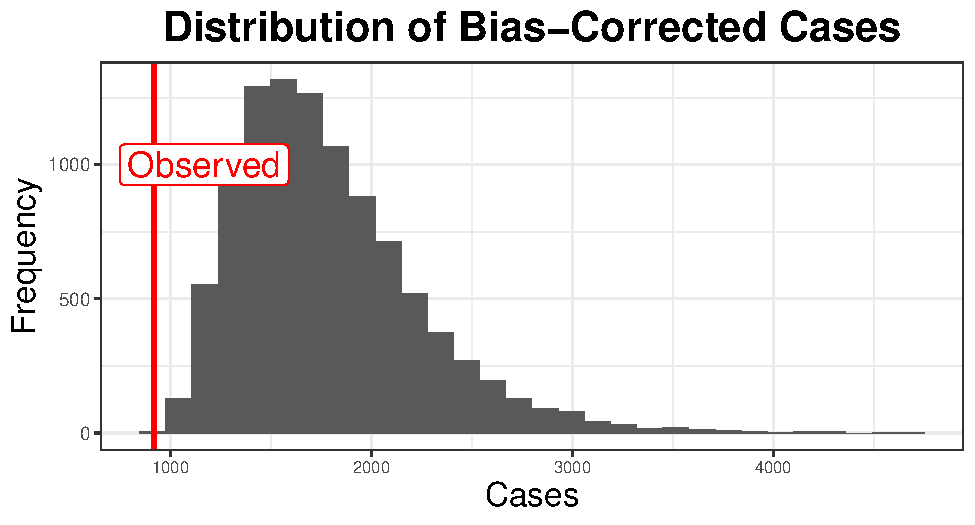
\includegraphics[width=1\linewidth]{thesis_files/figure-latex/unnamed-chunk-67-1} \caption{\label{fig:sample-priors}}\label{fig:unnamed-chunk-67}
\end{figure}
At this point, we use Bayesian melding to obtain \(r\) observations from the constrained priors for \(\alpha, \; \beta, \;P(S_1|\text{untested})\), and \(P(S_0|\text{test}_+,\text{untested})\).

We also sample \(r\) values from the priors for sensitivity and specificity, which we use to correct for imperfect testing accuracy. However, these parameters are not involved in the Bayesian melding.

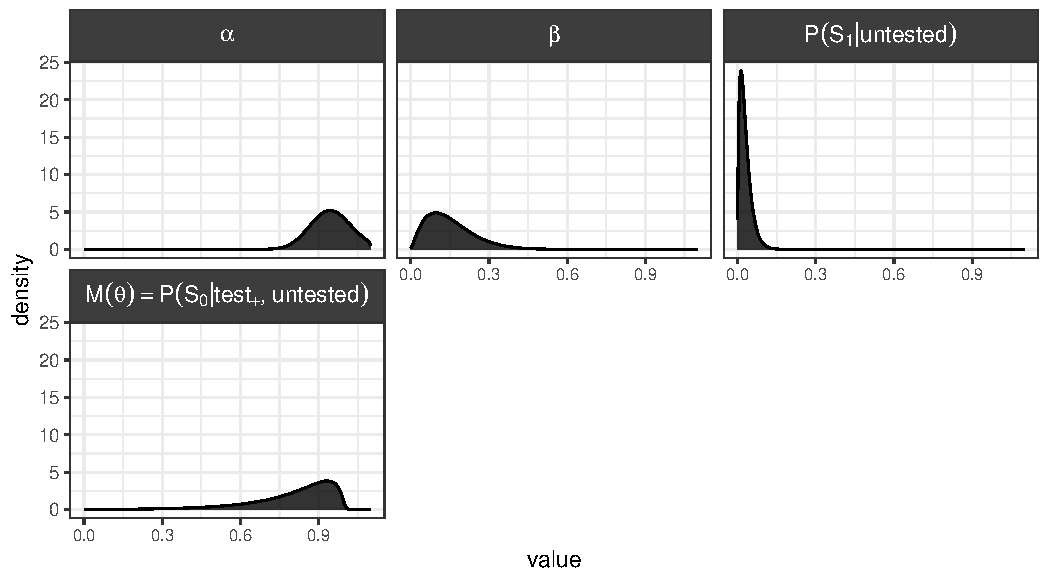
\includegraphics[width=1\linewidth]{thesis_files/figure-latex/unnamed-chunk-68-1}

From here, we obtain the bias corrected estimates by sampling from the \(r\) observations of the bias parameters and computing the unobserved infections.

For example, suppose we sample a value from each of \(\beta,\alpha,P(S_1|\text{untested}), S_p\) and \(S_e\).

We first compute the number of untested individuals as the population size \(N\) minus the number of individuals tested:

\[ N_{\text{untested}} =  N - N_{\text{tested}} .\]

We then use \(\alpha\) and \(\beta\) to estimate the test positivity rates of the symptomatic and asymptomatic partitions of the population, giving us the positivity rates
\[ P( \text{test}_+ | S_1, \text{untested})  = P( \text{test}_+ | \text{tested}) \cdot  \alpha  \]
and
\[ P( \text{test}_+ | S_0, \text{untested})  = P( \text{test}_+ | \text{tested}) \cdot  \beta. \]

We use these positivity rates to calculate the number of positive tests among the untested as
\begin{align*}
N^*_{\text{untested},S_1} &= P( \text{test}_+ | S_1, \text{untested}) ( N_{S_1,\text{untested}}) \\
&= P( \text{test}_+ | S_1, \text{untested}) (N_{\text{untested}} ) P(S_1|\text{untested})\\
N^*_{\text{untested},S_0} &= P( \text{test}_+ | S_0, \text{untested}) ( N_{S_0,\text{untested}})\\
&== P( \text{test}_+ | S_1, \text{untested}) (N_{\text{untested}} ) (1- P(S_1|\text{untested}))
\end{align*}
We use \(N^*\) to denote the number of people who would test positive, not the number who are infected. This distinction is important because we are not yet correcting for diagnostic test inaccuracy. With this notation, \(N^*_{\text{untested}}\) is the number of people among the untested population we expect to test positive if they were all tested, while \(N^*_{\text{tested}}\) is simply the number of positive tests reported for this 2-week interval. This means we can write the total number of individuals who we expect to test positive as
\begin{align*}
 N^*_{\text{untested}}
 &= N^*_{\text{tested}} + N^*_{\text{untested}} \\
 &= N^*_{\text{tested}} + N^*_{\text{untested}, S_0} + N^*_{\text{untested}, S_1}.
\end{align*}
To estimate the infections \(N^+\), rather than positive tests \(N^*\), we must correct for diagnostic test inaccuracy, which we can do by applying the \protect\hyperlink{correct-test-inaccuracy}{formula} for correcting for diagnostic test inaccuracy discussed previously.

That is, we take the sampled value of sensitivity \(S_e\) and specificty \(S_p\) and compute

\[N^+ = \dfrac{(N^* - (1 - S_p) N) } { (S_e + S_p - 1) }.\]

Repeating this process with sampled values of the bias parameters gives us a distribution for the corrected counts, as we see in Figure \ref{fig:correctedsuffolk}. The 95\% simulation intervals presented in the \protect\hyperlink{res}{Results} section are the 2.5\% and 97.5\% percentiles for each geographic unit and 2-week time interval, as we see in the second panel of Figure \ref{fig:correctedsuffolk}.
\begin{figure}
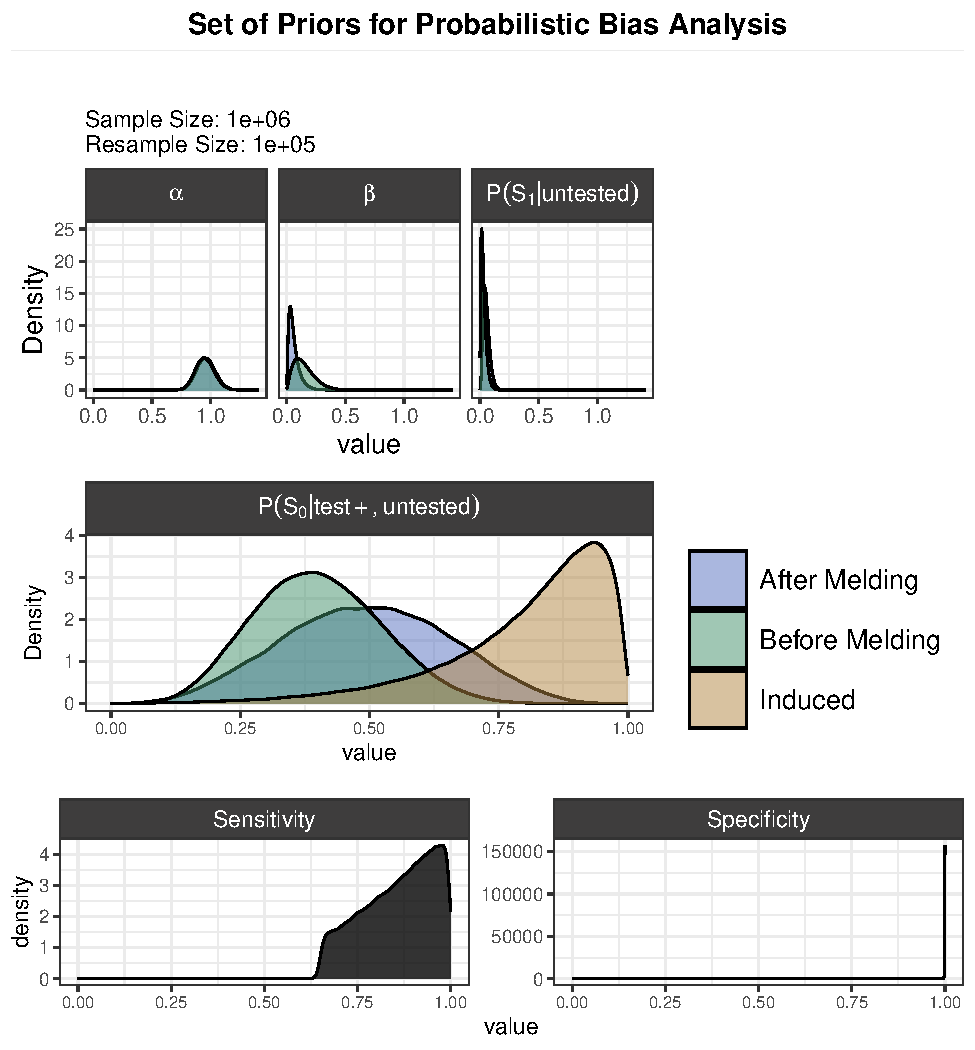
\includegraphics[width=0.5\linewidth]{thesis_files/figure-latex/unnamed-chunk-69-1} 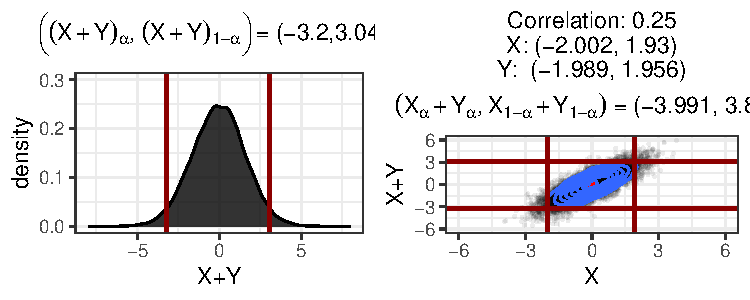
\includegraphics[width=0.5\linewidth]{thesis_files/figure-latex/unnamed-chunk-69-2} \caption{\label{fig:correctedsuffolk}}\label{fig:unnamed-chunk-69}
\end{figure}
\hypertarget{version-2-4-allowing-some-prior-parameters-to-vary}{%
\section{Version 2-4: Allowing Some Prior Parameters to Vary}\label{version-2-4-allowing-some-prior-parameters-to-vary}}

The implementation for versions 2-4 when considering a single time and geographic unit are almost identical to version 1; the difference is in the source of the priors.

For one version, we allow \(\beta\) to vary by date and state by using the COVID-19 Trends and Impact Survey (Salomon et al., 2021b). Since \(\beta\) represents the ratio of \(\dfrac{P(\text{test}_+|\text{untested},S_0)}{P(\text{test}_+|\text{tested})}\), one way we can think about estimating this quantity empirically is as the screening test positivity over the overall test positivity. Since both these quantities are reported by the COVID-19 Trends and Impact Survey, we can center the distribution for \(\beta\) for a given location and time interval at this ratio, after performing LOESS smoothing. That is, we use the same standard deviation assumed in the first version, where we do not allow priors to vary by state or date, but we set the mean to be the empirical estimate of beta.

For another version, we allow \(P(S_1|\text{untested})\) to vary by date and state by centering the distribution for \(P(S_1|\text{untested})\) at the percentage of COVID-19-like illness reported by the COVID-19 Trends and Impact Survey, since this variable reflects the presents of symptoms related to COVID-19 among the general population.

Lastly, in one version we center both the distribution for \(P(S_1|\text{untested})\) and \(\beta\) at their empirical values.

While we recognize taking values of the survey may in itself introduce biases, in the United States, there is little alternative to inform the priors for \(\beta\) or \(P(S_1|untested)\), particularly at a fine geographic scale. Some countries, for example, the United Kingdom, conducted PCR tests and recorded symptoms for a random sample of the population to estimate community prevalence of COVID-19 (Riley et al., 2021). A study like this would be able to estimate the test positivity rate among the untested population directly (and the asymptomatic or symptomatic positivity rates as well) rather than defining random variables \(\alpha\) and \(\beta\) to correct the observed test positivity rate.

In this sense, looking at the empirical estimates of \(P(S_1|untested)\) and \(\beta\) using the COVID-19 Trends and Impact Survey can provide a useful baseline for plausible values these parameters can take on, and allows us to see how the bias-corrected estimates differ depending on the data used to inform the priors.

\hypertarget{res}{%
\chapter{Results}\label{res}}

\hypertarget{comparison-to-the-covidestim-model}{%
\section{Comparison to the Covidestim Model}\label{comparison-to-the-covidestim-model}}

\hypertarget{overview-2}{%
\subsection{Overview}\label{overview-2}}

One challenge in correcting for biases in general is that although we may have some information about the influence of possible biases, we do not have a ground truth for comparison. However, one approach to handle the fact that the true cases are unobserved is comparing our estimates to those from other approaches seeking to estimate a similar quantity. In particular, if other approaches make different assumptions and come to a similar result, this can give us more confidence in our estimates.

One notable project seeking to estimate the true infection burden at the county-level over time is the COVIDestim project. In this work, Chitwood et al.~proposed a mechanistic model that includes states for asymptomatic/pre-symptomatic infection, symptomatic but mild infection, severe COVID-19 presentations, and death. This approach also enables the estimation of \(R_t\), the number of secondary infections a single infected individual causes at time \(t\). This is a useful quantity to estimate, but is sensitive to reporting delays and changes in testing practices (Pitzer et al., 2021).

\hypertarget{the-covidestim-model}{%
\subsection{The Covidestim Model}\label{the-covidestim-model}}

Chitwood \emph{et al.} propose a Bayesian evidence synthesis model to correct for reporting delays and time varying case ascertainment testing rate in the estimation of incident infections and \(R_t\).

To estimate the expected cases and deaths at a particular point in time, the model uses a convolution of the time series of observed cases and deaths and reporting delay distributions that are specific to the health state categories. This enables the model to account for the fact that reporting delay is different For any health state, for example, asymptomatic, the individual can either transition to the next health state (symptomatic) or recover. Thus, with each transition between a defined health state, for example, asymptomatic, there is a probability of transitioning to the next health state (in this case, asymptomatic to symptomatic); the complement of this probability is the probability of recovery.

Each of these transitions is defined by a delay distribution. For example, the distribution for moving from asymptomatic to symptomatic represents the probability an individual moves to the symptomatic state at a point in time. The probabilities asymptomatic to symptomatic and symptomatic to severe are modeled as not varying with time. Meanwhile, the probability of transitioning from severe to death was defined to be higher in 2020 due to higher case fatalities early in the pandemic. The infection fatality rates, adjusted to be specific to a given state or county based on age distributions and the prevalence of risk factors for COVID-19, are used to inform the probability of moving from the severe category to the death category.

The change in daily infections from the previous day (i.e., the new infections) is calculated as a function of the estimated effective reproductive number \(R_t\) and the mean serial interval, where serial interval is the time from the onset of infection of a primary case to the time of onset of infection in the secondary case. \(R_t\) is estimated using a log-transformed cubic spline, under the assumption individuals can only be infected once.

They also defined a distribution for the delay to diagnosis, which was distinct by health state category to reflect differences in diagnosis delays that occur depending on the disease severity.
The probability of diagnosis among different health states was allowed to vary by time to reflect changing testing rates throughout the pandemic.

A separate distribution models the reporting delay to correct the total number of diagnoses on a given day for the fact that these diagnoses correspond to past infections.

The observed cases and death data for each state to the model were fitted using negative binomial likelihood functions.

\hypertarget{assumptions}{%
\subsection{Assumptions}\label{assumptions}}

This approach relies on infection fatality ratios and death counts to estimate the true case counts. Thus, it is sensitive to estimates of infection fatality rate, with higher infection fatality ratio estimates resulting in lower estimated infections. The infection fatality ratio is defined as the proportion of COVID-19 infections that lead to death, which means there is uncertainty in estimating both the numerator and the denominator of the ratio. The true cumulative incidence depends on the same uncertainties in estimating the true case burden at any point in time. Estimating the infection fatality ratio itself is a challenging task.

The COVIDestim model uses age-specific estimates of IFR produced by O'Driscoll et al. (2021). This group used national-level age-stratified, and when possible sex-stratified, COVID-19 death counts and cumulative infection estimates from seroprevalence studies. Of note, the estimates of infection fatality ratio are assumed to be constant over time, which may not be the case due to improving treatments (e.g., Paxlovid), different variants leading to less severe presentations, or changes in the demographics of individuals being infected. However, reliable estimates of infection fatality ratio that vary with time difficult to acquire; COVIDestim assumed a higher case fatality in 2020 given the novelty of the virus and consequent lack of available treatments.

\hypertarget{the-model}{%
\subsection{The Model}\label{the-model}}

Chitwood et al.~propose a Bayesian evidence synthesis model. To estimate the expected cases and deaths at a particular point in time, the model uses a convolution of the time series of observed cases and deaths and reporting delay distributions that are specific to the health state categories. This enables the model to account for the fact that reporting delay is different For any health state, for example, asymptomatic, the individual can either transition to the next health state (symptomatic) or recover. Thus, with each transition between a defined health state, for example, asymptomatic, there is a probability of transitioning to the next health state (in this case, asymptomatic → symptomatic); the complement of this probability is the probability of recovery.

Each of these transitions is defined by a delay distribution. For example, the distribution for moving from asymptomatic to symptomatic represents the probability an individual moves to the symptomatic state at a point in time. The probabilities asymptomatic to symptomatic and symptomatic to severe are modeled as not varying with time. Meanwhile, the probability of transitioning from severe to death was defined to be higher in 2020 due to higher case fatalities early in the pandemic. The infection fatality rates, adjusted to be specific to a given state or county based on age distributions and the prevalence of risk factors for COVID-19, are used to inform the probability of moving from the severe category to the death category.

The change in daily infections from the previous day (i.e., the new infections) is calculated as a function of the estimated effective reproductive number \(R_t\) and the mean serial interval, where serial interval is the time from the onset of infection of a primary case to the time of onset of infection in the secondary case. \(R_t\) is estimated using a log-transformed cubic spline, under the assumption individuals can only be infected once.

They also defined a distribution for the delay to diagnosis, which was distinct by health state category to reflect differences in diagnosis delays that occur depending on the disease severity.
The probability of diagnosis among different health states was allowed to vary by time to reflect changing testing rates throughout the pandemic.

A separate distribution models the reporting delay to correct the total number of diagnoses on a given day for the fact that these diagnoses correspond to past infections.

The observed cases and death data for each state to the model were fitted using negative binomial likelihood functions.

\hypertarget{comparison-to-serological-data}{%
\subsection{Comparison to Serological Data}\label{comparison-to-serological-data}}

There are known issues with seroprevalence estimates. For one, these samples are drawn from a convenience (i.e.~nonrandom) sample of individuals with blood specimens taken for purposes other than COVID-19 antibody detection ({``Commercial {Laboratory Seroprevalence Surveys} \textbar{} {Coronavirus} \textbar{} {COVID-19} \textbar{} {CDC},''} n.d.). Secondly, while a positive serological test is evidence for infection, a negative serological test is less clear to interpret. The person may have been infected but not yet have developed antibodies, or their immune system may not have produced antibodies at a detectable level {[}CDC (2020).

Indeed, Chitwood et al.~found limited concordance between their estimates and seroprevalence data. However, there was a stronger correlation between estimates of cumulative infection and cumulative hospitalizations and cumulative deaths \footnote{The correlation employed here is the Spearman rank correlation, which measures the strength of the monotonic relationship rather than the strength of the linear relationship, in which case the Pearson correlation coefficient is the usual choice. The Spearman rank correlation is equivalent to the Pearson correlation of the rank values rather than the values themselves. }.

\hypertarget{lims}{%
\subsection{Limitations of this Comparison}\label{lims}}

At this point in the pandemic, there is no true gold standard to compare to. Covidestim is one model, among many, that makes key assumptions about aspects of the virus. Another note is that estimates from the Covidestim model are reported on the daily timescale for counties, while the probabilistic approach we implemented here is at the biweekly time scale.

To ensure the comparisons are on the same time scale, we sum the reported 95\% credible intervals for the days in each 2-week interval. These intervals do not represent a 95\% credible interval for the 2-week interval, and while such an interval would be ideal for the comparison, computation of a 95\% credible interval for the two-week interval is not feasible because of the model structure. Due to the correlation between observations for each day for a given location, summing the intervals yields an estimate that is likely to be more conservative than a true 95\% credible interval for the two-week interval would be. More detail on this assumption is in \protect\hyperlink{conservativeintervals}{the appendix}.

\hypertarget{county-level-results}{%
\section{County-level Results}\label{county-level-results}}

We performed county-level probabilistic bias analysis for Michigan and Massachusetts. This work can be expanded to consider other states as well where the needed data is available. In particular, we need both county-level positive PCR tests and county-level total PCR tests. Because the assumptions of the bias correction are related to test positivity, it does not make sense to apply the method to a positive cases count that includes positive PCR tests lumped together with probable cases. In some states, this is the only value reported.

\hypertarget{massachusetts}{%
\subsection{Massachusetts}\label{massachusetts}}

Figure \ref{fig:pb_counts_ma} shows the bias corrected estimates for each implementation, as well as the observed cases. We note that the lower bounds of the bias corrected estimates are always above the observed cases because adding (unobserved) infections among the untested population to the observed positives among the population never results in a decrease in the estimated infections. In theory such a decrease could be possible since we do correct for differences due to imperfect test accuracy, and if the false positive rate was high enough, we might estimate the lower bound of cases as lower than the observed cases. However, the false positive rate of the COVID-19 PCR test is so low that in practice we do not see lower bounds lower than the number of infections.\footnote{The false positive rate differs by platform and laboratory, but multiple analyses estimated that it is less than 0.10\% (Chandler, Bourassa, Mathias, \& Greninger, 2021).}

We can see although the trends are broadly similar between versions for each county, centering the distribution at the empirical value of \(\beta\) leads to peaks not present in the version where priors do not vary by county and date. However, only centering \(P(S_1|\text{untested})\) at the empirical value leads to a distribution that is highly similar to the version where priors do not vary by county and date.

These results make sense when we consider that this analysis is much more sensitive to the choice of \(\beta\) than \(P(S_1|\text{untested})\). This follows from the fact we compute the number of positive infections among those who are untested and \emph{asymptomatic} as
\begin{align*}
N^+_{untested,S_0} &= P(\text{test}_+| S_0,\text{untested}) (N_{S_0,\text{untested}})\\
&= \Big( \beta P(test_+ |tested) \Big) N_{\text{untested}} (1-P(S_1|\text{untested}))
\end{align*}
and the number of positive infections among those who are untested and \emph{symptomatic} as\\
\begin{align*} N^+_{\text{untested},S_1}& = P(\text{test}_+| S_1,\text{untested}) (N_{S_1,\text{untested}})\\
&= \Big( \alpha P(\text{test}_+ |\text{tested}) \Big) N_{\text{untested}} (P(S_1|\text{untested})).
\end{align*}
Since \(N_{S_1, \text{untested}}\) is so much larger than \(N_{S_1, \text{untested}}\) for any of the specified values of \(P(S_1|\text{untested})\) (since the bulk of this distribution is less than 5\%), \(\beta\) has a larger impact on the number of estimated infections.
\begin{figure}
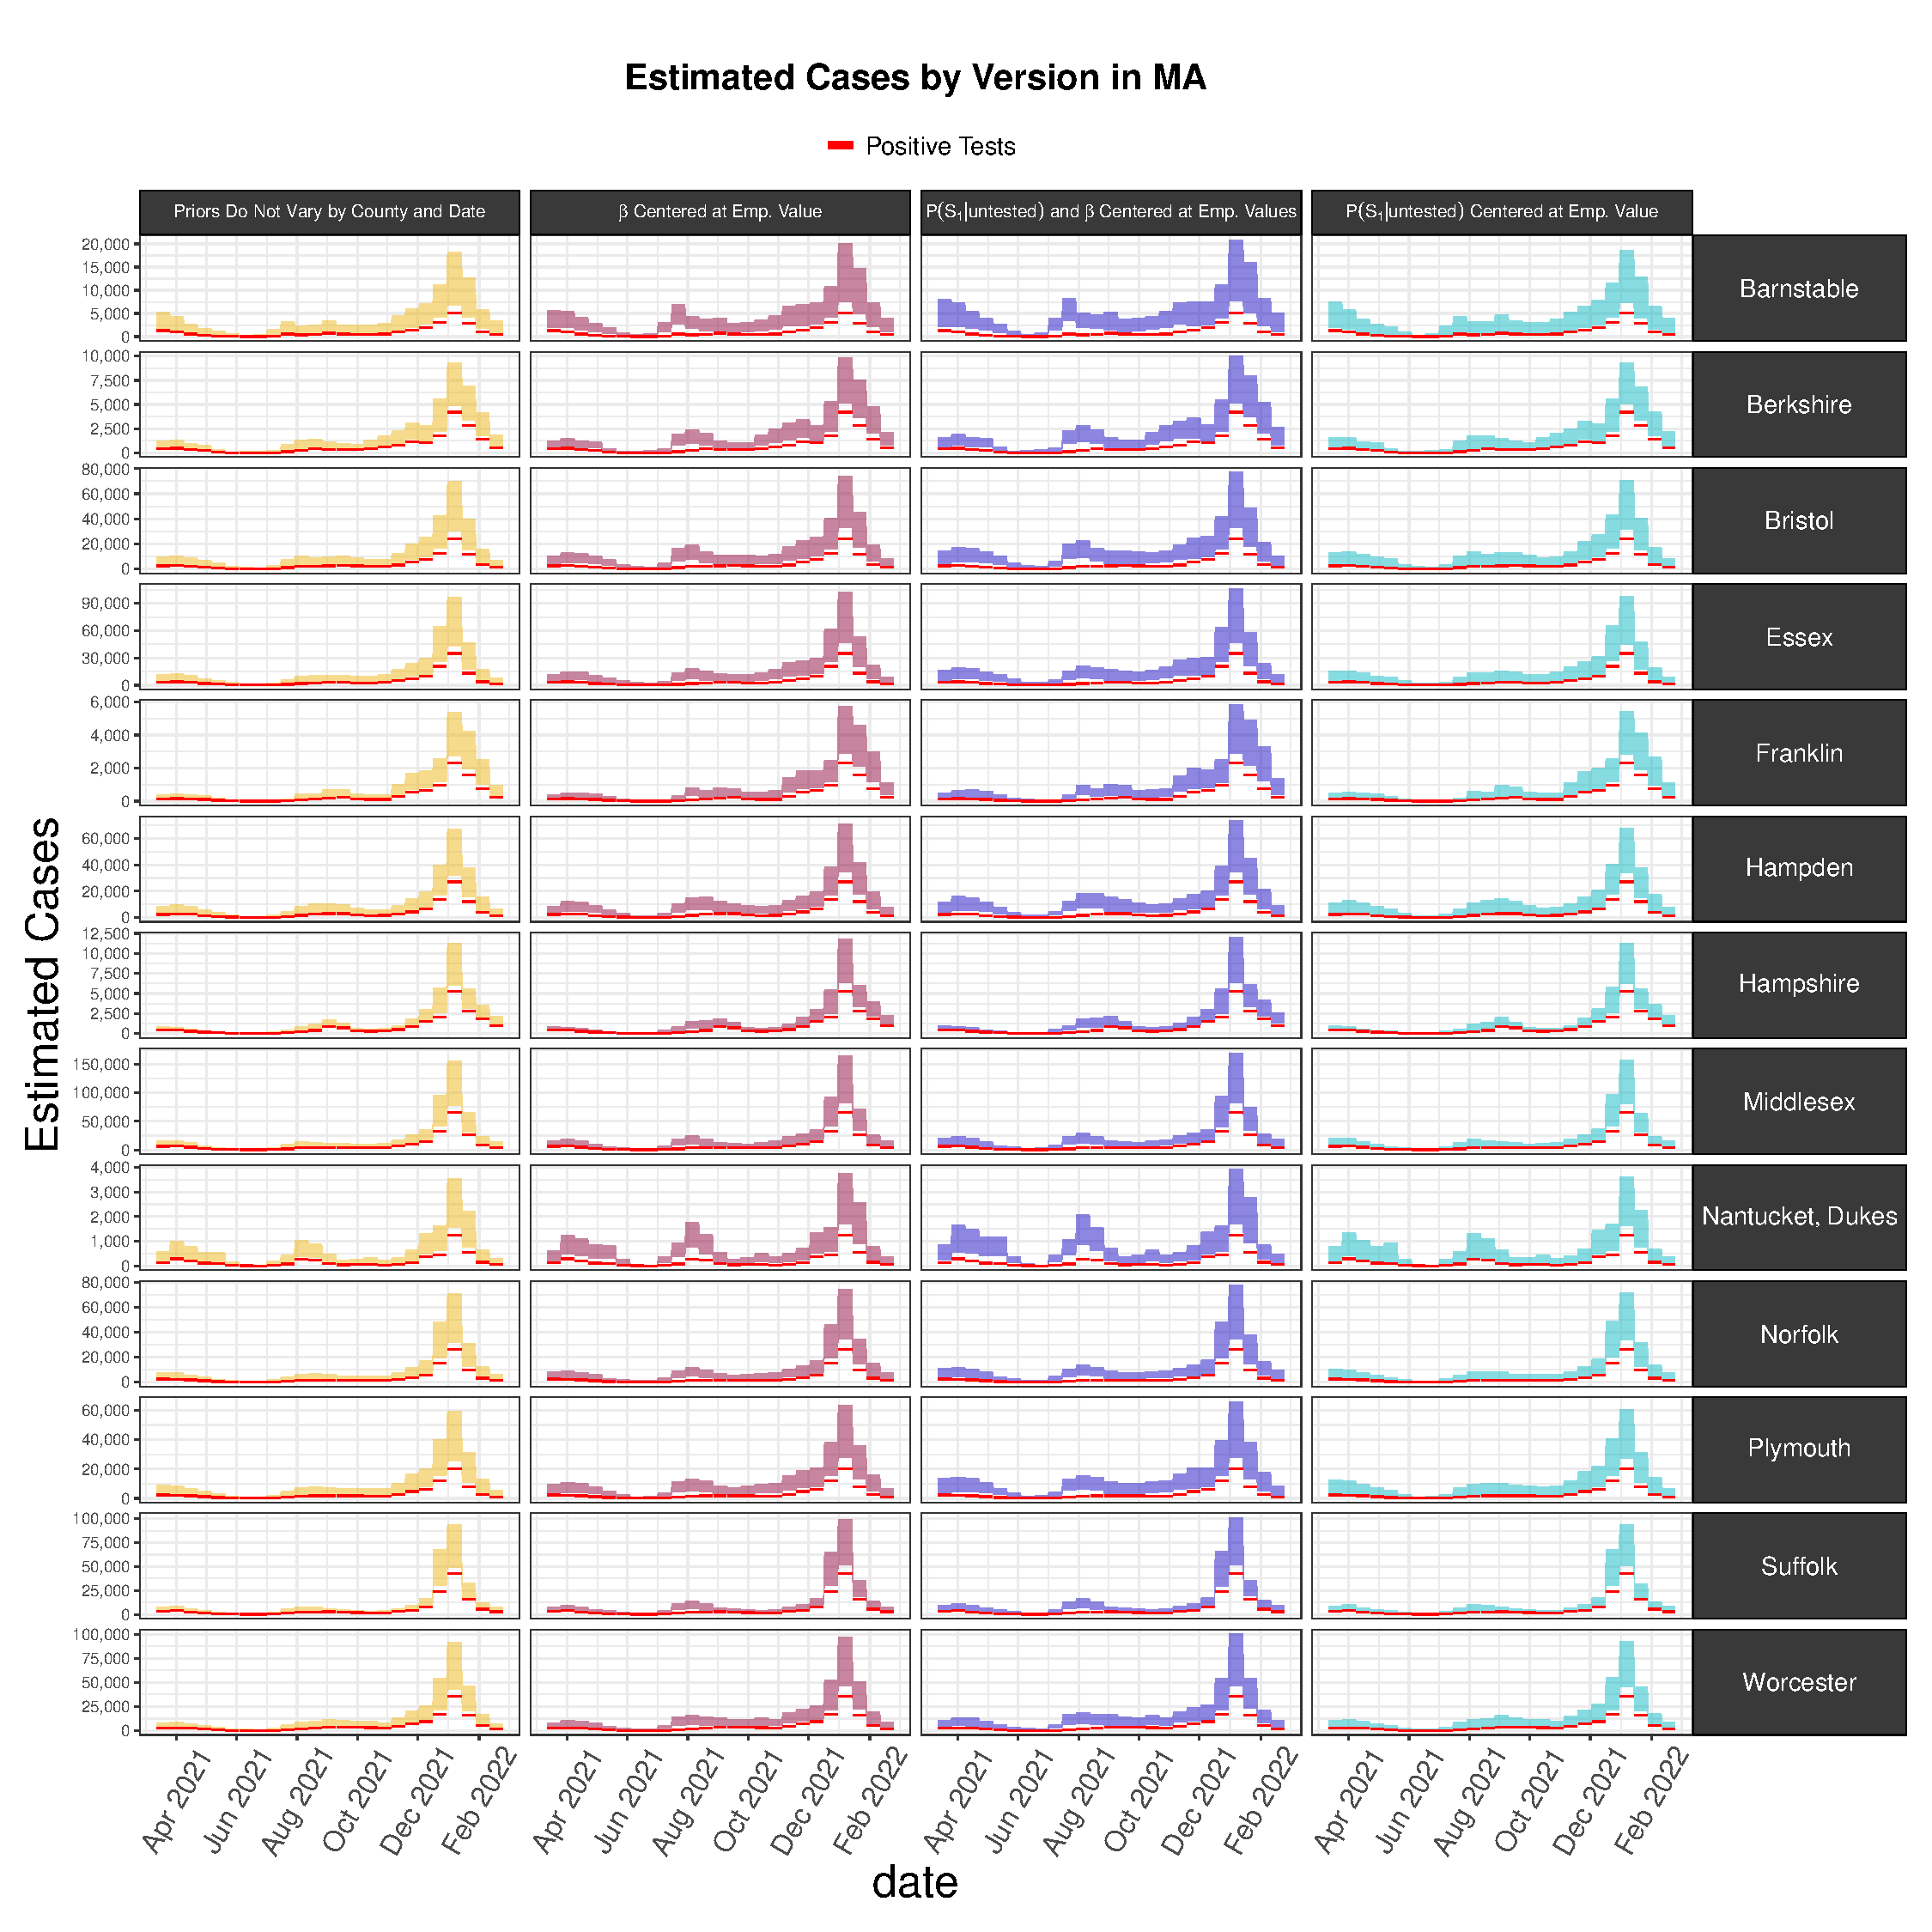
\includegraphics[width=0.95\linewidth]{figure/ma_pb_compared_to_observed} \caption{\label{fig:pb_counts_ma}}\label{fig:unnamed-chunk-71}
\end{figure}
To better see the overlap between versions, in Figure \ref{fig:pb_versions_ma} we can look at the versions together. This allows us to see more clearly how the version with both \(P(S_1|\text{untested})\) and \(\beta\) centered at their empirical values is consistently the highest. Meanwhile, the version with only \(P(S_1|untested)\) centered at its empirical value corresponds so closely to the version that does not vary by date or location that there is no part of the intervals for the version not varying by date or location that do not overlap with the \(P(S_1|\text{untested})\) version.
\begin{figure}
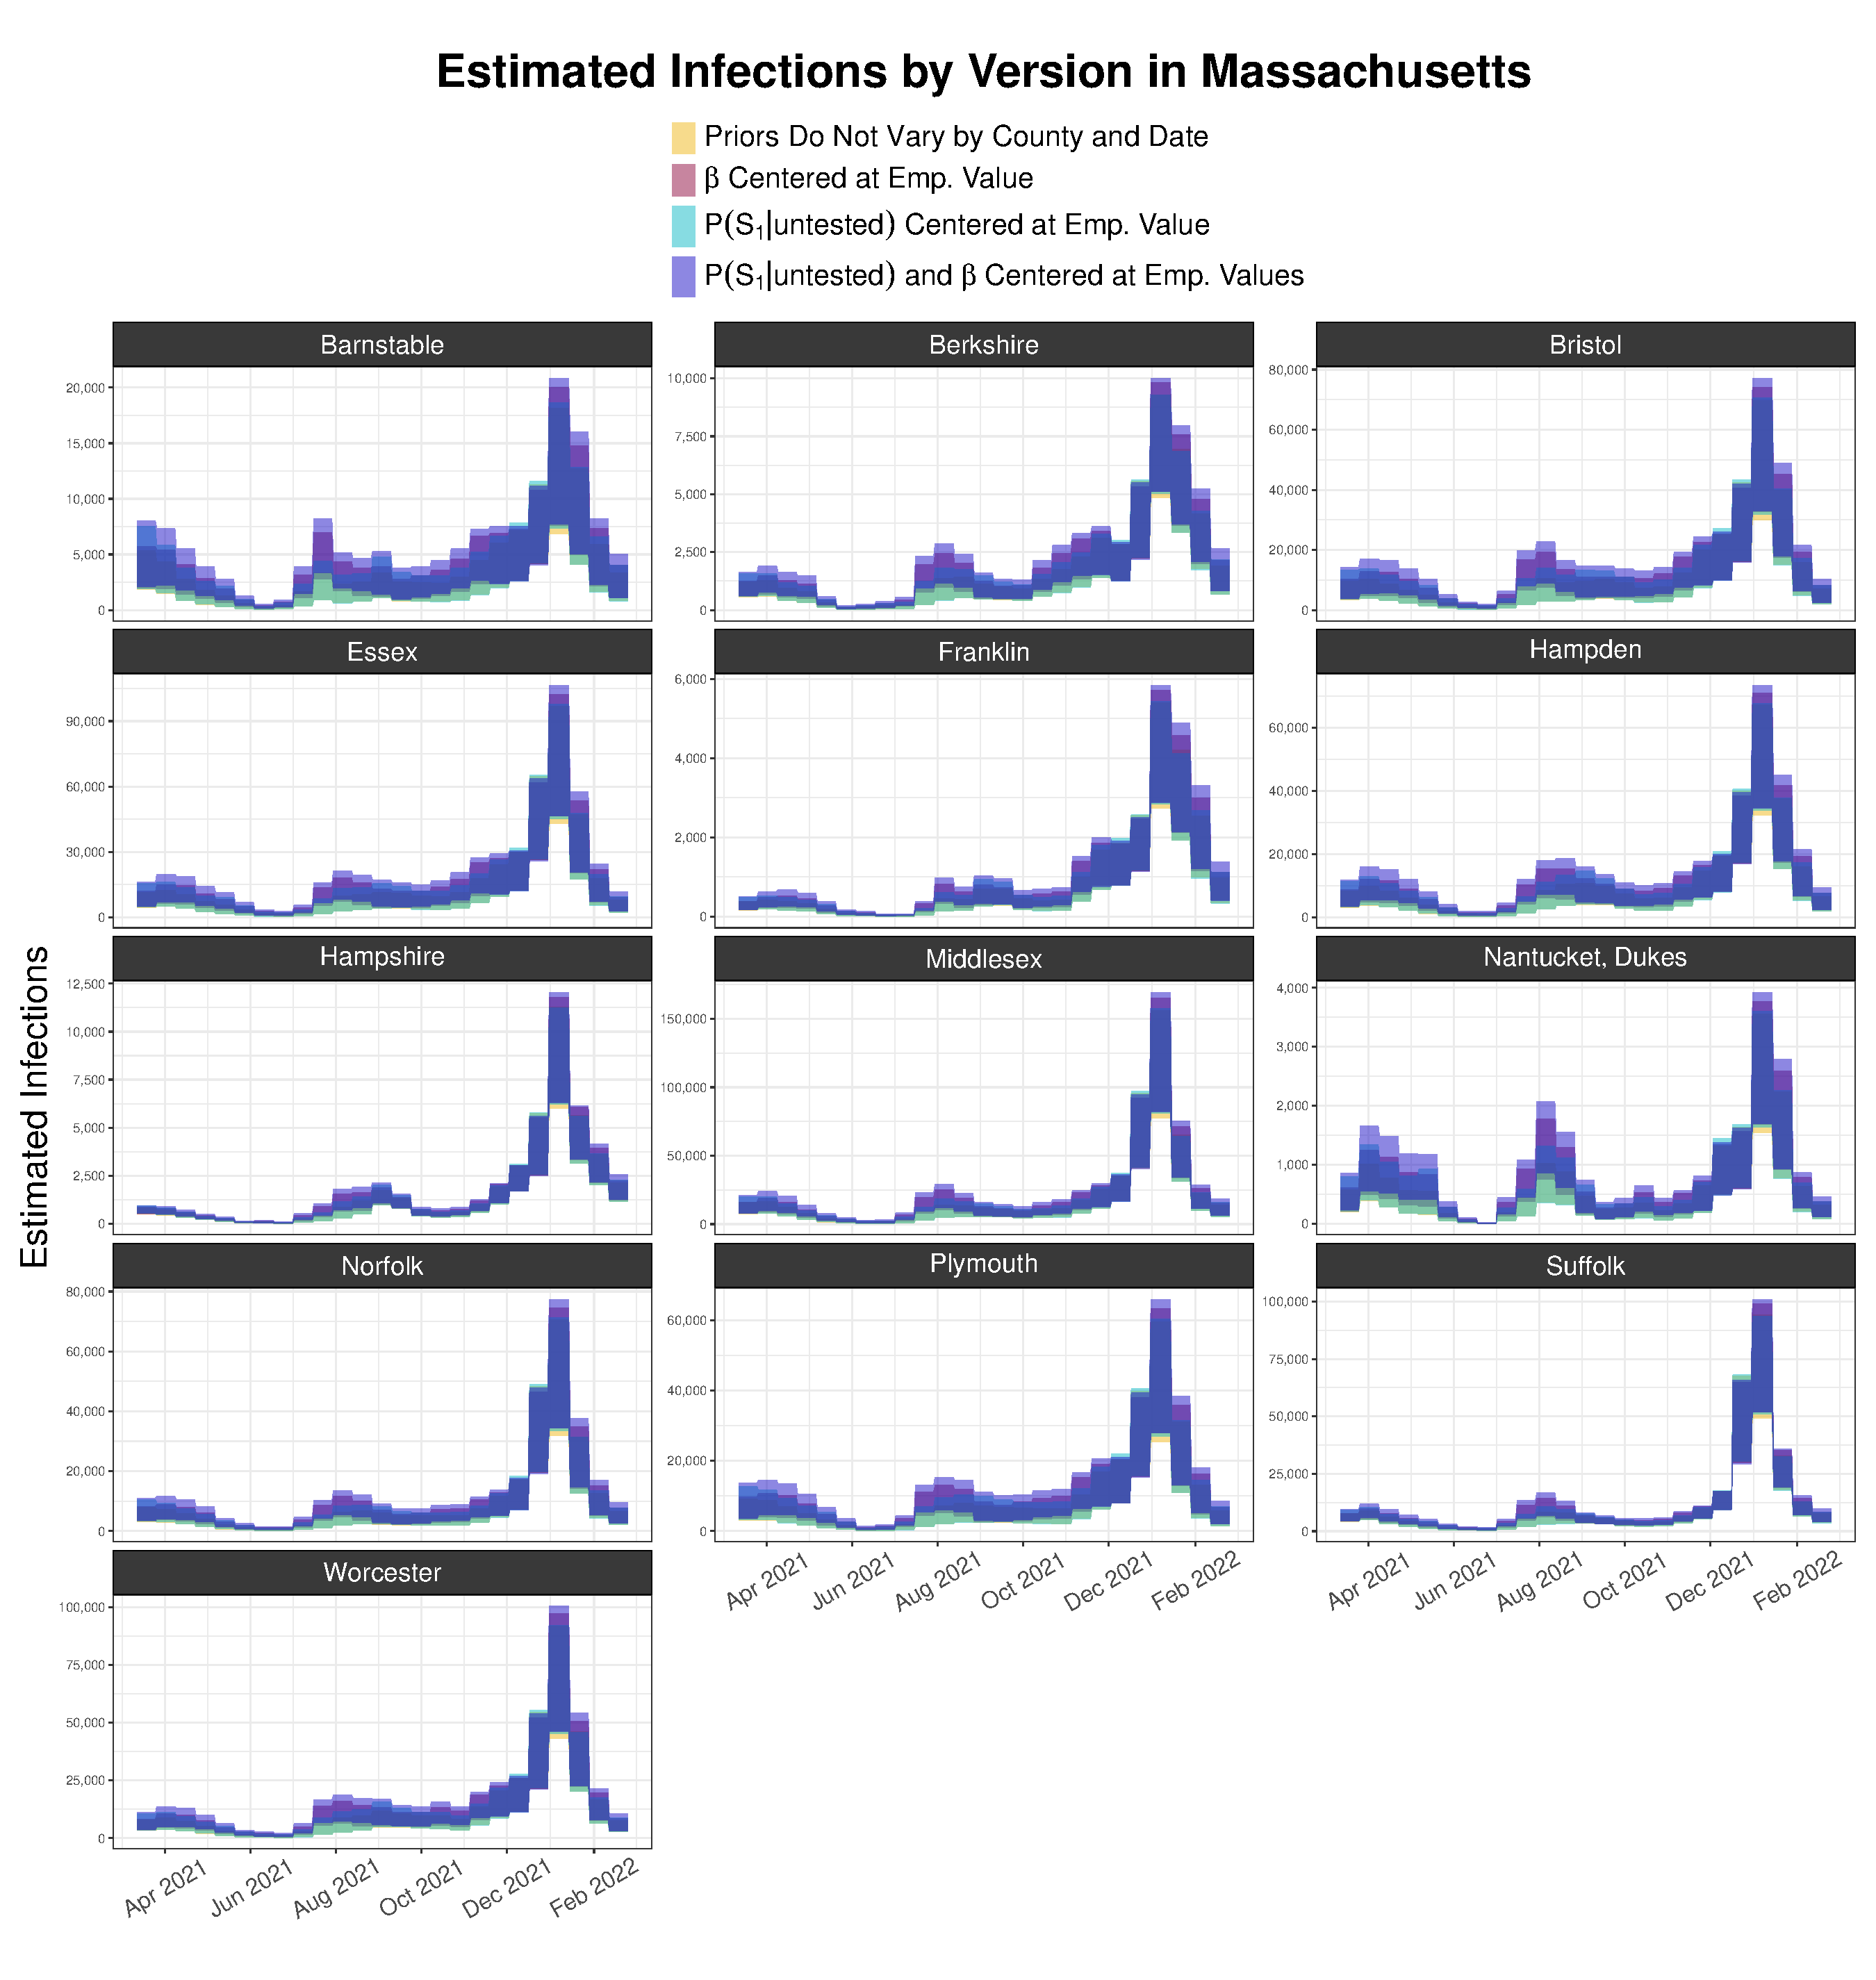
\includegraphics[width=0.95\linewidth]{figure/ma_pb_compare_versions} \caption{\label{fig:pb_versions_ma}}\label{fig:unnamed-chunk-72}
\end{figure}
Now, we can also compare the extent to which these intervals agree with the Covidestim estimates. In \ref{fig:pb_covidestim_ma}, we see that when Covidestim estimates fall outside the probabilistic bias intervals, they fall below the intervals, estimating that there are less infections. The exception here is Hampshire County, which actually is very likely to be related to the high amount of asymptomatic testing done among the five colleges. Smith College alone, with a student body of about 2,500 and mandatory PCR testing twice a week, would contribute a substantial amount of tests to the test count in Hampshire County. Given the low infection burden, the vast majority of these tests were negative throughout most of 2021, reducing the positivity rate (Figure \ref{fig:hamp}). The extensive amount of asymptomatic testing done here would mean that
means that our correction factor \(\beta\) in probabilistic analysis\footnote{Recall \(P(\text{test}_+ | S_0, \text{untested}) = \beta \; P(\text{test}_+|\text{tested})\).}, which we use to estimate the positivity rate among the untested asymptomatic population, would be too low. This is because the observed test positivity rate when so much asymptomatic testing is conducted would be closer to what expect the positivity rate among the asymptomatic test positivity rate to be among the untested population. Because the assumptions of the probabilistic bias analysis here did not assume such extensive asymptomatic testing was contributing to the test positivity rate, we are likely underestimating the true number of unobserved infections if there is a substantial amount of screening testing. It would be simple, however, to adjust \(\beta\) to account for cases where there is increased asymptomatic testing.
\begin{figure}
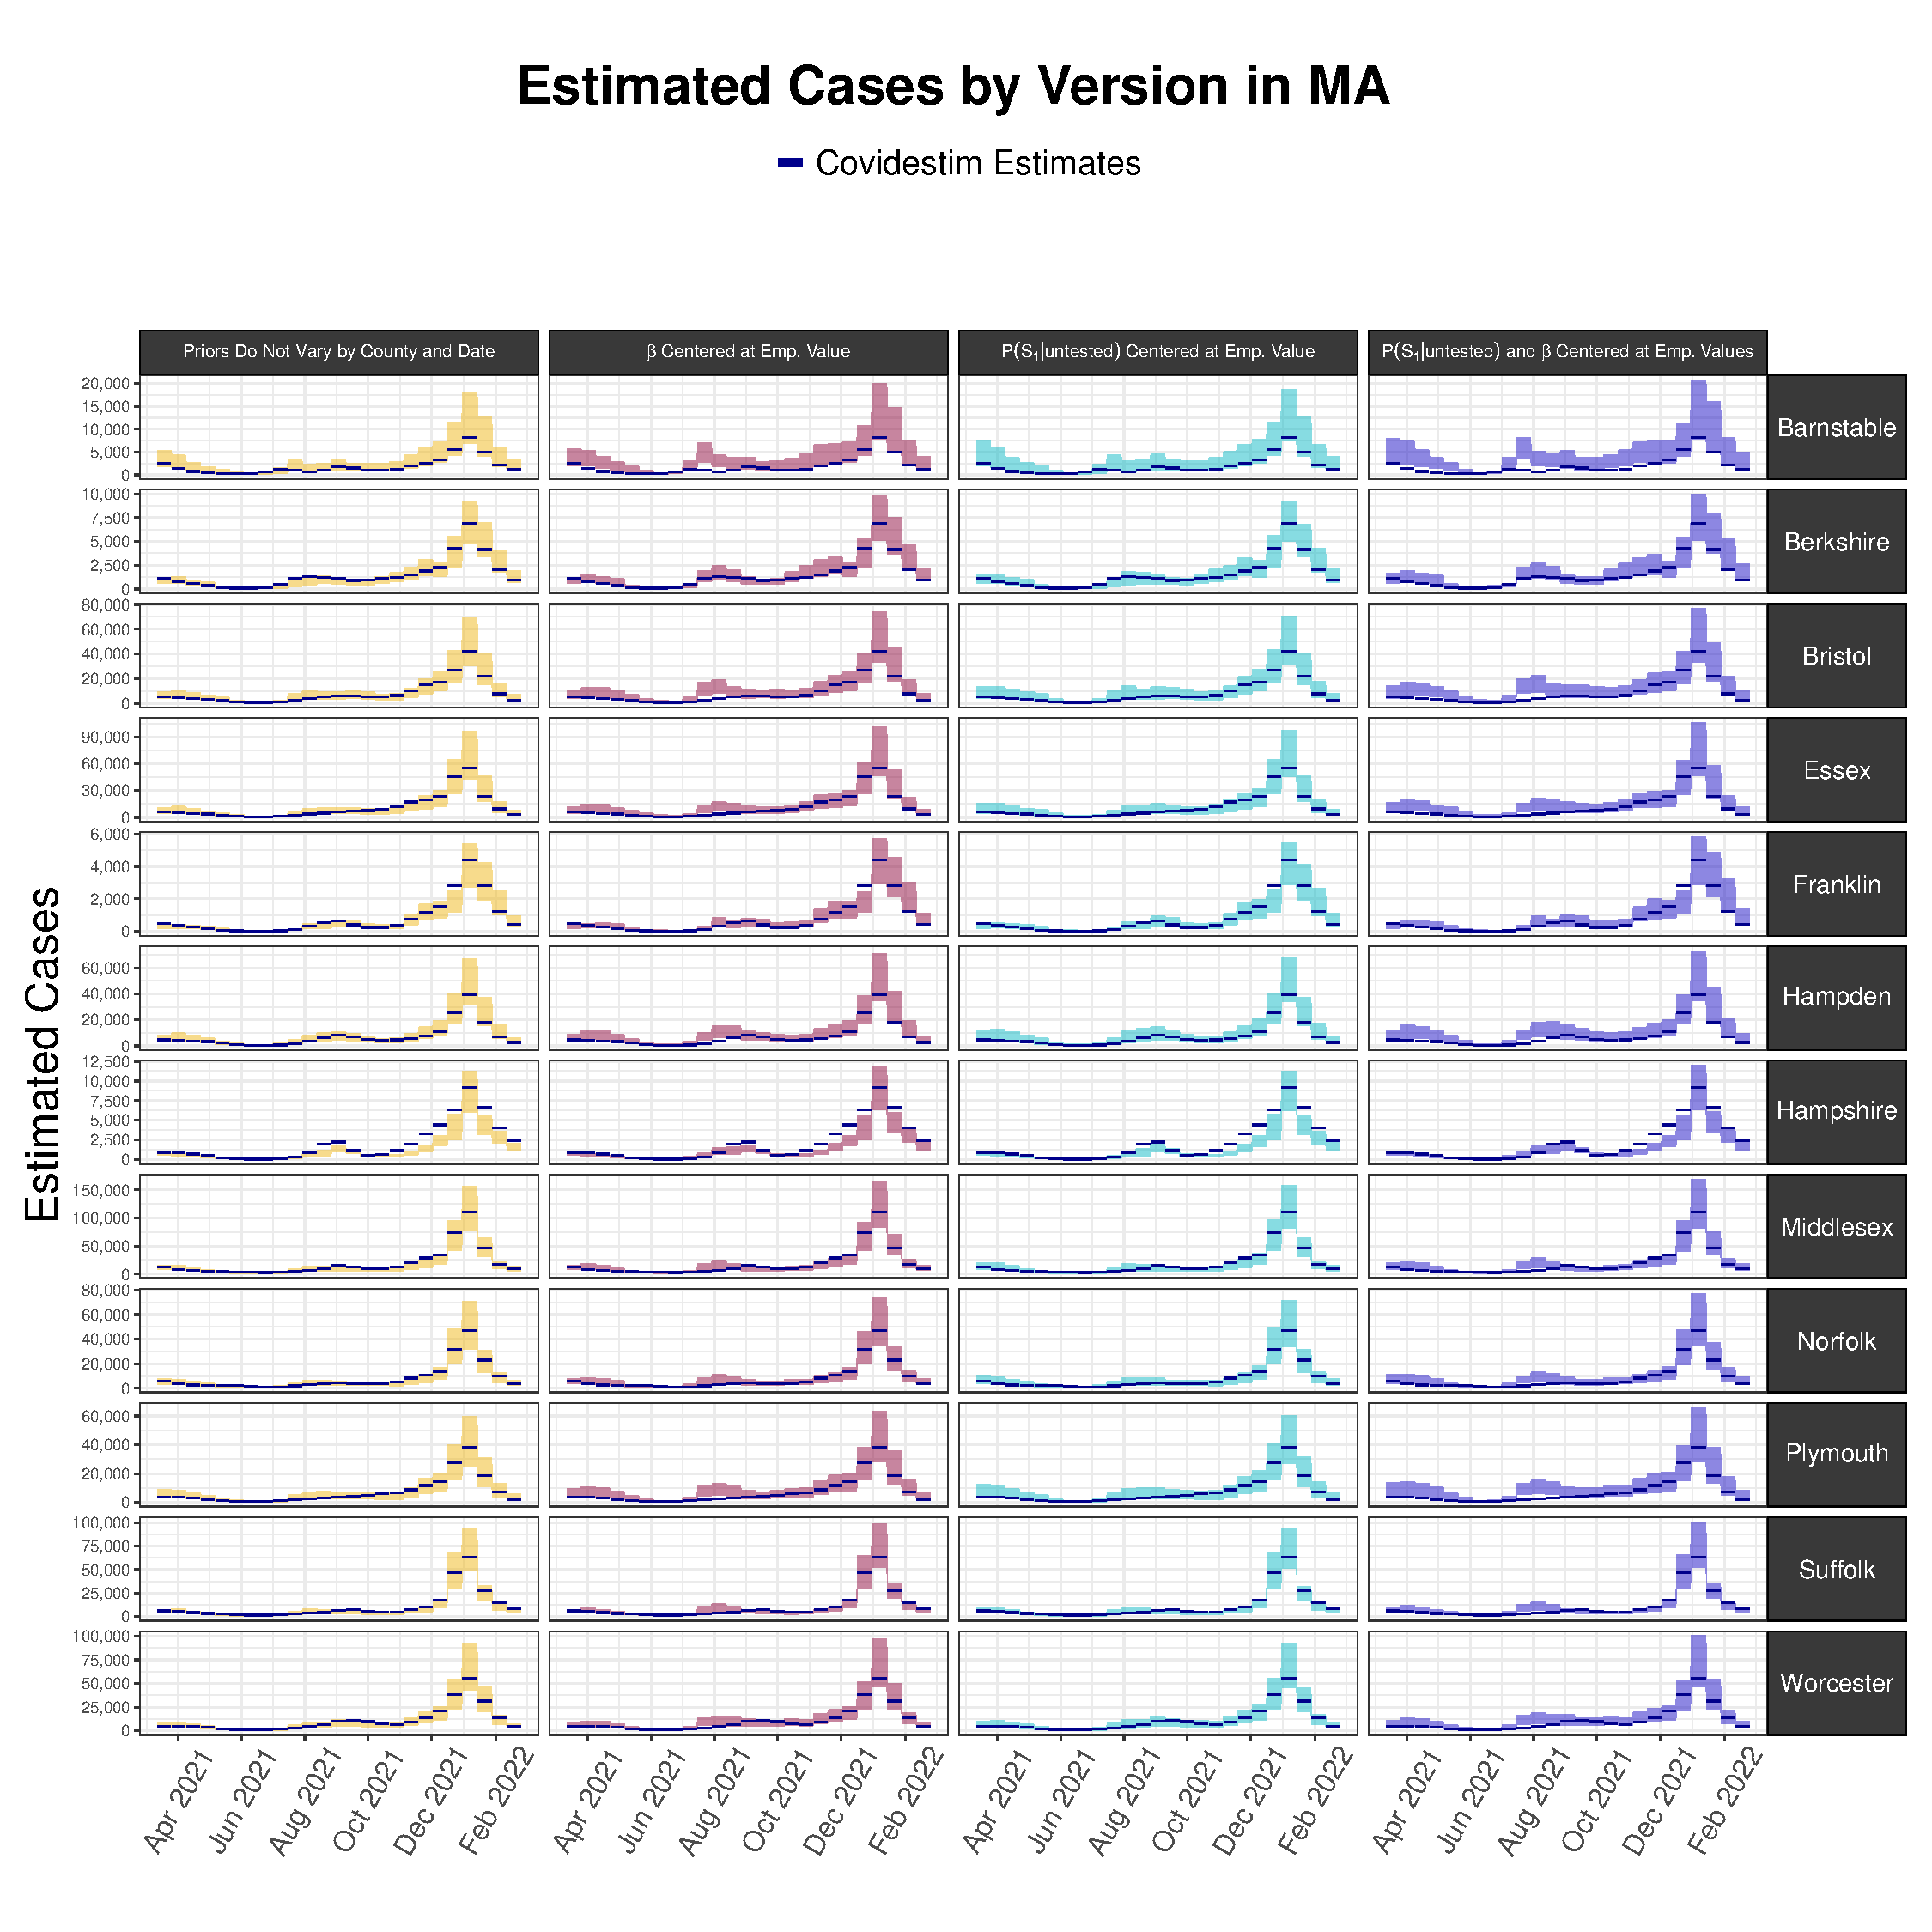
\includegraphics[width=1\linewidth]{figure/ma_pb_compared_to_covidestim} \caption{\label{fig:pb_covidestim_ma}}\label{fig:unnamed-chunk-73}
\end{figure}
\begin{figure}
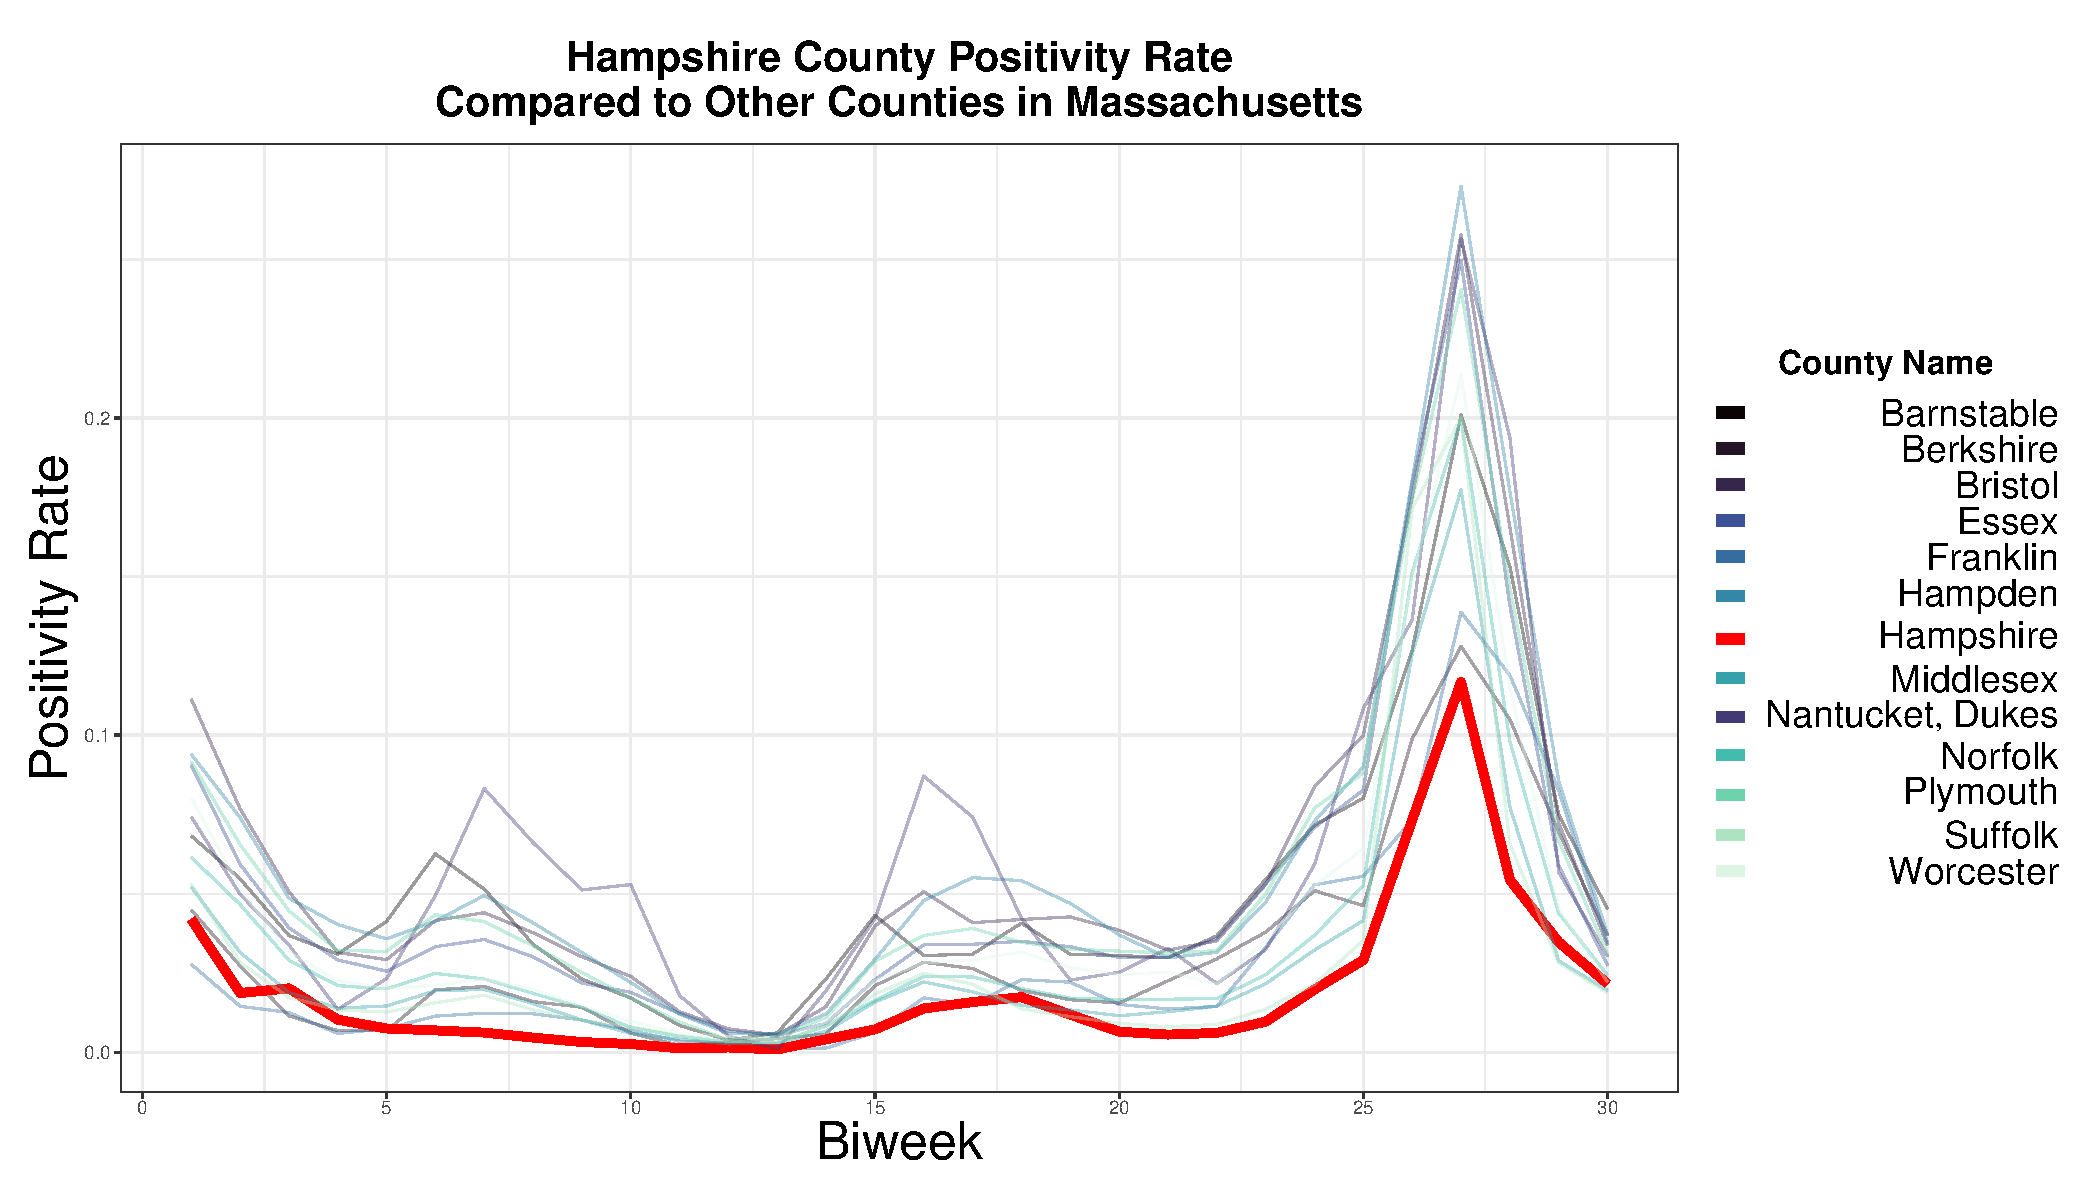
\includegraphics[width=0.9\linewidth]{figure/hampshire} \caption{\label{fig:hamp} We see that Hampshire County has among the lowest test positivity rates among counties in Massachusetts in the time period considered.}\label{fig:unnamed-chunk-74}
\end{figure}
To summarize which versions are most concordant with the Covidestim estimates, we can consider the proportion of the biweeks where the interval contains the Covidestim estimate. As we see in Figure \ref{fig:covidestimprop}, the implementation with the prior for \(P(S_1|\text{untested})\) centered at the empirical value tends to agree most with the Covidestim estimates.
\begin{figure}
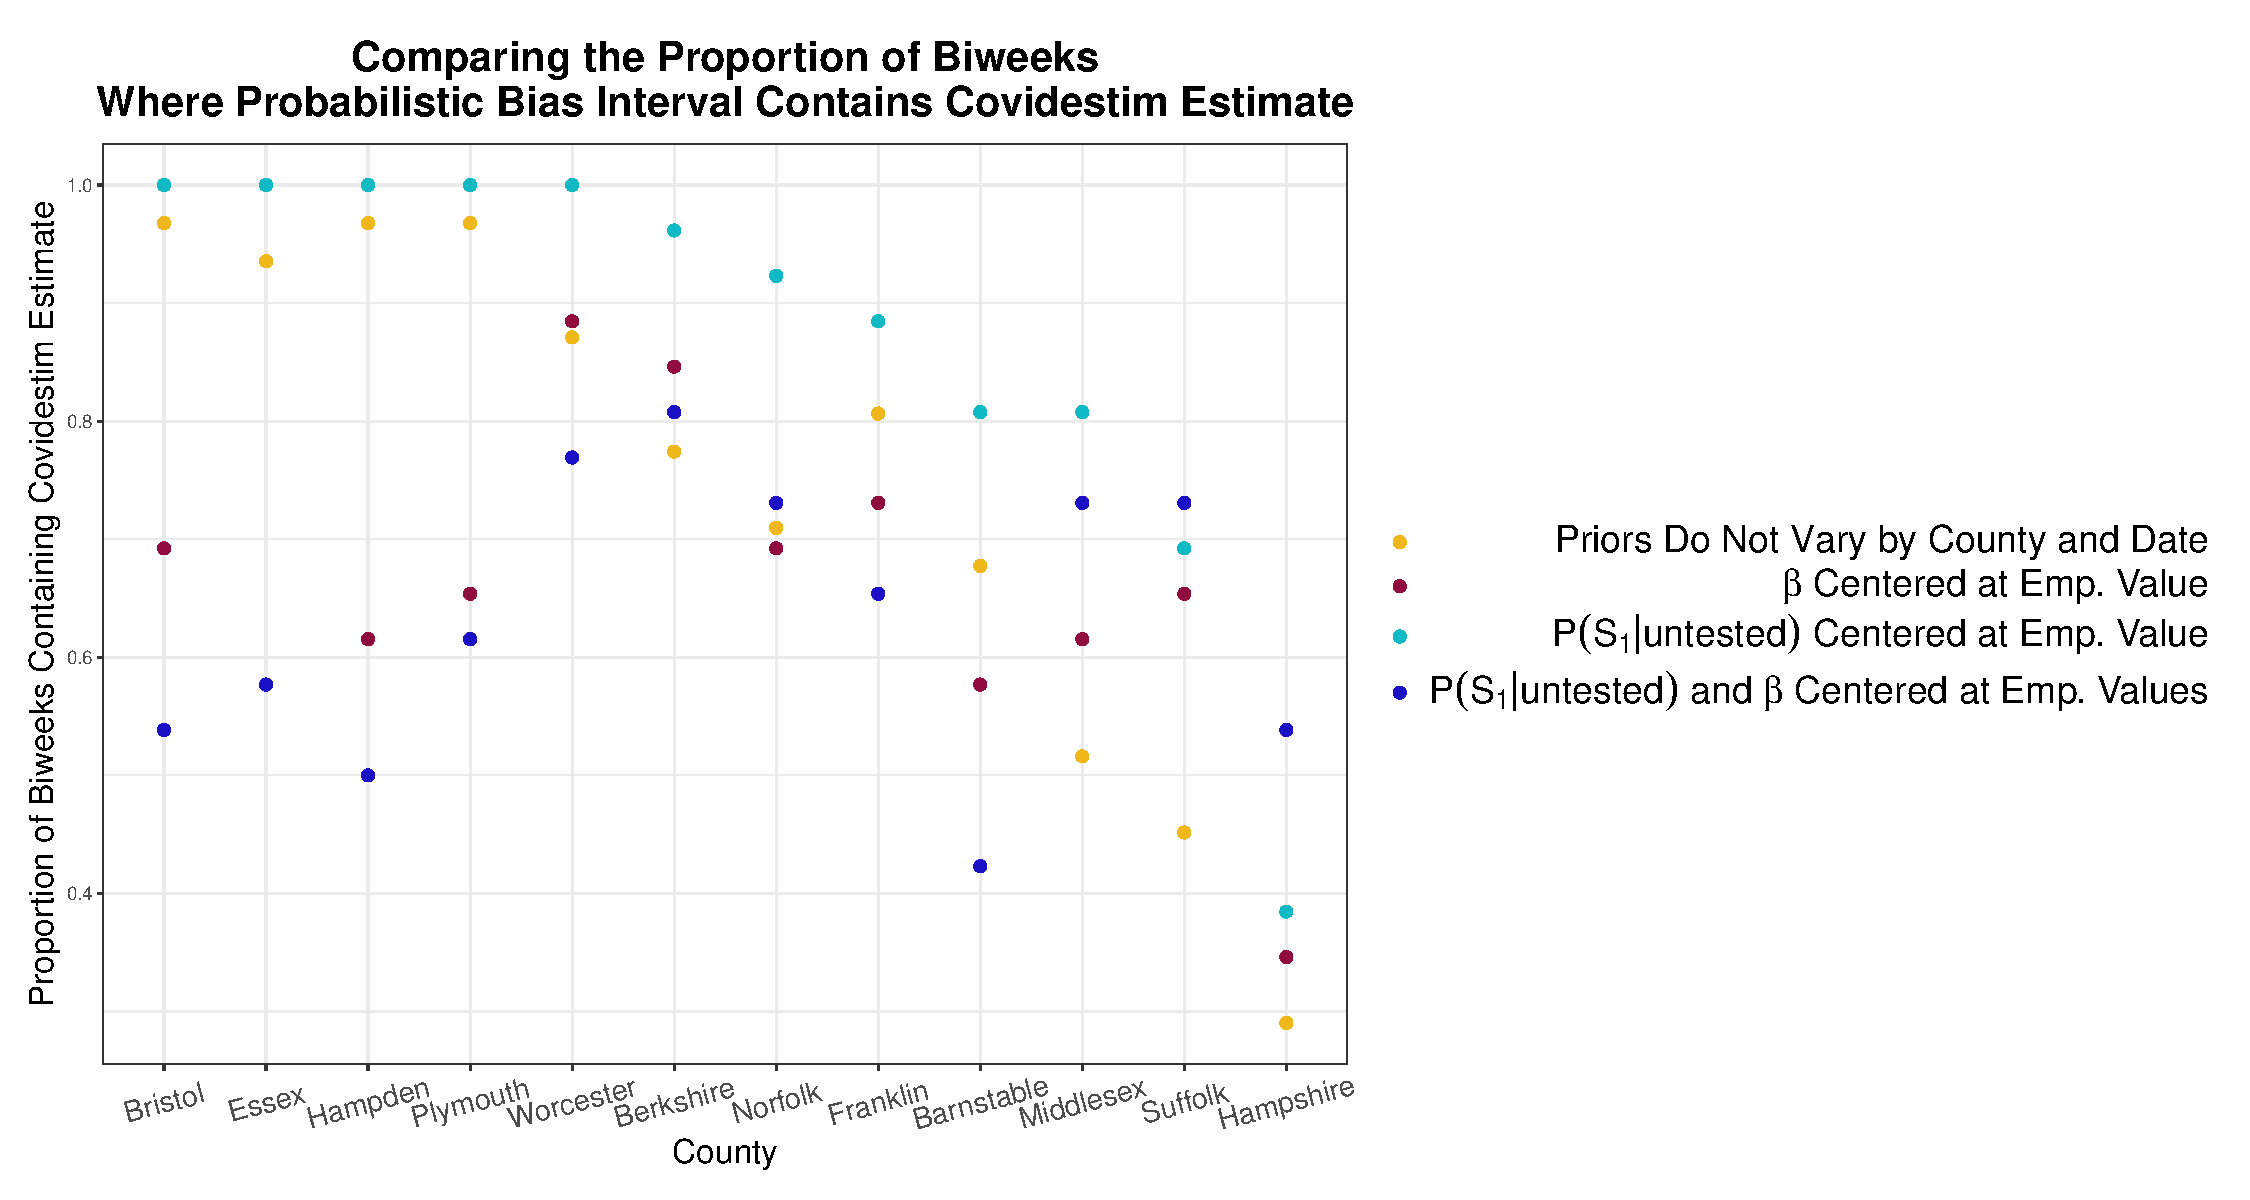
\includegraphics[width=1\linewidth]{figure/ma_pb_compared_to_covidestim_proportions} \caption{\label{fig:covidestimprop}}\label{fig:unnamed-chunk-75}
\end{figure}
\hypertarget{michigan}{%
\subsection{Michigan}\label{michigan}}
\begin{figure}
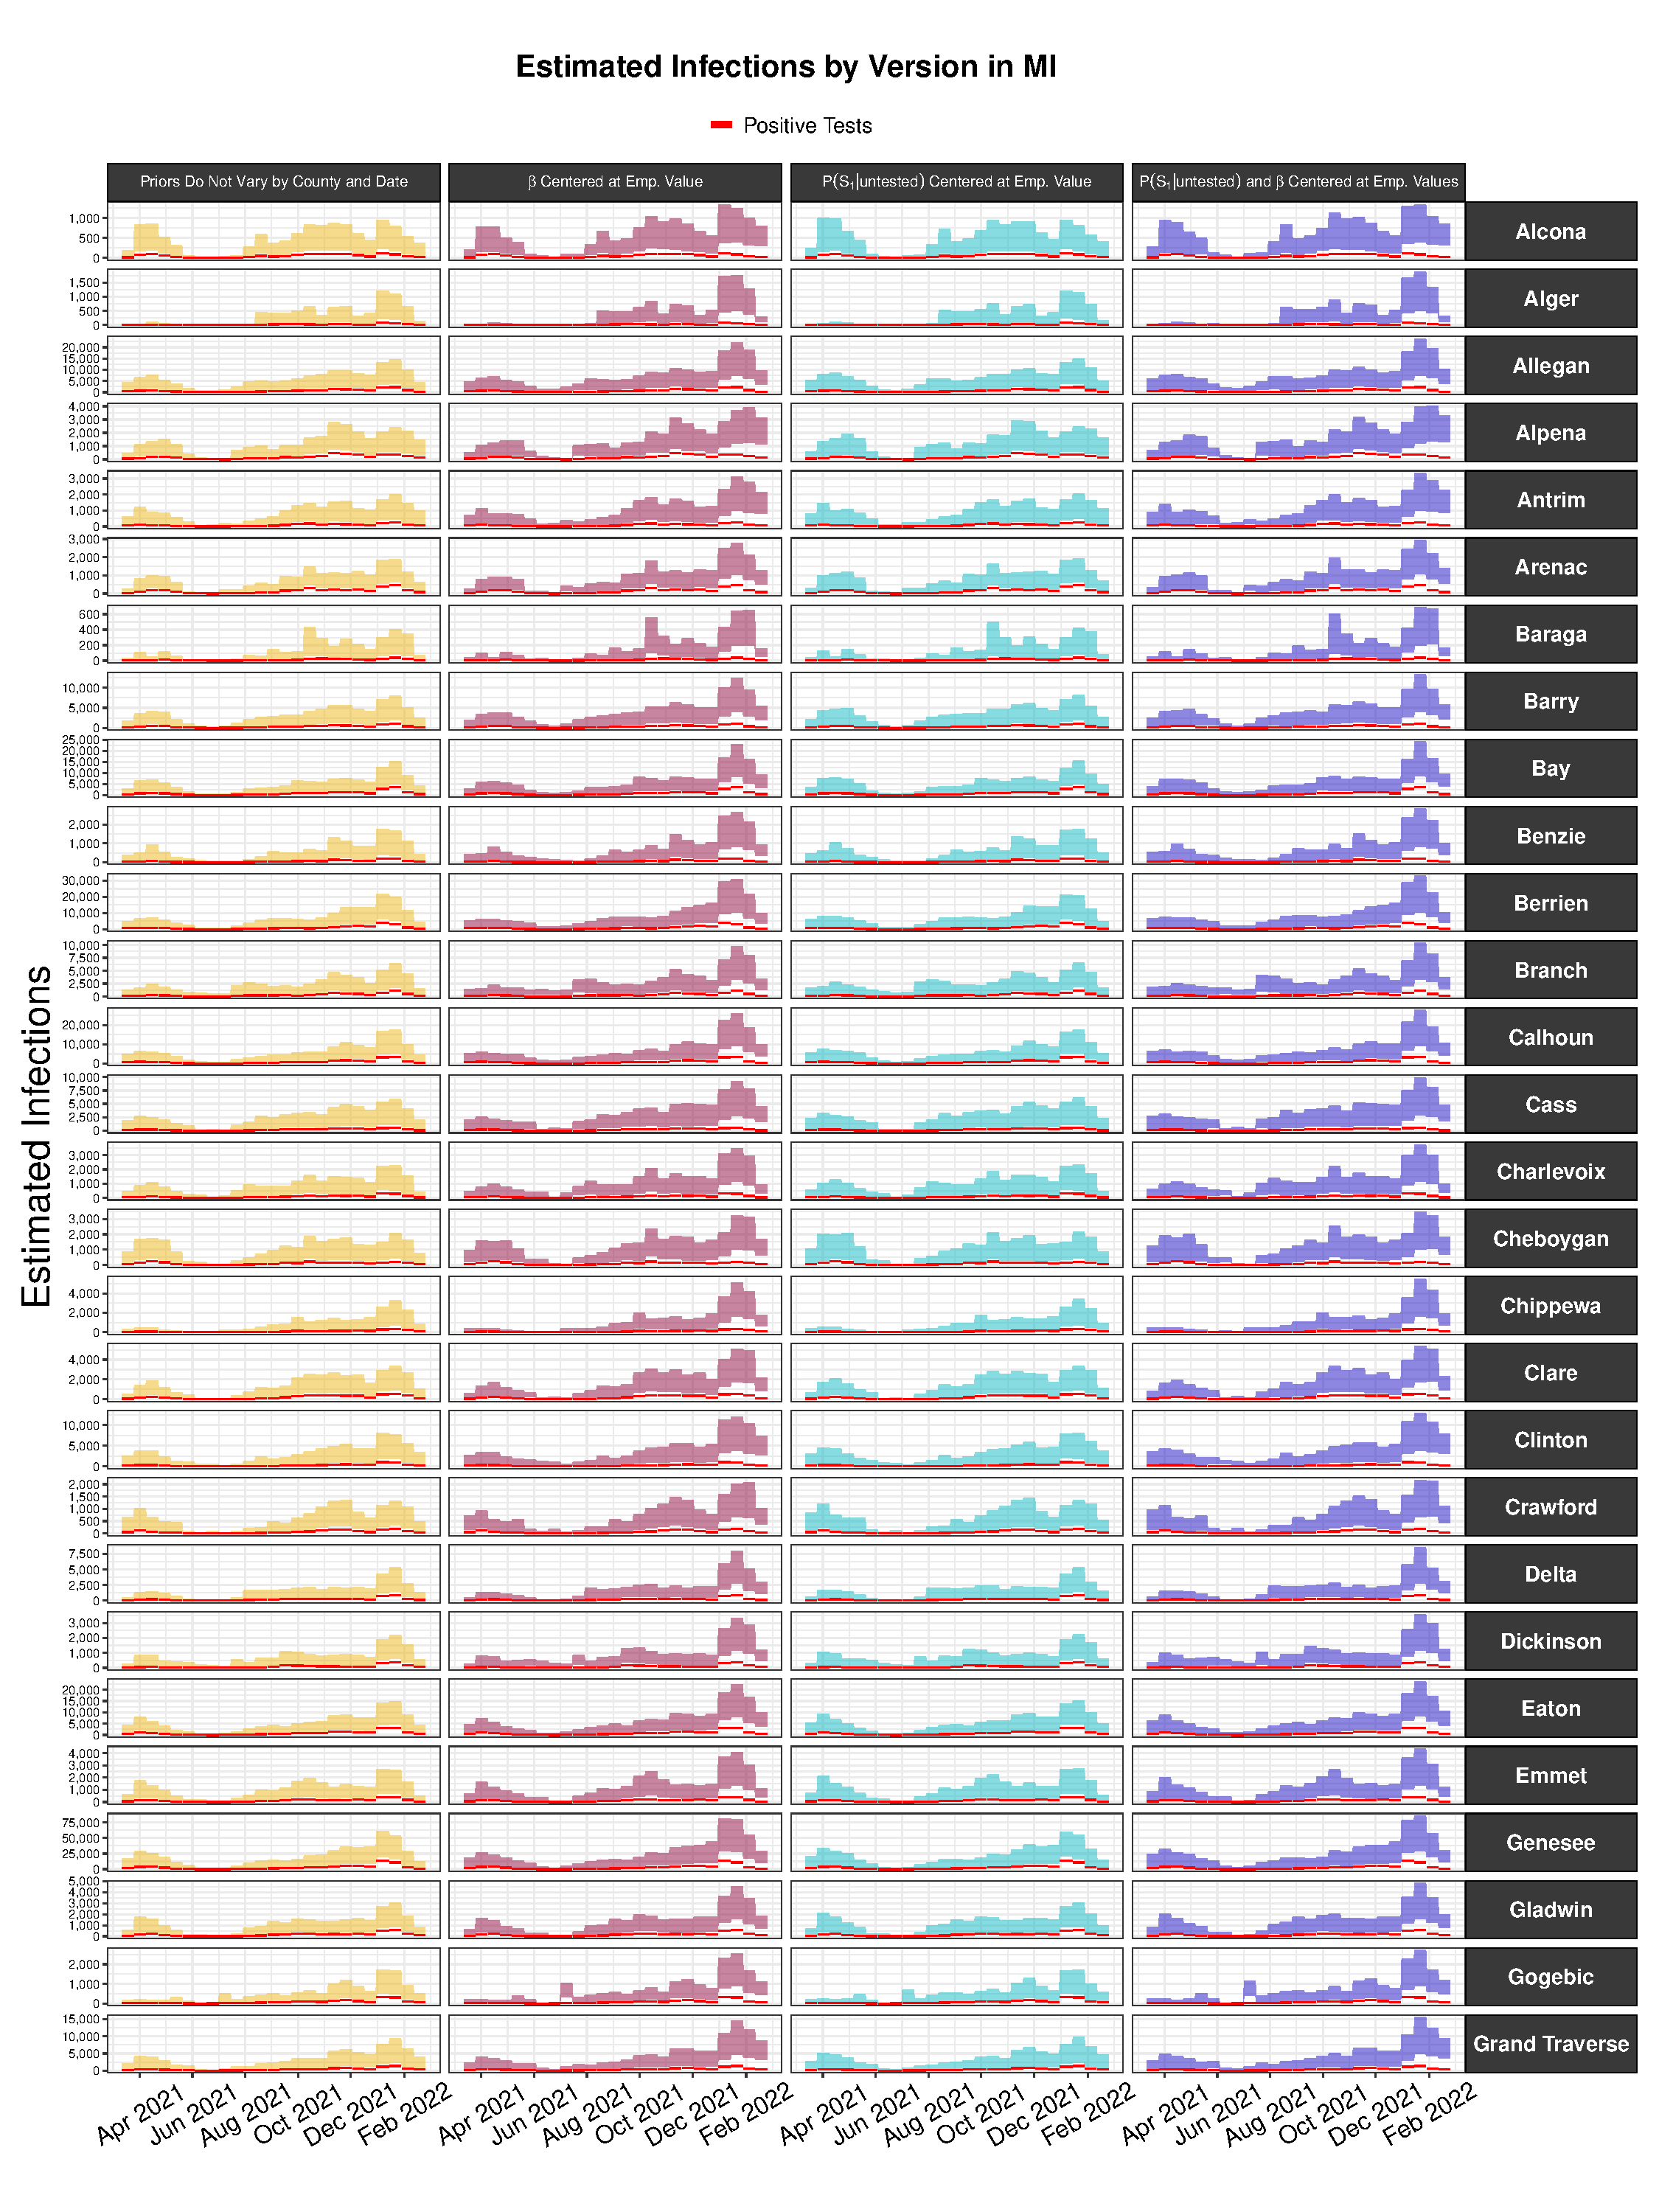
\includegraphics[width=1\linewidth]{figure/mi1_pb_compared_to_observed} \caption{\label{fig:pb_versions_mi}}\label{fig:unnamed-chunk-76-1}
\end{figure}
\begin{figure}
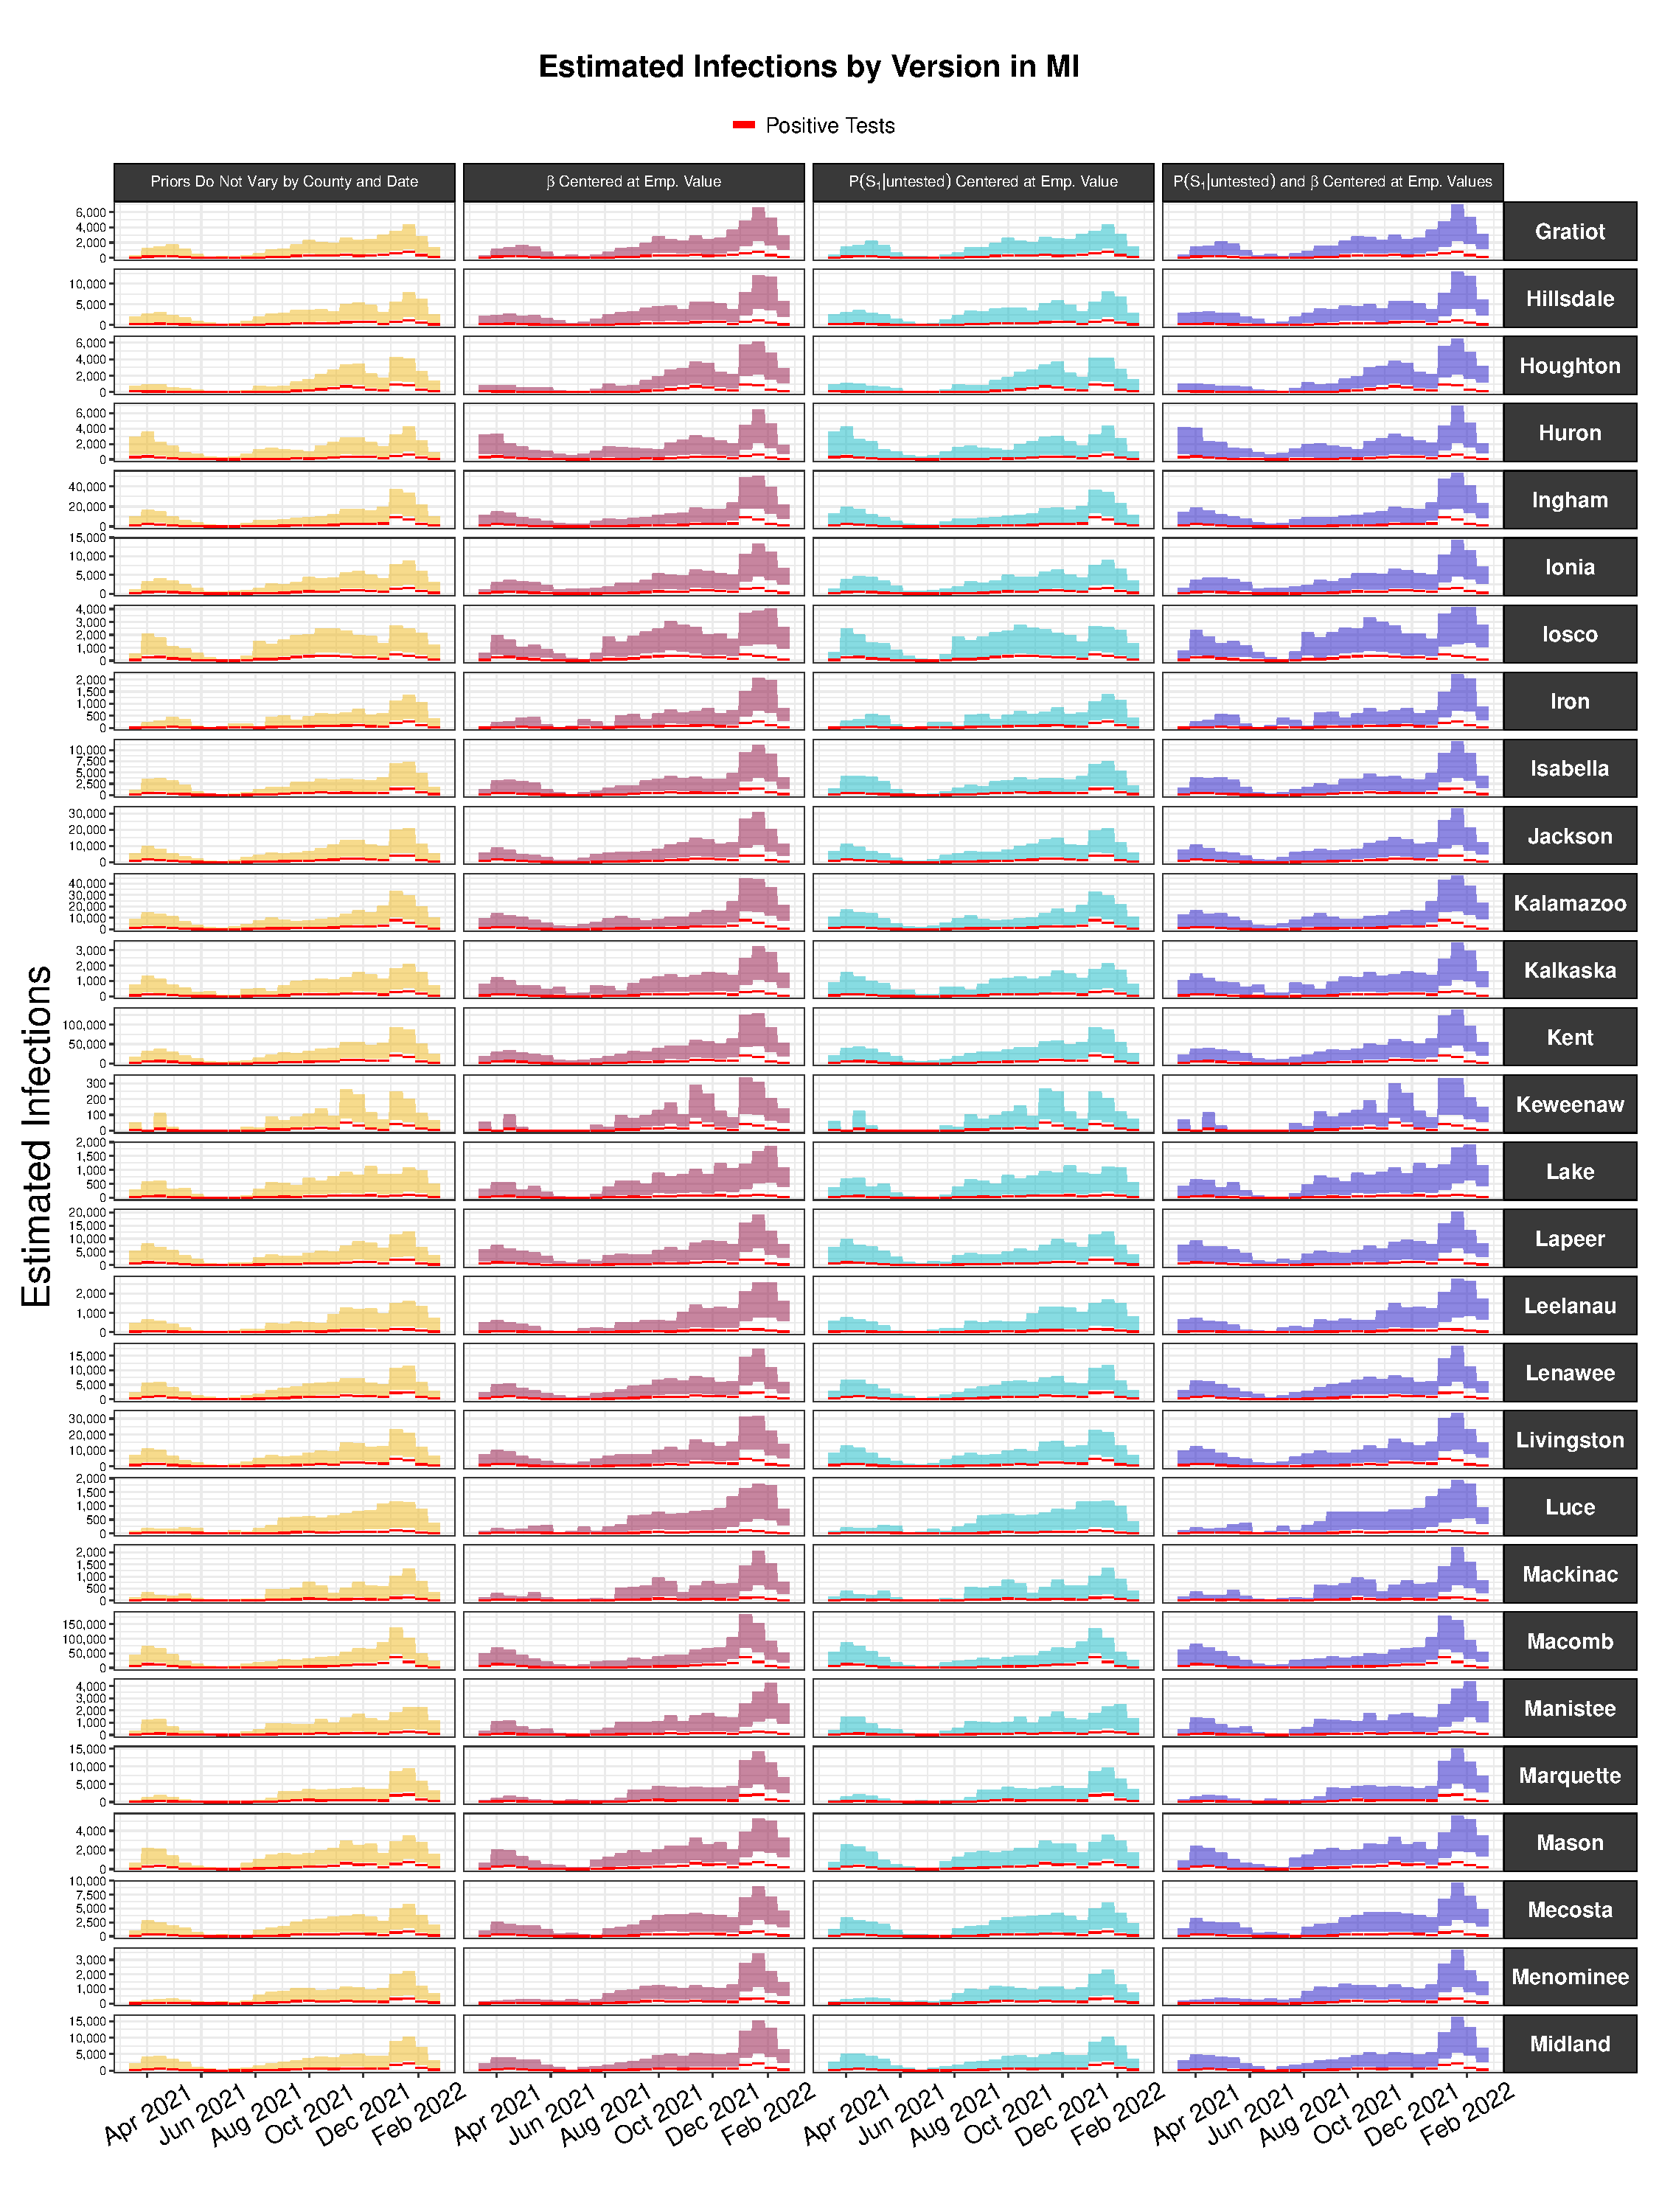
\includegraphics[width=1\linewidth]{figure/mi2_pb_compared_to_observed} \caption{\label{fig:pb_versions_mi}}\label{fig:unnamed-chunk-76-2}
\end{figure}
\begin{figure}
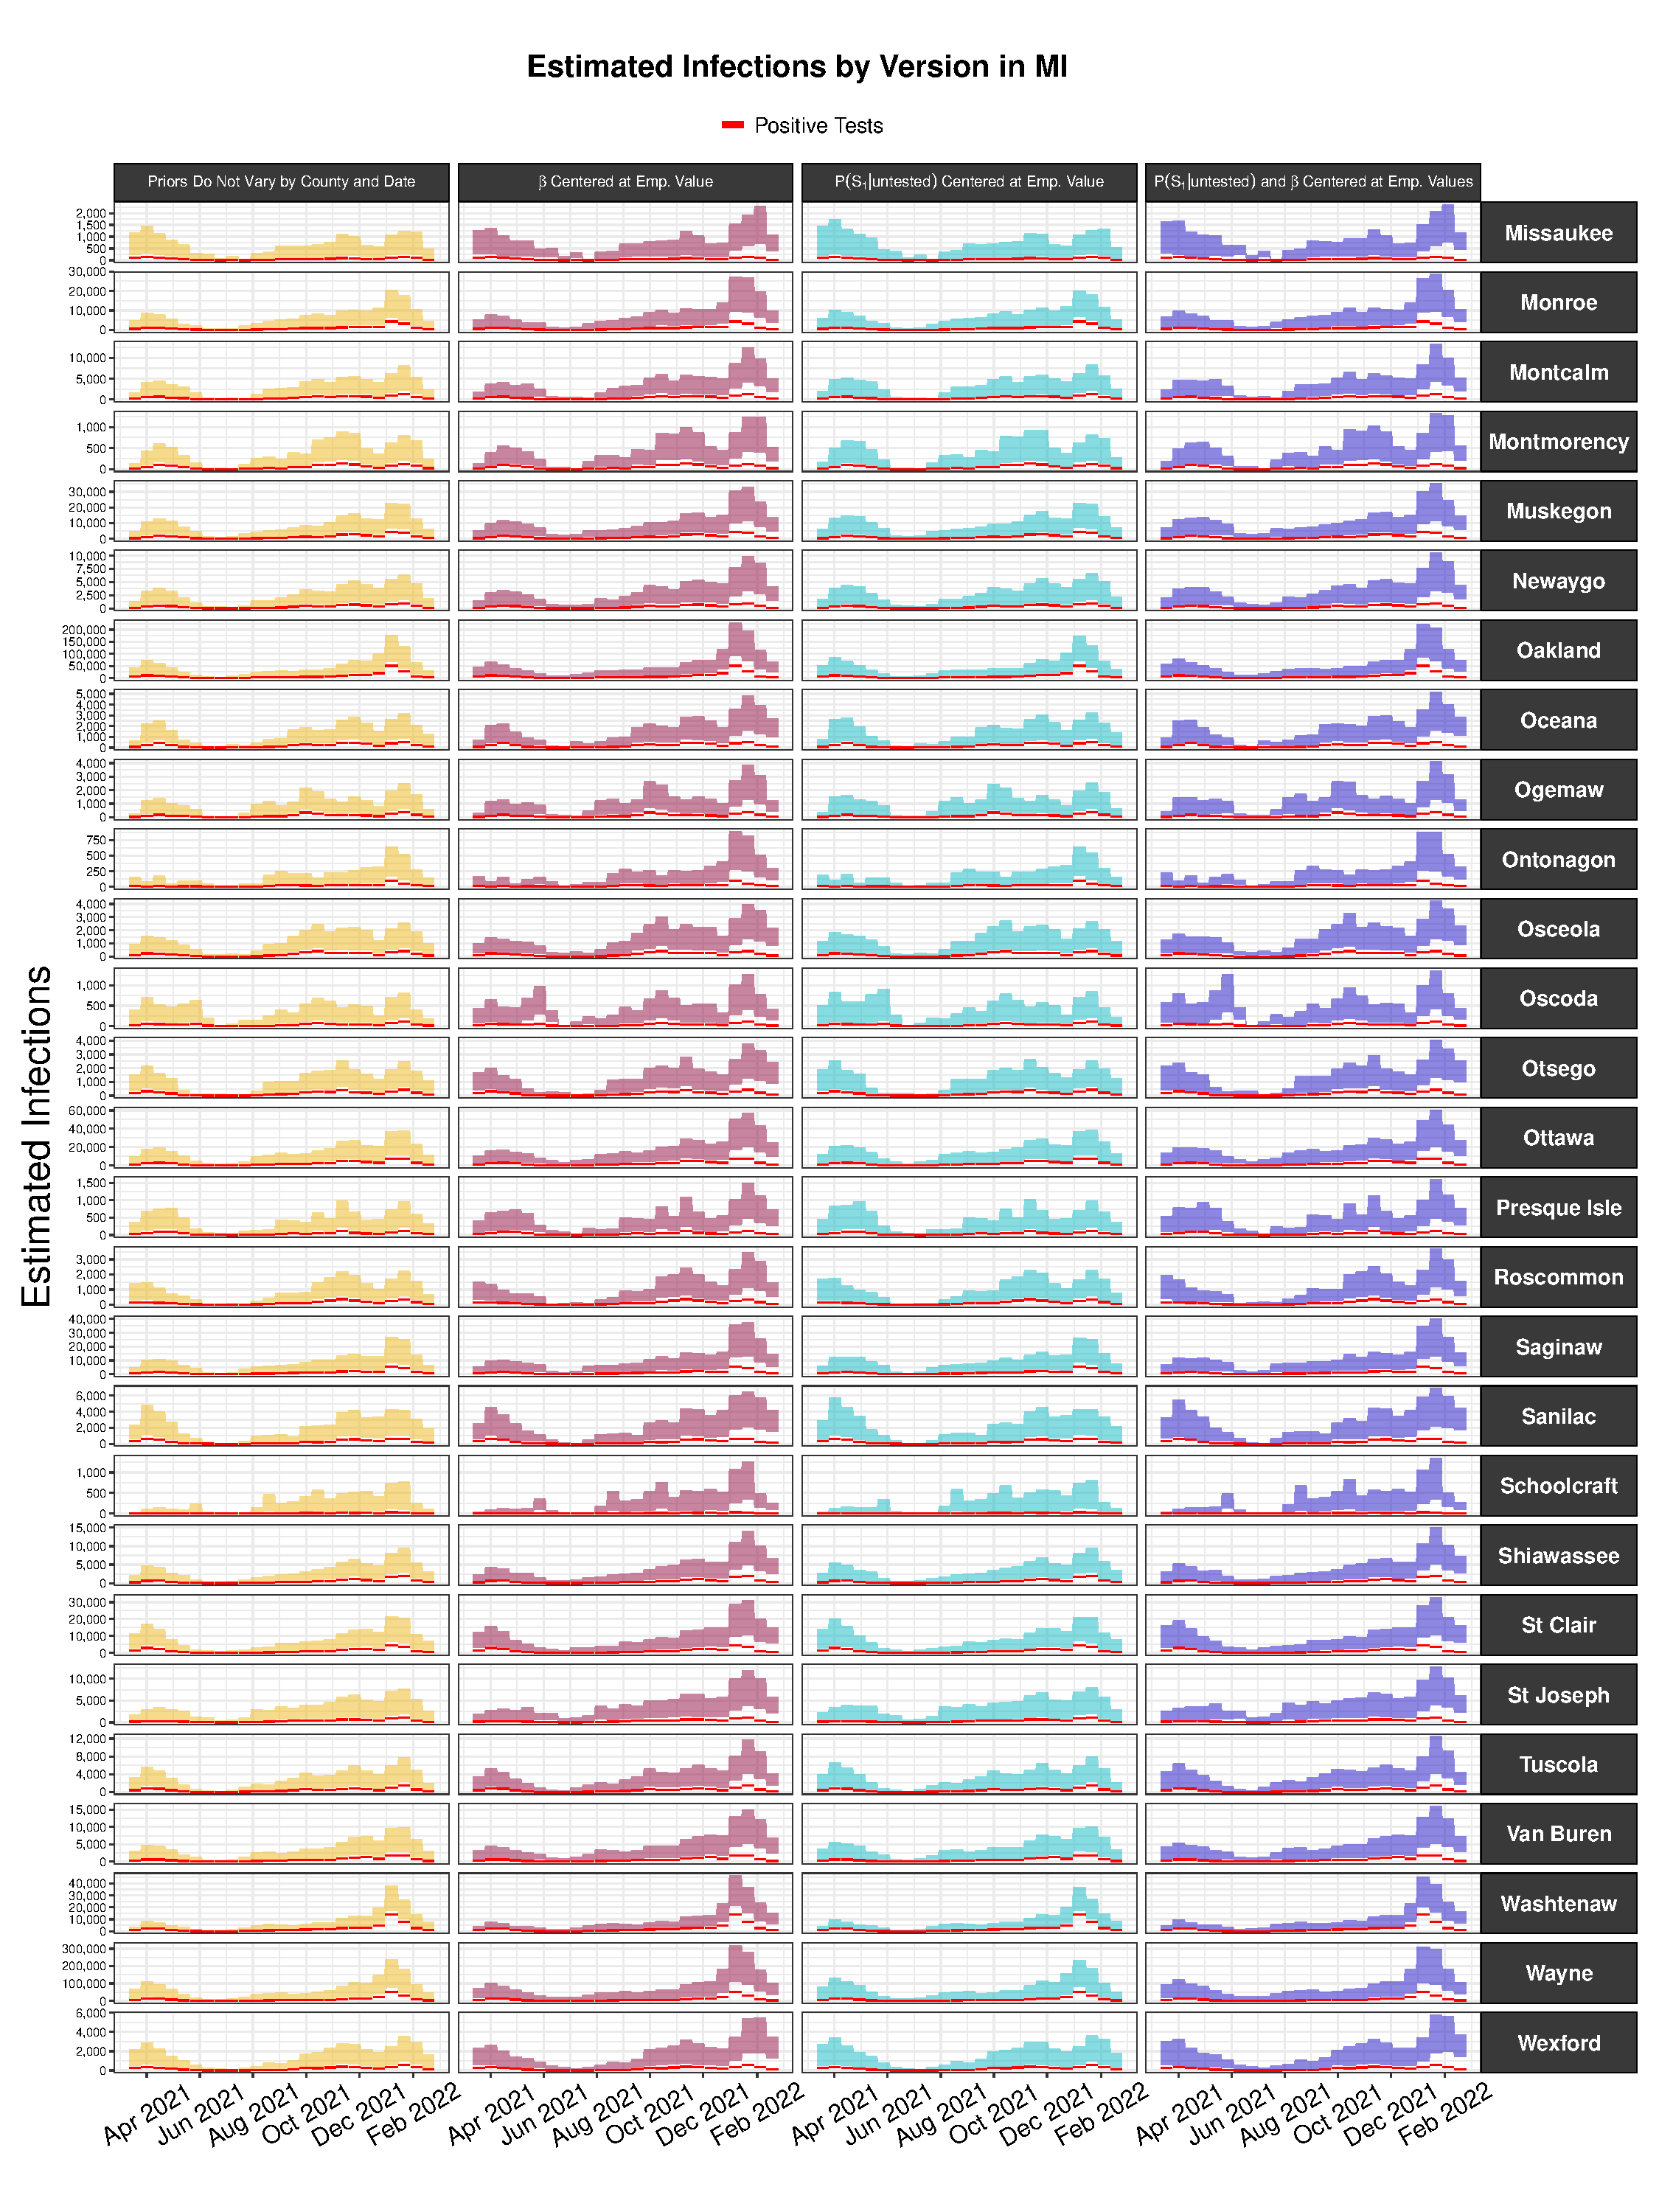
\includegraphics[width=1\linewidth]{figure/mi3_pb_compared_to_observed} \caption{\label{fig:pb_versions_mi}}\label{fig:unnamed-chunk-76-3}
\end{figure}
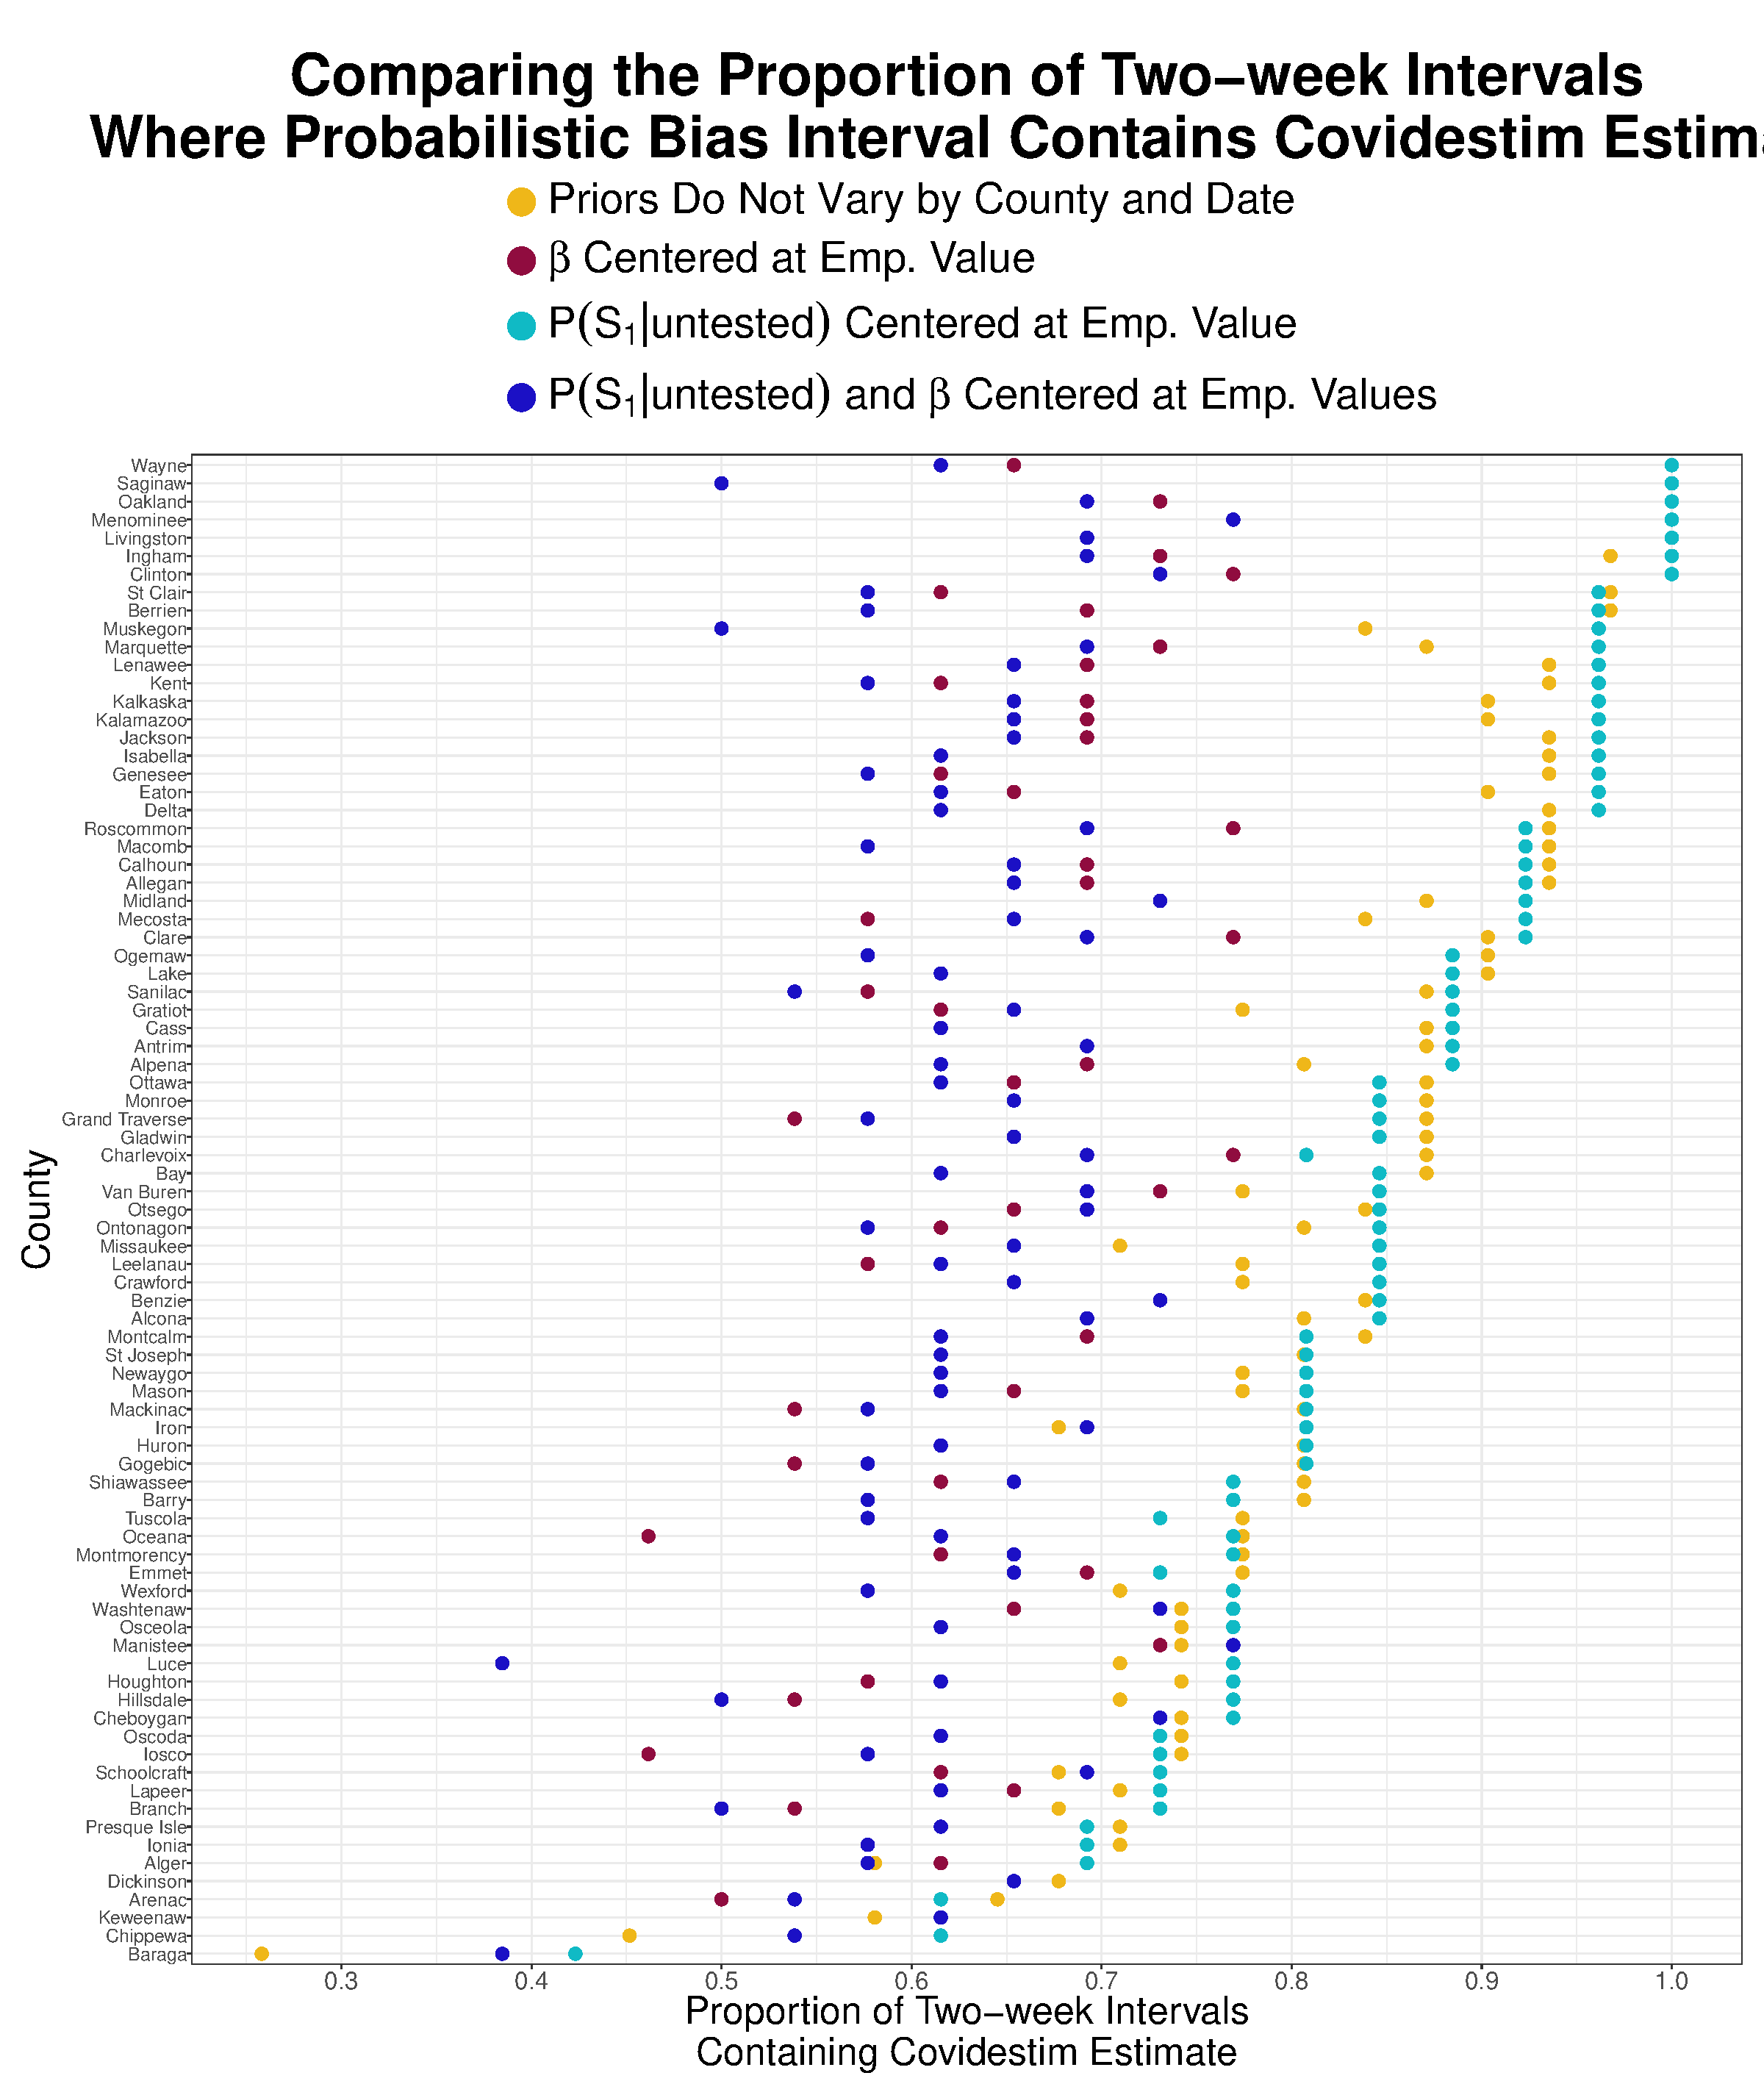
\includegraphics[width=1\linewidth]{figure/mi_pb_compared_to_covidestim_proportions}

\newpage

\hypertarget{state-level-results}{%
\section{State-level Results}\label{state-level-results}}

There is much more comprehensive testing data at the state-level than at the county level, as John Hopkins has tracked state-level testing data throughout the pandemic.
As a result, we can apply probabilistic bias analysis across the United States at the state-level.

However, since versions 2-4 of the analysis utilize empirical estimates of \(P(S_1|\text{untested})\) or \(\beta\) from the COVID-19 Trends and Impact Survey, these versions are only possible when there is sufficient data. As we see in Figure \ref{fig:statectis}, some states have very little data for the empirical estimate of beta. However in Figure \ref{fig:statectis-s-untested} we see that there is more consistent reporting of \(P(S_1|\text{untested})\).

For versions 2-4, we did not attempt the probabilistic bias analysis for states where more than 60\% of observations were missing at the daily time step. Missing values for states with sufficient data were imputed before summarizing to the biweek level using a linear weighted moving average.
\begin{figure}
\includegraphics[width=0.9\linewidth]{figure/ctis_beta_states} \caption{\label{fig:statectis}}\label{fig:unnamed-chunk-78}
\end{figure}
\begin{figure}
\includegraphics[width=0.9\linewidth]{figure/ctis_s_untested_states} \caption{\label{fig:statectis-s-untested}}\label{fig:unnamed-chunk-79}
\end{figure}
In Figures \ref{fig:state-results-1} and \ref{fig:state-results-2}, we compare the 95\% credible intervals of Covidestim summed to be on the biweek time scale to the probabilistic bias analysis intervals\footnote{As mentioned in the \protect\hyperlink{lims}{limitations} section, the two week intervals cannot be interpreted as 95\% credible intervals. However, the comparison is still useful to contextualize the results of the probabilistic bias analysis.}. We see correspondence is much higher before the Omicron wave in late 2021 through early 2022, where Covidestim estimates the cases to be much higher.
\begin{figure}
\includegraphics[width=1\linewidth]{figure/state_comp_covidestim1} \caption{\label{fig:state-results-1}}\label{fig:unnamed-chunk-80}
\end{figure}
\begin{figure}
\includegraphics[width=1\linewidth]{figure/state_comp_covidestim2} \caption{\label{fig:state-results-2}}\label{fig:unnamed-chunk-81}
\end{figure}
\hypertarget{cross-correlation-comparison}{%
\section{Cross Correlation Comparison}\label{cross-correlation-comparison}}

\hypertarget{background-1}{%
\subsection{Background}\label{background-1}}

An ongoing challenge for assessing the quality of the probabilistic bias intervals is that there is no ground truth to compare to. To broaden our comparison beyond Covidestim, we can look at wastewater data.

Wastewater data is a source of data that has been of rising interest throughout the pandemic, in part due to its cost effectiveness in assessing community-level burden, but also due to the fact it represents a much more unbiased sample than COVID-19 testing does.

That said, there are challenges in relating wastewater concentrations to the true number of infections, in part because of the same issue we face here of the lack of ground truth for the true number of infections in any location. The choice of normalization of the viral RNA concentrations of SARS-CoV-2 is important for understanding how these concentrations scale to the number of infections, since the concentration of virus (in genome copies per liter) in a sample will be influenced by various factor unrelated to the true prevalence COVID-19, such as processing differences between treatment plants or trends in water usage. One common choice is to normalize against the concentration of a virus that has a relatively stable population in wastewater, such as Pepper Mild Mottle Virus (PMMoV) (Zhan et al., 2022).

Wastewater testing has become increasingly widespread throughout the pandemic as the technology and analysis approaches have evolved, as well as the demand for a source of data on the presence of COVID-19 that is less reliant on access to tests (or symptoms strong enough to warrant a test, which differ by the variants circulating). A comprehensive source of wastewater data across the United States is provided by Biobot Analytics, which is the institution partnering with the CDC for the National Wastewater Surveillance System (NWSS) (Duvallet et al., 2022). Biobot Analytics provide wastewater concentrations aggregated at the county scale by using a weighted average of the concentrations at sampling locations within the county, weighted by the size of the corresponding sewershed populations. This data is publicly available on a public github repository.

Most notable for this work, several counties in Massachusetts have reported wastewater data for a substantial period throughout 2021 to 2022. This allows us to compare the bias-corrected estimates -- as well as the Covidestim estimates -- to the wastewater concentrations.

Wastewater concentrations are typically a leading indicator of observed cases, though there may be some variability in the lead time during different waves of the pandemic (Hopkins et al., 2023). In particular, the lead time was strongest in the earliest waves of the pandemic, and has since declined (Xiao et al., 2022). Various factors can create the changes we see in lead time over the course of the pandemic; for example, the lead time can be impacted by differences in viral shedding, diagnostic testing turnaround times, and testing capacity and behavior (Olesen, Imakaev, \& Duvallet, 2021).

Since the correlation between the time series as well as the lag at which the maximum correlation occurs are both of interest, we assessed the cross correlation between the series.

First, we define autocorrelation since the definition of cross correlation is very similar. The definition here uses the notation of Shumway \& Stoffer (2011).
\begin{tcolorbox}[title=Definition: Autocorrelation]

Denote the set of time points of a time series $T$. For any time series $(x_t)_{t\in T}$, we define the auto-correlation function (ACF)  as 

$$\rho_{XX}(\tau) = \dfrac{E[(X_{t + \tau} - \mu_{X_{t+\tau}}) (X_t - \mu_{X_t})]}{sd(X_{t+\tau}) sd(X_t)}.$$
\end{tcolorbox}
Assuming second order stationarity\footnote{Second order stationarity is also referred to as weak stationarity, and implies that the mean, variance are constant over time and the autocovariance function depends only on the difference between time points.}, we have \(\mu_{X_{t+\tau}}=\mu_{X_{t}}\)
and similarly \(\text{Var}({X_{t+\tau}})=\text{Var}({X_{t}})\), so we an simplify the expression for \(\rho_{XX} (\tau)\) to yield\\
\[\rho_{XX} (\tau)=\dfrac{E[(X_{t + \tau} - \mu_{X}) (X_t - \mu_{X})]}{Var(X)}.\]

The auto-correlation function \(\rho_{XX}(\tau)\) measures the linear dependence between \(X_{1+\tau}, \dots X_n\) and \(X_1, \dots, X_{n-\tau}\), that is, the difference between the original time series and the time series shifted forward by \(\tau\) time units.

We can extend this definition to quantify the linear relationship between distinct lagged time series \(X_1, X_2, \dots, X_t\) and \(Y_1, Y_2, \dots, Y_t\) by defining the cross correlation function. The function is only defined on two time series that are over the same time interval and sampled at the same frequency.
\begin{tcolorbox}[title=Definition: Cross-Correlation]

We compute the cross-correlation function (CCF) as

$$\rho_{XY}(s,t) = \dfrac{E[(X_s - \mu_{X_s})(Y_t-\mu_{Y_t})]}{\sqrt{\text{Var}(X_s) \text{Var}(Y_t)}}.$$
Again assuming the series satisfy second-order stationarity, we have

$$\rho_{XY}(s,t) = \dfrac{E[(X_s - \mu_{X})(Y_t-\mu_{Y})]}{\sqrt{\text{Var}(X) \text{Var}(Y)}}.$$

\end{tcolorbox}
The implementation of the cross correlation in base R (\texttt{stats::ccf}) assumes second order stationarity (Venables \& Ripley, 2002).

Looking at cross correlation can be useful in the sense that we can both consider the strength of correlation and the lag at which the correlation is maximized. Before presenting the cross correlation results of the county level time series, we can consider a more concrete example, where the lag is known.

In Figure \ref{fig:compdiff}, we consider simulated data where \((Z_t)\) is \((Y_t)\) lagged by 3 time units with noise added. We can see that \(Z_t\) and \(Y_t\) are not second-order stationary since the mean clearly is not constant over time. However, to stabilize the mean, we can apply first order differencing, where we take the differences between consecutive observations.
\begin{figure}
\includegraphics[width=1\linewidth]{thesis_files/figure-latex/unnamed-chunk-82-1} \caption{\label{fig:compdiff}}\label{fig:unnamed-chunk-82}
\end{figure}
We can see the effect of applying differencing to the time series when we compute the cross correlations of \((Z_t)\) and \((Y_t)\), as shown in Figure \ref{fig:corzy}. The true lag of \(-3\) time units was recovered when considering the differenced time series, but not when we considered the original time series. In what follows, because the time series we are considering are not stationary, we consider the cross correlation between the differenced time series.
\vspace{5 cm}
\begin{figure}
\includegraphics[width=0.45\linewidth]{thesis_files/figure-latex/unnamed-chunk-83-1} \includegraphics[width=0.45\linewidth]{thesis_files/figure-latex/unnamed-chunk-83-2} \caption{\label{fig:corzy}}\label{fig:unnamed-chunk-83}
\end{figure}
\hypertarget{cross-correlation-results-comparing-bias-corrected-counts-covidestim-estimates-and-wastewater-concentrations}{%
\subsection{Cross Correlation Results Comparing Bias Corrected Counts, Covidestim Estimates, and Wastewater Concentrations}\label{cross-correlation-results-comparing-bias-corrected-counts-covidestim-estimates-and-wastewater-concentrations}}

Because wastewater data is reported at the weekly time scale while the bias corrected estimates are at the 2-week time scale, we take a mean of the effective concentration for each 2 week interval, such that the time series are sampled at the same frequency.\footnote{We cannot interpret the cross correlation if the time steps are different.}

Since the effective concentration of SARS-CoV-2 in wastewater samples reported by Biobot is in genome copies per liter and is not directly comparable to estimates of infections, we place the wastewater concentration on a separate scale.

Looking at the counties in Figure \ref{fig:wastewater_ma_by_county}, we see that, with the exception of Barnstable, MA, the wastewater trends are highly similar to trends captured by the bias corrected infection counts. We also see that the trends are similar both with regard to shape but also with regard to time, with little visible lag between the series. This is expected because although wastewater cases do in general lead cases, lead times generally are not on the order of 2 weeks. This means that since we are summarizing to 2-week intervals we would expect the lag to be very small, if present at all.
\begin{figure}
\includegraphics[width=1\linewidth]{figure/wastewater_ma_by_county} \caption{\label{fig:wastewater_ma_by_county}}\label{fig:unnamed-chunk-84}
\end{figure}
\hypertarget{comparison-between-implementations-of-probabilistic-bias-analysis}{%
\subsubsection{Comparison Between Implementations of Probabilistic Bias Analysis}\label{comparison-between-implementations-of-probabilistic-bias-analysis}}

In Figure \ref{fig:correlation_observed_pb}, we see that, in general, infections were highly correlated with the wastewater effective concentrations, which was true across all implementations of probabilistic bias analysis. In most cases, the implementation where priors did not vary by state or date were the most highly correlated with the wastewater concentrations. Exceptions to this were Barnstable County (25001), where the implementation with the prior for \(\beta\) centered at the empirical value was the most highly correlated, and Worcester County (25027), where the implementation with the prior for \(P(S_1|\text{untested})\) centered at empirical value was the most highly correlated. In all counties except for Barnstable, the lag at which the maximum correlation was obtained was 0 units, while for Barnstable it was -1, indicating that wastewater concentrations led infections by one two-week interval.

Given the small size of Barnstable relative to other counties and high variability in its early estimates in 2021 (as seen in Figure \ref{fig:wastewater_ma_by_county}), it is possible that there were still aspects of the SARS-CoV-2 detection process that took time to refine. Another possibility is that the way Biobot aggregated wastewater concentrations by county failed to capture the infection dynamics in this county, since wastewater catchments are not contained within county lines. This is a central challenge in relating cases to wastewater concentrations, since these values are recorded for distinct geographic units.

Comparing the maximum correlations obtained the observed cases, only in Hampshire County were the observed cases more correlated with the wastewater concentrations than all implementations of probabilistic bias analysis. We also see again that in most cases the maximum correlation is obtained at zero lag in observed cases; however, for Barnstable, the correlation is highest when wastewater concentrations lead infections by two biweeks, and for Hampshire the correlation is highest when wastewater concentrations lead infections by 1 biweek.
\begin{figure}
\includegraphics[width=1\linewidth]{figure/correlation_observed_pb} \caption{\label{fig:correlation_observed_pb}}\label{fig:unnamed-chunk-85}
\end{figure}
\hypertarget{comparison-between-covidestim-observed-cases-and-bias-corrected-counts}{%
\subsubsection{Comparison Between Covidestim, Observed Cases, and Bias Corrected Counts}\label{comparison-between-covidestim-observed-cases-and-bias-corrected-counts}}

In Figure \ref{fig:correlation_observed_pb_covidestim}, we also compare the Covidestim estimates to the wastewater concentrations. In general, both Covidestim and bias-corrected counts are more correlated with wastewater concentrations than observed infections. Of note, Nantucket County (25019) is not included here because Covidestim does not report estimates are not reported for Nantucket.\footnote{In reporting of COVID-19 data, Nantucket values are grouped with Dukes County, which is likely why Covidestim does not try to estimate the grouped counts.}
\begin{figure}
\includegraphics[width=1\linewidth]{figure/correlation_observed_pb_covidestim} \caption{\label{fig:correlation_observed_pb_covidestim}}\label{fig:unnamed-chunk-86}
\end{figure}
\hypertarget{takeaways}{%
\subsubsection{Takeaways}\label{takeaways}}

The aim of the cross correlation analysis was to add another source of comparison for the county-level counts from an entirely different source of data -- in particular, a source of data that is less impacted by access to testing or test behavior. We see that in most counties considered here, there is high agreement between the time series. An avenue for future exploration would be to consider this analysis among a broader set of counties to see which time series tends to be most highly correlated with wastewater concentrations, a question that we cannot confidently address here when looking only at counties in Massachusetts.

\hypertarget{conclusion}{%
\chapter{Conclusion}\label{conclusion}}

The aim of this work is to consider possible scenarios for the extent of unobserved infections over an extended time during the COVID-19 pandemic, and to explore how we can present the uncertainty in the number of incident infections. Throughout the pandemic we often see line charts of observed cases or the test positivity rate. Advice has changed as has testing behavior, with warnings to not consider case counts in isolation, but rather to also look at trends in the test positivity rate (among other indicators). However, presentation of infections as intervals, their widths defined as a direct consequence of assumptions we make about the bias parameters, reflects genuine uncertainty about the number of true infections that may exist in a given area over time.
Various models exist to try to get at this quantity of the number of true infections, incorporating a range of sources of data, including COVID-19 deaths, hospitalizations, seroprevalence data, and viral concentrations in wastewater, as well as estimates such as the infection fatality ratio.
The strength of applying probabilistic bias analysis to consider possible values of true COVID-19 infections lays in its relative simplicity and transparency of assumptions, in addition to the ease of exploration of possible testing scenarios of the extent to which infections are going undetected. Although there is no ground truth to rigorously assess the accuracy of an estimate of the true number of COVID-19 infections, comparing approaches and understanding where and when they are non concordant provides useful insight into quantifying the range of true infections.

\appendix

\hypertarget{appendix}{%
\chapter{Appendix}\label{appendix}}

\hypertarget{smoothing-span}{%
\section{Smoothing Span}\label{smoothing-span}}

\hypertarget{changing-span-for-loess-smoothing-of-beta}{%
\subsection{\texorpdfstring{Changing SPAN for LOESS Smoothing of \(\beta\)}{Changing SPAN for LOESS Smoothing of \textbackslash beta}}\label{changing-span-for-loess-smoothing-of-beta}}

\hypertarget{changing-mean-and-variance-for-prior-distribution-specifications}{%
\section{Changing Mean and Variance for Prior Distribution Specifications}\label{changing-mean-and-variance-for-prior-distribution-specifications}}

\hypertarget{relationship-between-xy_alpha-and-x_alpha-y_alpha-for-dependent-variables-xy}{%
\section{\texorpdfstring{Relationship Between \((X+Y)_\alpha\) and \(X_{\alpha}\) +\(Y_{\alpha}\) for Dependent Variables \(X,Y\)}{Relationship Between (X+Y)\_\textbackslash alpha and X\_\{\textbackslash alpha\} +Y\_\{\textbackslash alpha\} for Dependent Variables X,Y}}\label{relationship-between-xy_alpha-and-x_alpha-y_alpha-for-dependent-variables-xy}}

\hypertarget{simulation-bivariate-normal}{%
\subsection{Simulation: Bivariate Normal}\label{simulation-bivariate-normal}}

We can see this in a concrete example. Let \((X,Y)\) be bivariate normal with \(\boldsymbol \mu = \begin{pmatrix} 0\\0\end{pmatrix}\) and correlation matrix \(\boldsymbol \Sigma = \begin{pmatrix} 1 & \rho \\ \rho & 1 \end{pmatrix}\), and hence where \(X, Y\) are marginally standard normal random variables.

We let the subscript \(\alpha\) denote the \(\alpha^{th}\) and the subscript \(1-\alpha\) denote the \((1-\alpha)^{th}\) quantile of the distribution.

In Figure \ref{fig:simmvn}, in each panel, we increase the correlation \(\rho\) between \(X\) and \(Y\) by 0.25 units and plot the sum \(X +Y\) against \(X\). The vertical lines represent quantiles \(X_{0.025}\) and \(X_{0.975}\), and the horizontal lines represent the quantiles \((X+Y)_{0.025}\) and \((X+Y)_{0.975}\).

We see in Figure \ref{fig:simmvn} that when we increase the correlation between \(X\) and \(Y\), the width of the interval \(\Big((X+Y)_\alpha, (X+Y)_{1-\alpha}\Big)\) increases.
\begin{figure}

{\centering \includegraphics[width=0.96\linewidth]{thesis_files/figure-latex/unnamed-chunk-88-1} \includegraphics[width=0.96\linewidth]{thesis_files/figure-latex/unnamed-chunk-88-2} \includegraphics[width=0.96\linewidth]{thesis_files/figure-latex/unnamed-chunk-88-3} \includegraphics[width=0.96\linewidth]{thesis_files/figure-latex/unnamed-chunk-88-4} \includegraphics[width=0.96\linewidth]{thesis_files/figure-latex/unnamed-chunk-88-5} 

}

\caption{\label{fig:simmvn}}\label{fig:unnamed-chunk-88}
\end{figure}
In Figure \ref{fig:comp-intervals}, we compare the intervals defined by taking the quantiles of the sum, \(\Big((X+Y)_\alpha, (X+Y)_{1-\alpha}\Big)\), to the intervals taken by summing the quantiles individually, \(\Big(X_\alpha +Y_\alpha, \; X_{1-\alpha} +Y_{1-\alpha}\Big)\). We notice that, as we saw in Figure \ref{fig:simmvn}, increasing the correlation increases the width of the interval \(\Big((X+Y)_\alpha, (X+Y)_{1-\alpha}\Big)\), while the interval \(\Big(X_\alpha +Y_\alpha, \; X_{1-\alpha} +Y_{1-\alpha}\Big)\) is constant since changing the correlation does not change the marginal quantiles \(X_\alpha, X_{1-\alpha}\).,
\begin{figure}

{\centering \includegraphics[width=1\linewidth]{thesis_files/figure-latex/unnamed-chunk-89-1} 

}

\caption{\label{fig:comp-intervals}}\label{fig:unnamed-chunk-89}
\end{figure}
As we see in Figure \ref{fig:comp-intervals}, the intervals are identical when \(X,Y\) are perfectly correlated. This result is not dependent on the choice of distribution, as we can show by considering CDFs and quantile functions of a general distribution.
\begin{tcolorbox}[title = Quantiles of the Sum of Perfectly Correlated Random Variables]
When two random variables $X$ and $Y$ are perfectly correlated,
$$X_\alpha + Y_\alpha = (X+Y)_\alpha.$$
\end{tcolorbox}
When \(X\) and \(Y\) are perfectly correlated, \(Y\) must be a linear combination of \(X\), so we can write \(X+Y= X+bX=(1+b)X\).

Then, let the \(\alpha^{th}\) quantile of \((1+b)X\) be \(x_\alpha\). By definition of the quantile function, we have

\[F^{-1}_{(1+b) X } (\alpha) = x_\alpha \implies P((1+b) X \leq x_\alpha) = \alpha.\]
Since \((1+b)\) is just a constant, we can divide to yield

\[P\Big( X \leq x_\alpha/(1+b) \Big) = \alpha.\]
To optain hte quantile for \(bX\), we can multiply each side by \(b\) to yield
\[P\Big( bX \leq bx_\alpha/(1+b) \Big) = \alpha.\]
Putting these results together, we have
\begin{align*}
F^{-1}_{bX} (\alpha) + F^{-1}_{X} (\alpha) = \frac{bx_\alpha } { 1+b} + \frac{x_\alpha}{1+b}
&= x_\alpha 
&= F^{-1}_{(1+b)X}(\alpha) \end{align*}

\hypertarget{conservativeintervals}{%
\subsection{Derivation of the Distribution of X+Y for Bivariate Normal}\label{conservativeintervals}}

We can see why we observe this relationship between intervals based on the the sum of the \(\alpha^{th}\) quantiles of the individual distributions, \(X_\alpha + Y_\alpha\), and the intervals based on the \(\alpha^{th}\) quantile of the distribution of \(X+Y\) by considering the definition of the quantile function of the normal distribution.

Defining \(Z=g(X,Y) = X+Y\), we can obtain the density function by a change of variables. Notice if \(g(X,Y) = X+Y\), \(g^{-1}(X,Z) = Z-X\), so we have
\begin{align*} f_{X,Z}(x,z) &= f_{X,Y}(x,g^{-1}(x,z)) \left|\frac{\partial g^{-1}(x,z)}{\partial z}\right| \\
f_{X,Z}(x,z) &= f_{X,Y}(x,z-x) \left|\frac{\partial (x-z)}{\partial z}\right|\\
f_{X,Z}(x,z) &= f_{X,Y}(x,z-x) \left|1\right|\\
f_{X,Z}(x,z) &= f_{X,Y}(x,z-x) \\
\end{align*}
Then, we can marginalize out \(X\) to get the PDF of \(f_Z\) by taking

\[f_Z(z) = \int_{\infty}^\infty f(x,z-x) \; dx.\]

Since \((X,Y)\) is bivariate normal with correlation \(\rho\), the PDF is given by

\[f(x,y) = \dfrac{exp\left[\dfrac{-1}{2(1-\rho^2)} \left( \dfrac{(x-\bar x)^2}{\sigma_x^2}+\dfrac{(y-\bar y)^2}{\sigma_x^2} - \dfrac{2 \rho (x-\bar x)(y-\bar y)}{\sigma_x\sigma_y} \right)\right]}{2\pi \sigma_x \sigma_y \sqrt{1- \rho^2}}\]

Integrating with respect to \(x\)\footnote{This integration is extremely long and technical, so we do not include it here.}, we have

\[f_Z(z)  = \int_{-\infty}^\infty \dfrac{\exp\left[\dfrac{-1}{2(1-\rho^2)} \left( \dfrac{(x-\bar x)^2}{\sigma_x^2}+\dfrac{(y-\bar y)^2}{\sigma_x^2} - \dfrac{2 \rho (x-\bar x)(z-x-\bar y)}{\sigma_x\sigma_y} \right)\right]}{2\pi \sigma_x \sigma_y \sqrt{1- \rho^2}} dx \]
\[=\dfrac{\exp\left[-\dfrac{(z-(\bar x + \bar y ))^2}{2(\sigma^2_x+\sigma^2_y + 2\rho \sigma_x \sigma_y)}\right]}{\sqrt{2\pi(\sigma_x^2 + \sigma_y^2 + 2\rho \sigma_x \sigma_y)}}.\]
It follows that \(Z\) is a normal random variable with mean \(\bar x + \bar y\) and standard deviation \(\sqrt{\sigma_x^2 +\sigma_y^2 + 2 \rho \sigma_x \sigma_y }\).

In Figure \ref{fig:ex-sim-normal}, we plot the density estimate of the distribution of \(X+Y\) for \((X,Y) \sim MVN\left( \begin{pmatrix} 0\\0 \end{pmatrix}, \begin{pmatrix} 1 & 0.2 \\0.2 & 1 \end{pmatrix}\right)\) and plot the density of the random variable \(X+Y = Z \sim N\left(\bar x + \bar y,\sqrt{\sigma_x^2 +\sigma_y^2 + 2 \rho \sigma_x \sigma_y }\right)\) and see they are in close alignment, as expected.
\begin{figure}

{\centering \includegraphics[width=1\linewidth]{thesis_files/figure-latex/unnamed-chunk-92-1} 

}

\caption{\label{fig:ex-sim-normal} The theoretical density of $N\left(\bar x + \bar y,\sqrt{\sigma_x^2 +\sigma_y^2 + 2 \rho \sigma_x \sigma_y }\right)$ is plotted in red over the kernel density estimate of the observed distribution of $X+Y$.}\label{fig:unnamed-chunk-92}
\end{figure}
Since we now know \(Z \sim N\left(\bar x + \bar y,\sqrt{\sigma_x^2 +\sigma_y^2 + 2 \rho \sigma_x \sigma_y }\right)\), we can consider the quantile function of the normal distribution, which is defined as

\[F_Z^{-1}(\alpha)=\mu +\sigma_Z \; \text{erf}^{-1}(2\alpha - 1).\]
and since \(\sigma_Z=\sqrt{\sigma_x^2 +\sigma_y^2 + 2 \rho \sigma_x \sigma_y }\) we have
\[F_Z^{-1}(\alpha)=\mu + \left(\sqrt{\sigma_x^2 +\sigma_y^2 + 2 \rho \sigma_x \sigma_y } \right) \; \text{erf}^{-1}(2\alpha - 1).\]
Now, we note the inverse error function \(\text{erf}^{-1}\) is increasing (Figure \ref{fig:erf}).

This means if \(\alpha > 0.5\), \(F_Z^{-1}\) is increasing with increasing values of \(\rho\), and if \(\alpha < 0.5\), \(F_Z^{-1}\) is decreasing with increasing values of \(\rho\).

This means that if we have a pair of correlated random variables \((X_1,Y_1)\) and \((X_2,Y_2)\) and \(\rho_{X_1,Y_1} > \rho_{X_2,Y_2}\) and consider \(\alpha < 0.5\),

\[(X_1+Y_1)_\alpha <(X_2+Y_2)_\alpha\]

and

\[(X_1+Y_1)_{1-\alpha} > (X_2+Y_2)_{1-\alpha}.\]
This is exactly what we observed in Figure \ref{fig:comp-intervals}.
\begin{figure}

{\centering \includegraphics[width=1\linewidth]{thesis_files/figure-latex/unnamed-chunk-93-1} 

}

\caption{\label{fig:erf}}\label{fig:unnamed-chunk-93}
\end{figure}
\backmatter

\hypertarget{references}{%
\chapter*{References}\label{references}}
\addcontentsline{toc}{chapter}{References}

\markboth{References}{References}

\noindent

\setlength{\parindent}{-0.20in}
\setlength{\leftskip}{0.20in}
\setlength{\parskip}{8pt}

\hypertarget{refs}{}
\begin{CSLReferences}{1}{0}
\leavevmode\vadjust pre{\hypertarget{ref-aurelienpelissier2022}{}}%
Aurelien Pelissier. (2022, February 4). Density {Estimation} for {Bounded Variables}. Retrieved March 19, 2023, from \url{https://medium.com/mlearning-ai/density-estimation-for-bounded-variables-7d68f633e772}

\leavevmode\vadjust pre{\hypertarget{ref-blitzsteinIntroductionProbability2019}{}}%
Blitzstein, J. K., \& Hwang, J. (2019). \emph{Introduction to probability} (Second edition). {Boca Raton}: {CRC Press}.

\leavevmode\vadjust pre{\hypertarget{ref-californiadepartmentofpublichealth2021}{}}%
California Department of Public Health. (2021, June 15). Blueprint for a {Safer Economy}. Retrieved December 16, 2022, from \url{https://www.cdph.ca.gov/Programs/CID/DCDC/Pages/COVID-19/COVID19CountyMonitoringOverview.aspx}

\leavevmode\vadjust pre{\hypertarget{ref-carvalho2023}{}}%
Carvalho, L. M., Villela, D. A. M., Coelho, F. C., \& Bastos, L. S. (2023). Bayesian {Inference} for the {Weights} in {Logarithmic Pooling}. \emph{Bayesian Analysis}, \emph{18}(1). http://doi.org/\href{https://doi.org/10.1214/22-BA1311}{10.1214/22-BA1311}

\leavevmode\vadjust pre{\hypertarget{ref-cdc2020}{}}%
CDC. (2020, February 11). Cases, data, and surveillance to track and analyze {COVID-19}. Retrieved April 12, 2023, from \url{https://www.cdc.gov/coronavirus/2019-ncov/covid-data/serology-surveillance/index.html}

\leavevmode\vadjust pre{\hypertarget{ref-chambers1997}{}}%
Chambers, J. M. (Ed.). (1997). \emph{Statistical models in {S}} (Reprint). {London}: {Chapman \& Hall}.

\leavevmode\vadjust pre{\hypertarget{ref-chandler2021}{}}%
Chandler, C. M., Bourassa, L., Mathias, P. C., \& Greninger, A. L. (2021). Estimating the {False-Positive Rate} of {Highly Automated SARS-CoV-2 Nucleic Acid Amplification Testing}. \emph{Journal of Clinical Microbiology}, \emph{59}(8), e01080--21. http://doi.org/\href{https://doi.org/10.1128/JCM.01080-21}{10.1128/JCM.01080-21}

\leavevmode\vadjust pre{\hypertarget{ref-charlesd.baker2021}{}}%
Charles D. Baker. (2021). {COVID-19 Order No}. 65. Retrieved from \url{https://www.mass.gov/doc/covid-19-order-65/download}

\leavevmode\vadjust pre{\hypertarget{ref-chen2021a}{}}%
Chen, J. T., \& Krieger, N. (2021). Revealing the {Unequal Burden} of {COVID-19} by {Income}, {Race}/{Ethnicity}, and {Household Crowding}: {US County Versus Zip Code Analyses}. \emph{Journal of Public Health Management and Practice}, \emph{27}, S43--S56. http://doi.org/\href{https://doi.org/10.1097/PHH.0000000000001263}{10.1097/PHH.0000000000001263}

\leavevmode\vadjust pre{\hypertarget{ref-chen1999}{}}%
Chen, S. X. (1999). Beta kernel estimators for density functions. \emph{Computational Statistics \& Data Analysis}, \emph{31}(2), 131--145. http://doi.org/\href{https://doi.org/10.1016/S0167-9473(99)00010-9}{10.1016/S0167-9473(99)00010-9}

\leavevmode\vadjust pre{\hypertarget{ref-chen2022}{}}%
Chen, Y., Han, Y., Yang, J., Ma, Y., Li, J., \& Zhang, R. (2022). Impact of {SARS-CoV-2 Variants} on the {Analytical Sensitivity} of {rRT-PCR Assays}. \emph{Journal of Clinical Microbiology}, \emph{60}(4), e02374--21. http://doi.org/\href{https://doi.org/10.1128/jcm.02374-21}{10.1128/jcm.02374-21}

\leavevmode\vadjust pre{\hypertarget{ref-zotero-1003}{}}%
Commercial {Laboratory Seroprevalence Surveys} \textbar{} {Coronavirus} \textbar{} {COVID-19} \textbar{} {CDC}. (n.d.). Retrieved April 12, 2023, from \url{https://www.cdc.gov/coronavirus/2019-ncov/cases-updates/commercial-lab-surveys.html}

\leavevmode\vadjust pre{\hypertarget{ref-cuadros2022c}{}}%
Cuadros, D. F., Moreno, C. M., Musuka, G., Miller, F. D., Coule, P., \& MacKinnon, N. J. (2022). Association {Between Vaccination Coverage Disparity} and the {Dynamics} of the {COVID-19 Delta} and {Omicron Waves} in the {US}. \emph{Frontiers in Medicine}, \emph{9}, 898101. http://doi.org/\href{https://doi.org/10.3389/fmed.2022.898101}{10.3389/fmed.2022.898101}

\leavevmode\vadjust pre{\hypertarget{ref-dirican2022}{}}%
Dirican, E., \& Bal, T. (2022). {COVID-19} disease severity to predict persistent symptoms: A systematic review and meta-analysis. \emph{Primary Health Care Research \& Development}, \emph{23}, e69. http://doi.org/\href{https://doi.org/10.1017/S1463423622000585}{10.1017/S1463423622000585}

\leavevmode\vadjust pre{\hypertarget{ref-centersfordiseasecontrolandprevention2020}{}}%
Disease Control and Prevention, C. for. (2020, March 28). {COVID Data Tracker}. Retrieved December 16, 2022, from \url{https://covid.cdc.gov/covid-data-tracker}

\leavevmode\vadjust pre{\hypertarget{ref-dong2020}{}}%
Dong, E., Du, H., \& Gardner, L. (2020). An interactive web-based dashboard to track {COVID-19} in real time. \emph{The Lancet Infectious Diseases}, \emph{20}(5), 533--534. http://doi.org/\href{https://doi.org/10.1016/S1473-3099(20)30120-1}{10.1016/S1473-3099(20)30120-1}

\leavevmode\vadjust pre{\hypertarget{ref-duvallet2022}{}}%
Duvallet, C., Wu, F., McElroy, K. A., Imakaev, M., Endo, N., Xiao, A., \ldots{} Matus, M. (2022). Nationwide {Trends} in {COVID-19 Cases} and {SARS-CoV-2 RNA Wastewater Concentrations} in the {United States}. \emph{ACS ES\&T Water}, \emph{2}(11), 1899--1909. http://doi.org/\href{https://doi.org/10.1021/acsestwater.1c00434}{10.1021/acsestwater.1c00434}

\leavevmode\vadjust pre{\hypertarget{ref-fall2022}{}}%
Fall, A., Eldesouki, R. E., Sachithanandham, J., Morris, C. P., Norton, J. M., Gaston, D. C., \ldots{} Mostafa, H. H. (2022). The displacement of the {SARS-CoV-2} variant {Delta} with {Omicron}: {An} investigation of hospital admissions and upper respiratory viral loads. \emph{eBioMedicine}, \emph{79}, 104008. http://doi.org/\href{https://doi.org/10.1016/j.ebiom.2022.104008}{10.1016/j.ebiom.2022.104008}

\leavevmode\vadjust pre{\hypertarget{ref-genest1986}{}}%
Genest, C., McConway, K. J., \& Schervish, M. J. (1986). Characterization of {Externally Bayesian Pooling Operators}. \emph{The Annals of Statistics}, \emph{14}(2), 487--501. Retrieved from \url{https://www.jstor.org/stable/2241231}

\leavevmode\vadjust pre{\hypertarget{ref-green2020}{}}%
Green, D. A., Zucker, J., Westblade, L. F., Whittier, S., Rennert, H., Velu, P., \ldots{} Sepulveda, J. L. (2020). Clinical {Performance} of {SARS-CoV-2 Molecular Tests}. \emph{Journal of Clinical Microbiology}, \emph{58}(8), e00995--20. http://doi.org/\href{https://doi.org/10.1128/JCM.00995-20}{10.1128/JCM.00995-20}

\leavevmode\vadjust pre{\hypertarget{ref-greenland2016}{}}%
Greenland, S., Senn, S. J., Rothman, K. J., Carlin, J. B., Poole, C., Goodman, S. N., \& Altman, D. G. (2016). Statistical tests, {P} values, confidence intervals, and power: A guide to misinterpretations. \emph{European Journal of Epidemiology}, \emph{31}(4), 337--350. http://doi.org/\href{https://doi.org/10.1007/s10654-016-0149-3}{10.1007/s10654-016-0149-3}

\leavevmode\vadjust pre{\hypertarget{ref-harris2022a}{}}%
Harris, J. E. (2022). {COVID-19 Incidence} and hospitalization during the delta surge were inversely related to vaccination coverage among the most populous {U}.{S}. {Counties}. \emph{Health Policy and Technology}, \emph{11}(2), 100583. http://doi.org/\href{https://doi.org/10.1016/j.hlpt.2021.100583}{10.1016/j.hlpt.2021.100583}

\leavevmode\vadjust pre{\hypertarget{ref-hopkins2023}{}}%
Hopkins, L., Persse, D., Caton, K., Ensor, K., Schneider, R., McCall, C., \& Stadler, L. B. (2023). Citywide wastewater {SARS-CoV-2} levels strongly correlated with multiple disease surveillance indicators and outcomes over three {COVID-19} waves. \emph{Science of The Total Environment}, \emph{855}, 158967. http://doi.org/\href{https://doi.org/10.1016/j.scitotenv.2022.158967}{10.1016/j.scitotenv.2022.158967}

\leavevmode\vadjust pre{\hypertarget{ref-jiang2022a}{}}%
Jiang, D. H., Roy, D. J., Pollock, B. D., Shah, N. D., \& McCoy, R. G. (2022). Association of stay-at-home orders and {COVID-19} incidence and mortality in rural and urban {United States}: A population-based study. \emph{BMJ Open}, \emph{12}(4), e055791. http://doi.org/\href{https://doi.org/10.1136/bmjopen-2021-055791}{10.1136/bmjopen-2021-055791}

\leavevmode\vadjust pre{\hypertarget{ref-kanji2021}{}}%
Kanji, J. N., Zelyas, N., MacDonald, C., Pabbaraju, K., Khan, M. N., Prasad, A., \ldots{} Tipples, G. (2021). False negative rate of {COVID-19 PCR} testing: A discordant testing analysis. \emph{Virology Journal}, \emph{18}(1), 13. http://doi.org/\href{https://doi.org/10.1186/s12985-021-01489-0}{10.1186/s12985-021-01489-0}

\leavevmode\vadjust pre{\hypertarget{ref-kao2023}{}}%
Kao, S.-Y. Z., Sharpe, J. D., Lane, R. I., Njai, R., McCord, R. F., Ajiboye, A. S., \ldots{} Ekwueme, D. U. (2023). Duration of {Behavioral Policy Interventions} and {Incidence} of {COVID-19} by {Social Vulnerability} of {US Counties}, {April}--{December} 2020. \emph{Public Health Reports}, \emph{138}(1), 190--199. http://doi.org/\href{https://doi.org/10.1177/00333549221125202}{10.1177/00333549221125202}

\leavevmode\vadjust pre{\hypertarget{ref-karmakar2021a}{}}%
Karmakar, M., Lantz, P. M., \& Tipirneni, R. (2021). Association of {Social} and {Demographic Factors With COVID-19 Incidence} and {Death Rates} in the {US}. \emph{JAMA Network Open}, \emph{4}(1), e2036462. http://doi.org/\href{https://doi.org/10.1001/jamanetworkopen.2020.36462}{10.1001/jamanetworkopen.2020.36462}

\leavevmode\vadjust pre{\hypertarget{ref-kaufman2021}{}}%
Kaufman, B. G., Whitaker, R., Mahendraratnam, N., Hurewitz, S., Yi, J., Smith, V. A., \& McClellan, M. (2021). State variation in effects of state social distancing policies on {COVID-19} cases. \emph{BMC Public Health}, \emph{21}(1), 1239. http://doi.org/\href{https://doi.org/10.1186/s12889-021-11236-3}{10.1186/s12889-021-11236-3}

\leavevmode\vadjust pre{\hypertarget{ref-kojima2022a}{}}%
Kojima, N., Roshani, A., \& Klausner, J. D. (2022). Duration of {COVID-19 PCR} positivity for {Omicron} vs earlier variants. \emph{Journal of Clinical Virology Plus}, \emph{2}(3), 100085. http://doi.org/\href{https://doi.org/10.1016/j.jcvp.2022.100085}{10.1016/j.jcvp.2022.100085}

\leavevmode\vadjust pre{\hypertarget{ref-kortela2021a}{}}%
Kortela, E., Kirjavainen, V., Ahava, M. J., Jokiranta, S. T., But, A., Lindahl, A., \ldots{} Kekäläinen, E. (2021). Real-life clinical sensitivity of {SARS-CoV-2 RT-PCR} test in symptomatic patients. \emph{PLOS ONE}, \emph{16}(5), e0251661. http://doi.org/\href{https://doi.org/10.1371/journal.pone.0251661}{10.1371/journal.pone.0251661}

\leavevmode\vadjust pre{\hypertarget{ref-lash2009}{}}%
Lash, T. L., Fox, M. P., \& Fink, A. K. (2009). \emph{Applying {Quantitative Bias Analysis} to {Epidemiologic Data}}. {New York, NY}: {Springer New York}. http://doi.org/\href{https://doi.org/10.1007/978-0-387-87959-8}{10.1007/978-0-387-87959-8}

\leavevmode\vadjust pre{\hypertarget{ref-ma2021}{}}%
Ma, Q., Liu, J., Liu, Q., Kang, L., Liu, R., Jing, W., \ldots{} Liu, M. (2021b). Global {Percentage} of {Asymptomatic SARS-CoV-2 Infections Among} the {Tested Population} and {Individuals With Confirmed COVID-19 Diagnosis}: {A Systematic Review} and {Meta-analysis}. \emph{JAMA Network Open}, \emph{4}(12), e2137257. http://doi.org/\href{https://doi.org/10.1001/jamanetworkopen.2021.37257}{10.1001/jamanetworkopen.2021.37257}

\leavevmode\vadjust pre{\hypertarget{ref-ma2021a}{}}%
Ma, Q., Liu, J., Liu, Q., Kang, L., Liu, R., Jing, W., \ldots{} Liu, M. (2021a). Global {Percentage} of {Asymptomatic SARS-CoV-2 Infections Among} the {Tested Population} and {Individuals With Confirmed COVID-19 Diagnosis}: {A Systematic Review} and {Meta-analysis}. \emph{JAMA Network Open}, \emph{4}(12), e2137257. http://doi.org/\href{https://doi.org/10.1001/jamanetworkopen.2021.37257}{10.1001/jamanetworkopen.2021.37257}

\leavevmode\vadjust pre{\hypertarget{ref-mallett2020a}{}}%
Mallett, S., Allen, A. J., Graziadio, S., Taylor, S. A., Sakai, N. S., Green, K., \ldots{} Halligan, S. (2020). At what times during infection is {SARS-CoV-2} detectable and no longer detectable using {RT-PCR-based} tests? {A} systematic review of individual participant data. \emph{BMC Medicine}, \emph{18}(1), 346. http://doi.org/\href{https://doi.org/10.1186/s12916-020-01810-8}{10.1186/s12916-020-01810-8}

\leavevmode\vadjust pre{\hypertarget{ref-mclaughlin2022a}{}}%
McLaughlin, J. M., Wiemken, T. L., Khan, F., \& Jodar, L. (2022). {US County-Level COVID-19 Vaccine Uptake} and {Rates} of {Omicron Cases} and {Deaths}. \emph{Open Forum Infectious Diseases}, \emph{9}(7), ofac299. http://doi.org/\href{https://doi.org/10.1093/ofid/ofac299}{10.1093/ofid/ofac299}

\leavevmode\vadjust pre{\hypertarget{ref-mustafahellou2021}{}}%
Mustafa Hellou, M., Górska, A., Mazzaferri, F., Cremonini, E., Gentilotti, E., De Nardo, P., \ldots{} Paul, M. (2021). Nucleic acid amplification tests on respiratory samples for the diagnosis of coronavirus infections: A systematic review and meta-analysis. \emph{Clinical Microbiology and Infection}, \emph{27}(3), 341--351. http://doi.org/\href{https://doi.org/10.1016/j.cmi.2020.11.002}{10.1016/j.cmi.2020.11.002}

\leavevmode\vadjust pre{\hypertarget{ref-neyman1937}{}}%
Neyman, J. (1937). Outline of a {Theory} of {Statistical Estimation Based} on the {Classical Theory} of {Probability}. \emph{Philosophical Transactions of the Royal Society of London. Series A, Mathematical and Physical Sciences}, \emph{236}(767), 333--380. http://doi.org/\href{https://doi.org/10.1098/rsta.1937.0005}{10.1098/rsta.1937.0005}

\leavevmode\vadjust pre{\hypertarget{ref-odriscoll2021}{}}%
O'Driscoll, M., Ribeiro Dos Santos, G., Wang, L., Cummings, D. A. T., Azman, A. S., Paireau, J., \ldots{} Salje, H. (2021). Age-specific mortality and immunity patterns of {SARS-CoV-2}. \emph{Nature}, \emph{590}(7844), 140--145. http://doi.org/\href{https://doi.org/10.1038/s41586-020-2918-0}{10.1038/s41586-020-2918-0}

\leavevmode\vadjust pre{\hypertarget{ref-olesen2021}{}}%
Olesen, S. W., Imakaev, M., \& Duvallet, C. (2021). Making waves: {Defining} the lead time of wastewater-based epidemiology for {COVID-19}. \emph{Water Research}, \emph{202}, 117433. http://doi.org/\href{https://doi.org/10.1016/j.watres.2021.117433}{10.1016/j.watres.2021.117433}

\leavevmode\vadjust pre{\hypertarget{ref-petersen2021}{}}%
Petersen, J. M., Ranker, L. R., Barnard-Mayers, R., MacLehose, R. F., \& Fox, M. P. (2021). A systematic review of quantitative bias analysis applied to epidemiological research. \emph{International Journal of Epidemiology}, \emph{50}(5), 1708--1730. http://doi.org/\href{https://doi.org/10.1093/ije/dyab061}{10.1093/ije/dyab061}

\leavevmode\vadjust pre{\hypertarget{ref-pitzer2021a}{}}%
Pitzer, V. E., Chitwood, M., Havumaki, J., Menzies, N. A., Perniciaro, S., Warren, J. L., \ldots{} Cohen, T. (2021). The {Impact} of {Changes} in {Diagnostic Testing Practices} on {Estimates} of {COVID-19 Transmission} in the {United States}. \emph{American Journal of Epidemiology}, \emph{190}(9), 1908--1917. http://doi.org/\href{https://doi.org/10.1093/aje/kwab089}{10.1093/aje/kwab089}

\leavevmode\vadjust pre{\hypertarget{ref-poole2000}{}}%
Poole, D., \& Raftery, A. E. (2000). Inference for {Deterministic Simulation Models}: {The Bayesian Melding Approach}. \emph{Journal of the American Statistical Association}, \emph{95}(452), 1244--1255. http://doi.org/\href{https://doi.org/10.1080/01621459.2000.10474324}{10.1080/01621459.2000.10474324}

\leavevmode\vadjust pre{\hypertarget{ref-powers2011}{}}%
Powers, K. A., Ghani, A. C., Miller, W. C., Hoffman, I. F., Pettifor, A. E., Kamanga, G., \ldots{} Cohen, M. S. (2011). The role of acute and early {HIV} infection in the spread of {HIV} and implications for transmission prevention strategies in {Lilongwe}, {Malawi}: A modelling study. \emph{The Lancet}, \emph{378}(9787), 256--268. http://doi.org/\href{https://doi.org/10.1016/S0140-6736(11)60842-8}{10.1016/S0140-6736(11)60842-8}

\leavevmode\vadjust pre{\hypertarget{ref-reinhart2021}{}}%
Reinhart, A., Brooks, L., Jahja, M., Rumack, A., Tang, J., Agrawal, S., \ldots{} Tibshirani, R. J. (2021). An open repository of real-time {COVID-19} indicators. \emph{Proceedings of the National Academy of Sciences}, \emph{118}(51), e2111452118. http://doi.org/\href{https://doi.org/10.1073/pnas.2111452118}{10.1073/pnas.2111452118}

\leavevmode\vadjust pre{\hypertarget{ref-riley2021}{}}%
Riley, S., Atchison, C., Ashby, D., Donnelly, C. A., Barclay, W., Cooke, G. S., \ldots{} REACT study group. (2021). {REal-time Assessment} of {Community Transmission} ({REACT}) of {SARS-CoV-2} virus: {Study} protocol. \emph{Wellcome Open Research}, \emph{5}, 200. http://doi.org/\href{https://doi.org/10.12688/wellcomeopenres.16228.2}{10.12688/wellcomeopenres.16228.2}

\leavevmode\vadjust pre{\hypertarget{ref-robson2014}{}}%
Robson, B. J. (2014). When do aquatic systems models provide useful predictions, what is changing, and what is next? \emph{Environmental Modelling \& Software}, \emph{61}, 287--296. http://doi.org/\href{https://doi.org/10.1016/j.envsoft.2014.01.009}{10.1016/j.envsoft.2014.01.009}

\leavevmode\vadjust pre{\hypertarget{ref-rothman2008}{}}%
Rothman, K. J., Greenland, S., \& Lash, T. L. (2008). \emph{Modern epidemiology} (Third edition). {Philadelphia Baltimore New York}: {Wolters Kluwer Health, Lippincott Williams \& Wilkins}.

\leavevmode\vadjust pre{\hypertarget{ref-rubin1987}{}}%
Rubin, D. B. (1987). The {Calculation} of {Posterior Distributions} by {Data Augmentation}: {Comment}: {A Noniterative Sampling}/{Importance Resampling Alternative} to the {Data Augmentation Algorithm} for {Creating} a {Few Imputations When Fractions} of {Missing Information Are Modest}: {The SIR Algorithm}. \emph{Journal of the American Statistical Association}, \emph{82}(398), 543. http://doi.org/\href{https://doi.org/10.2307/2289460}{10.2307/2289460}

\leavevmode\vadjust pre{\hypertarget{ref-rubin2004}{}}%
Rubin, D. B., Gelman, A., \& Meng, X.-L. (Eds.). (2004). \emph{Applied {Bayesian} modeling and causal inference from incomplete-data perspectives: An essential journey with {Donald Rubin}'s statistical family}. {Chichester, West Sussex, England ; Hoboken, NJ}: {Wiley}.

\leavevmode\vadjust pre{\hypertarget{ref-sah2021}{}}%
Sah, P., Fitzpatrick, M. C., Zimmer, C. F., Abdollahi, E., Juden-Kelly, L., Moghadas, S. M., \ldots{} Galvani, A. P. (2021b). Asymptomatic {SARS-CoV-2} infection: {A} systematic review and meta-analysis. \emph{Proceedings of the National Academy of Sciences}, \emph{118}(34), e2109229118. http://doi.org/\href{https://doi.org/10.1073/pnas.2109229118}{10.1073/pnas.2109229118}

\leavevmode\vadjust pre{\hypertarget{ref-sah2021a}{}}%
Sah, P., Fitzpatrick, M. C., Zimmer, C. F., Abdollahi, E., Juden-Kelly, L., Moghadas, S. M., \ldots{} Galvani, A. P. (2021a). Asymptomatic {SARS-CoV-2} infection: {A} systematic review and meta-analysis. \emph{Proceedings of the National Academy of Sciences}, \emph{118}(34), e2109229118. http://doi.org/\href{https://doi.org/10.1073/pnas.2109229118}{10.1073/pnas.2109229118}

\leavevmode\vadjust pre{\hypertarget{ref-salomon2021}{}}%
Salomon, J. A., Reinhart, A., Bilinski, A., Chua, E. J., La Motte-Kerr, W., Rönn, M. M., \ldots{} Tibshirani, R. J. (2021a). The {US COVID-19 Trends} and {Impact Survey}: {Continuous} real-time measurement of {COVID-19} symptoms, risks, protective behaviors, testing, and vaccination. \emph{Proceedings of the National Academy of Sciences}, \emph{118}(51), e2111454118. http://doi.org/\href{https://doi.org/10.1073/pnas.2111454118}{10.1073/pnas.2111454118}

\leavevmode\vadjust pre{\hypertarget{ref-salomon2021a}{}}%
Salomon, J. A., Reinhart, A., Bilinski, A., Chua, E. J., La Motte-Kerr, W., Rönn, M. M., \ldots{} Tibshirani, R. J. (2021b). The {US COVID-19 Trends} and {Impact Survey}: {Continuous} real-time measurement of {COVID-19} symptoms, risks, protective behaviors, testing, and vaccination. \emph{Proceedings of the National Academy of Sciences}, \emph{118}(51), e2111454118. http://doi.org/\href{https://doi.org/10.1073/pnas.2111454118}{10.1073/pnas.2111454118}

\leavevmode\vadjust pre{\hypertarget{ref-sevcikova2007}{}}%
Ševčíková, H., Raftery, A. E., \& Waddell, P. A. (2007). Assessing uncertainty in urban simulations using {Bayesian} melding. \emph{Transportation Research Part B: Methodological}, \emph{41}(6), 652--669. http://doi.org/\href{https://doi.org/10.1016/j.trb.2006.11.001}{10.1016/j.trb.2006.11.001}

\leavevmode\vadjust pre{\hypertarget{ref-shumway2011}{}}%
Shumway, R. H., \& Stoffer, D. S. (2011). \emph{Time series analysis and its applications: With {R} examples} (3rd ed). {New York}: {Springer}.

\leavevmode\vadjust pre{\hypertarget{ref-singanayagam2022}{}}%
Singanayagam, A., Hakki, S., Dunning, J., Madon, K. J., Crone, M. A., Koycheva, A., \ldots{} Lackenby, A. (2022). Community transmission and viral load kinetics of the {SARS-CoV-2} delta ({B}.1.617.2) variant in vaccinated and unvaccinated individuals in the {UK}: A prospective, longitudinal, cohort study. \emph{The Lancet Infectious Diseases}, \emph{22}(2), 183--195. http://doi.org/\href{https://doi.org/10.1016/S1473-3099(21)00648-4}{10.1016/S1473-3099(21)00648-4}

\leavevmode\vadjust pre{\hypertarget{ref-thenewyorktimes2022}{}}%
The New York Times. (2022, December 16). Coronavirus in the {U}.{S}.: {Latest Map} and {Case Count}. Retrieved December 16, 2022, from \url{https://www.nytimes.com/interactive/2021/us/covid-cases.html}

\leavevmode\vadjust pre{\hypertarget{ref-tomwolf2020}{}}%
Tom Wolf. (2020, November 19). Process to {Reopen Pennsylvania}. Retrieved December 16, 2022, from \url{https://www.governor.pa.gov/process-to-reopen-pennsylvania/}

\leavevmode\vadjust pre{\hypertarget{ref-venables2002}{}}%
Venables, W. N., \& Ripley, B. D. (2002). \emph{Modern {Applied Statistics} with {S}}. {New York, NY}: {Springer New York}. http://doi.org/\href{https://doi.org/10.1007/978-0-387-21706-2}{10.1007/978-0-387-21706-2}

\leavevmode\vadjust pre{\hypertarget{ref-wasserman2006}{}}%
Wasserman, L. (2006). \emph{All of nonparametric statistics}. {New York}: {Springer}.

\leavevmode\vadjust pre{\hypertarget{ref-wu2020}{}}%
Wu, S. L., Mertens, A. N., Crider, Y. S., Nguyen, A., Pokpongkiat, N. N., Djajadi, S., \ldots{} Benjamin-Chung, J. (2020b). Substantial underestimation of {SARS-CoV-2} infection in the {United States}. \emph{Nature Communications}, \emph{11}(1), 4507. http://doi.org/\href{https://doi.org/10.1038/s41467-020-18272-4}{10.1038/s41467-020-18272-4}

\leavevmode\vadjust pre{\hypertarget{ref-wuSubstantialUnderestimationSARSCoV22020}{}}%
Wu, S. L., Mertens, A. N., Crider, Y. S., Nguyen, A., Pokpongkiat, N. N., Djajadi, S., \ldots{} Benjamin-Chung, J. (2020a). Substantial underestimation of {SARS-CoV-2} infection in the {United States}. \emph{Nature Communications}, \emph{11}(1), 4507. http://doi.org/\href{https://doi.org/10.1038/s41467-020-18272-4}{10.1038/s41467-020-18272-4}

\leavevmode\vadjust pre{\hypertarget{ref-xiao2022}{}}%
Xiao, A., Wu, F., Bushman, M., Zhang, J., Imakaev, M., Chai, P. R., \ldots{} Alm, E. J. (2022). Metrics to relate {COVID-19} wastewater data to clinical testing dynamics. \emph{Water Research}, \emph{212}, 118070. http://doi.org/\href{https://doi.org/10.1016/j.watres.2022.118070}{10.1016/j.watres.2022.118070}

\leavevmode\vadjust pre{\hypertarget{ref-zhan2022}{}}%
Zhan, Q., Babler, K. M., Sharkey, M. E., Amirali, A., Beaver, C. C., Boone, M. M., \ldots{} Solo-Gabriele, H. M. (2022). Relationships between {SARS-CoV-2} in {Wastewater} and {COVID-19 Clinical Cases} and {Hospitalizations}, with and without {Normalization} against {Indicators} of {Human Waste}. \emph{ACS ES\&T Water}, \emph{2}(11), 1992--2003. http://doi.org/\href{https://doi.org/10.1021/acsestwater.2c00045}{10.1021/acsestwater.2c00045}

\end{CSLReferences}

% Index?

\end{document}
